\documentclass[11pt]{article}

\usepackage{graphicx}
\graphicspath{{Figures/}{../}{../figs/}}

\usepackage{gensymb}
\usepackage{mathtools}
\usepackage{amssymb}
\usepackage{amsmath}
\DeclareMathOperator*{\argmin}{argmin}
\DeclareMathOperator*{\argmax}{argmax}

\usepackage{xcolor}
\usepackage{subfigure}

\usepackage[font=footnotesize,labelfont=bf]{caption}

\usepackage[T1]{fontenc}

\renewcommand{\rmdefault}{ppl}
\renewcommand{\sfdefault}{phv}
\renewcommand{\ttdefault}{pcr}
\renewcommand{\familydefault}{\sfdefault}
\newcommand{\norm}[1]{\left\lVert#1\right\rVert}

\usepackage{fancyhdr}
\fancypagestyle{firstpage}{
  \fancyhf{}
  \fancyhead[R]{}
  \fancyfoot[C]{New York, \today}
}
\fancypagestyle{plain}{
  \fancyhf{}
  \fancyhead[R]{\thepage}
}
\renewcommand{\headrulewidth}{0pt}

\usepackage{geometry}
\geometry{letterpaper}
%\geometry{margin= 1 in}
\geometry{margin=2cm}
\renewcommand{\topfraction}{0.95}
\renewcommand{\bottomfraction}{0.9}
\renewcommand{\textfraction}{0.02}
\renewcommand{\floatpagefraction}{0.5}
\usepackage{placeins}

\renewcommand{\baselinestretch}{1.25}
\setlength{\parindent}{0in} 
\setlength{\parskip}{0.1in}

\renewcommand{\t}{\theta}
\newcommand{\td}{\tilde{\theta}}

\long\def\comment#1{}

\definecolor{darkblue}{rgb}{0.1,0,0.6}
\definecolor{green}{rgb}{0,1,0}
\newcommand{\cc}{\color{darkblue}}
\newcommand{\torevise}{\color{green}}
\newcommand{\mbf}{\mathbf}
\newcommand{\sbf}{\boldsymbol}
\begin{document}



% MANUSCRIPT
% title

\section*{\LARGE  Invariance and selectivity to spatial variables in deep neural networks and the brain }

% notes written by 
% layout
% title
% abstract
% intro
% results
% discussion

Margaret C Von Ebers\textsuperscript{1,3,4} and Xue-Xin Wei\textsuperscript{1,2,3,4,5}


1) Department of Neuroscience, The University of Texas at Austin\\
2) Department of Psychology, The University of Texas at Austin\\
3) Center for Perceptual Systems, The University of Texas at Austin\\
4) Center for Theoretical and Computational Neuroscience, The University of Texas at Austin\\
5) Center for Learning and Memory, The University of Texas at Austin

\section*{Abstract}
% 150 words limit required for some journals
%The mammalian brain contains cognitive maps of the spatial environment that consist of multiple functional types of cells, such as place cells, grid cells, and head direction cells. 
Although it is generally thought that the formation of cognitive maps requires the brain to integrate self-movement (i.e., path integration), recent studies challenge this view by showing the existence of spatial selectivity in deep networks trained with vision inputs alone. 
Crucially, because these studies only examined neuronal selectivity to individual spatial variables (e.g., location, head direction), without characterizing their joint tuning,
it remains possible that the ways in which space is encoded in the brain and model are substantially different. 
%We show that joint tuning to multiple stimulus variables can reveal crucial information about the representation that is missing in the tuning of individual variables. 
We develop and apply an analysis framework to analyze the join tuning of spatial variables in rodent's brain and recently proposed vision-based deep networks. We discover major differences in their spatial representations, i.e., neurons in the brain and models show qualitatively different selectivity and invariance properties to location and head direction.  Our results demonstrate the importance of studying joint tuning properties in understanding neural codes.
%However, these studies and most previous studies emphasize the response selectivity of the individual neuron to a given spatial variable, while the invariance to other spatial variables has not been systematically studied. 
%Thus, it is possible that the way how space in encoded in these models and the brain is substantially different. 
%To address this gap, we propose a computational framework for understanding neuron's joint tuning properties to multiple stimulus variables, capturing both selectivity and invariance.
%Applying this framework to analyze the representations for spatial variables in recently proposed vision-based deep neural networks and the rodent brain, we find substantial differences in these representations. In particular, model units in deep neural networks that are selective to location are not invariant to head direction, resulting in intermingled representation of location and head direction. The response variance of most individual model units is equally explained by location and head direction.
%In contrast, in the rodent brain, place cells are strongly selective to location but not head direction, whereas head direction cells are selective to head direction and largely invariant to location.  
%Using our approach to study the joint tuning of head direction and movement direction of rodent head direction cells, we find that accurate information about movement direction (critical for path integration) is absent in these neurons. Collectively, our results demonstrate the importance of studying the joint tuning properties for understanding the structure of neural codes.
%The analysis framework proposed is general, and should be applicable to study the neural code in other domains, beyond spatial navigation. 

%consistently found that ``place cells" identified in these networks are not invariant to head direction.  To the contrary, our results on the tuning properties of hippocampus place cells and reveal that place cells are not only selective to location, but are also invariant to head direction. Thus, model units in deep nets exhibit drastically different coding properties compared to the place cells in rodents.  Our results show that it is important to study their joint tuning properties in order to understand the selectivity and invariance of neural code.


%\newpage

%{\bf List of figures \textcolor{red}{[need the high-resolution pdf versions of the figures for the submission]}}:


%Fig. 1. (a) An illustration of the issue of computing marginal tuning when samples are correlated, using simulation. Refer to Section 2.1. We can generate several panels showing cases for which the two dimensions are (i) uncorrelated, (ii) modestly correlated; (iii) strongly correlated. (b) Using simulation to show that GLM failed to recover the ground truth, when the tuning for the two dimensions are not multiplicative. Refer to Section 2.1. 

%Fig. 2. Show that GLM can not properly capture the joint tuning



%Fig. 3. (a) A schematic figure illustrate our estimation approach. (b) Show that method provide an unbiased estimate of the variance explained by individual variables with discrete sampling. 

%Fig. 4. Results on place cells in 2-D. (a) show some 3-D tuning curves of place cells (location times head direction). (b) Show the variance explained by the location and HD. (c) a panel showing the decoding results on HD based on a cross-validated decoder, to show that the place cell population contains very little HD information. 

%Fig. 5. Results on the HD cells. (a) show the 3-D HD cells (location time head direction). (b) Show the variance explained by the location and HD. (c) a panel showing the decoding results on HD based on a cross-validated decoder, to show that the HD population contain very little location information. 


%Fig. 6. Results based on the CNN models. (a) Show a schematic of the model in Luo et al. (b) Plot some example marginal tuning curves and joint tuning. (d) Show quantification of contribution of location and HD using our method. 

%Fig. 7. Results based on the predictive coder. (a) Show a schematic of the predictive network. (b) Plot some example marginal tuning curves and joint tuning. (d) Show quantification of contribution of location and HD using our method. 

%Fig. 8. Decoupling the encoding of MD and HD in the head direction cells. (a) Show some example HD and MD tuning curves. (b) Show the joint tuning of the two. (c) A figure showing the quantification of the contribution of the two variables using our method. 

\newpage
\section{Introduction}

% discuss the neural tuning

Examining the tuning property of individual neurons represents a basic approach for studying the neural code~\cite{Hubel1959,o1971,Hafting2005,Deangelis1991,decharms2000neural,Stensola2012,Kriegeskorte2021}. Over the past few decades, neuroscientists have characterized the tuning properties of neurons to behavioral variables in various brain regions~(e.g., \cite{Hafting2005,Deangelis1991,decharms2000neural,Stensola2012,Taube1990}). %In visual cortex, it is known that a large fraction of neurons are selective to orientation, direction, spatial and temporal frequency of the stimulus. 
In particular, in the hippocampus and related brain areas (\textit{e.g.,} entorhinal cortex and parahippocampus), neurons selective to various spatial variables (e.g., location, head direction, speed) were discovered~\cite{o1971,o1978,Hafting2005,Stensola2012,Kropff2015speed,Taube1990}. Earlier studies focused mainly on examining the selectivity to one stimulus variable (e.g., visual orientation, location, or head direction). Recent studies also examined the neuronal selectivity to multiple stimulus dimensions individually. If a neuron is selective to multiple variables, the neuron is considered to exhibit conjunctive tuning~\cite{Sargolini2006conjunctive} or mixed selectivity~\cite{Rigotti2013,Fusi2016neurons,Hardcastle2017multiplexed}.

%While some neurons are selective to one spatial variable, others may be tuned by multiple variables~\cite{Sargolini2006conjunctive,Hardcastle2017multiplexed}. 



% discuss the cognitive maps 
A large body of work has investigated how the brain constructs spatial maps of the environment. This question is relevant both for understanding how the brain supports navigation~\cite{Mcnaughton2006} and for building embodied intelligent agents in artificial intelligence~\cite{Cadena2017}.  
It is generally believed that the brain integrates self-movement signals (i.e., velocity input and head rotation) to generate such maps~\cite{Mcnaughton2006} (\textit{i.e.,} the path integration hypothesis~\cite{Darwin1873}). Other types of sensory input, such as visual landmarks and boundaries, are thought to be important for the recalibration of the cognitive map~\cite{Hardcastle2015environmental,Zhang1996}. Recurrent neural network models (hand-crafted~\cite{Samsonovich1997,Zhang1996,Burak2009}, or optimized for navigation tasks~\cite{Cueva2018,Banino2018,Sorscher2020,Cueva2020,Gao2021}) have been developed to model place cells, head direction cells, and  grid cells. %. More recently, it was shown that by optimizing recurrent neural networks to perform path integration (or angular path integration) based on spatial inputs can model grid cells~\cite{Cueva2018,Banino2018,Sorscher2020,Gao2021} and head direction cells~\cite{Cueva2020}. %Other types of sensory input, such as visual landmarks and boundaries, may be important for recalibrating the spatial map~\cite{Hardcastle2015environmental,Zhang1996}. 
However, recent studies challenged this dogma. By studying deep neural network models trained to solve purely visual tasks, it was reported that many network units in the models exhibited spatial selectivity, which seems to be similar to that observed in the rodent hippocampus~\cite{Gornet2024automated,Luo2024}. %Unlike previous models based on path integration, these models received only visual inputs.  
Importantly, when comparing the brain and model, these studies only examined the neuron's marginal tuning  for individual stimulus variables, one at a time. However, this approach generally assumes that the joint tuning can be factorized into the product of marginal tuning curves, and may fail to provide an unbiased characterization of the joint tuning properties to multiple stimulus variables. 
%\cite{Luo2024} argued that the spatial functional cell types may be supercilious as they might emerge as a natural consequence of complex network computation that may not be specific to spatial inputs. 


%When analyzing the tuning properties of an individual neuron (or model units), prior research mainly focuses on the tuning to one-stimulus variables at a time (e.g., location, or head direction). If a neuron is tuned to multiple individual stimulus dimension, the neuron is considered to exhibit conjunctive tuning~\cite{Sargolini2006conjunctive} or mixed selectivity~\cite{Rigotti2013,Fusi2016neurons,Hardcastle2017multiplexed}. 
%We propose


%Indeed, the spatial tuning properties of neurons in the hippocampus (as well as many other brain areas) were based on characterizing the selectivity of individual dimensions. However, these analysis were based on characterizing and comparing the tuning curves for individual stimulus variables. It remain unclear whether the tuning properties to the set of relevant stimulus variables are indeed similar for the network and the brain.



%one often relies on examining its tuning curve. When analyzing the tuning for multiple variables, two approached are often taken. The first approach is to compute the tuning curve for each variable separately.  The second approach is to use generalized linear models (GLM,\cite{Pillow2008spatio,Park2014encoding,Hardcastle2017multiplexed}) to analyze the potentially ``mixed selectivity"\cite{Rigotti2013,Fusi2016neurons}. One drawback of this framework is that it assumes that the joint tuning can be factorized into the product of the marginal tuning curves. Indeed, the spatial tuning properties of neurons in the hippocampus (as well as many other brain areas) were based on characterizing the selectivity of individual dimensions. However, these analysis were based on characterizing and comparing the tuning curves for individual stimulus variables. It remain unclear whether the tuning properties to the set of relevant stimulus variables are indeed similar for the network and the brain.


To address this gap, we propose to directly analyze the \textit{joint tuning} property on individual neurons to multiple stimulus variables \textit{simultaneously}. %This involves characterizing both the selectivity and invariance to a set of stimulus variables.
We start by showing that studying the tuning curve for one variable at a time may miss important information about the tuning properties.
We then develop a analysis framework to analyze the selectivity and invariance of the neuronal response when multiple stimulus variables are considered simultaneously. Applications of this framework to study rodent spatial navigation circuits and recently proposed deep neural network models of these circuits reveal a number of insights. First, 
rodent place cells are selectivity to the animal's location, while being invariant to head direction. Conversely, head direction cells are selective to head direction, while being largely invariant to the animal's location.  Second, model units in deep neural network models trained to perform vision tasks~\cite{Luo2024,Gornet2024automated} exhibit complex and entangled tuning properties for location and head direction, thus they are markedly distinct from place cells and head direction cells in rodents. 
%to analyze the response of units in deep neural network models trained on vision tasks as well as brain-recording data from the hippocampus place cells and head direction cells, we find there is large  difference between the model and the brain. 
Third, rodent head direction cells are largely invariant to the movement direction-- an observation that has important implications for models of spatial navigation circuits.
%While we focus on spatial navigation here, the proposed approach of analyzing joint tuning is general and can be applied to other neural systems as well. 
Using spatial navigation as an example, our results demonstrate the importance of properly analyzing the joint tuning of neurons in order to understand the structure of the representation in the brain and in deep neural networks.


%Our results demonstrate the limitation of the standard tuning curve based method and suggest new approaches to better understand the tuning properties of individual neurons.



% summarize what we did






\begin{figure}[h!]
    \centering
    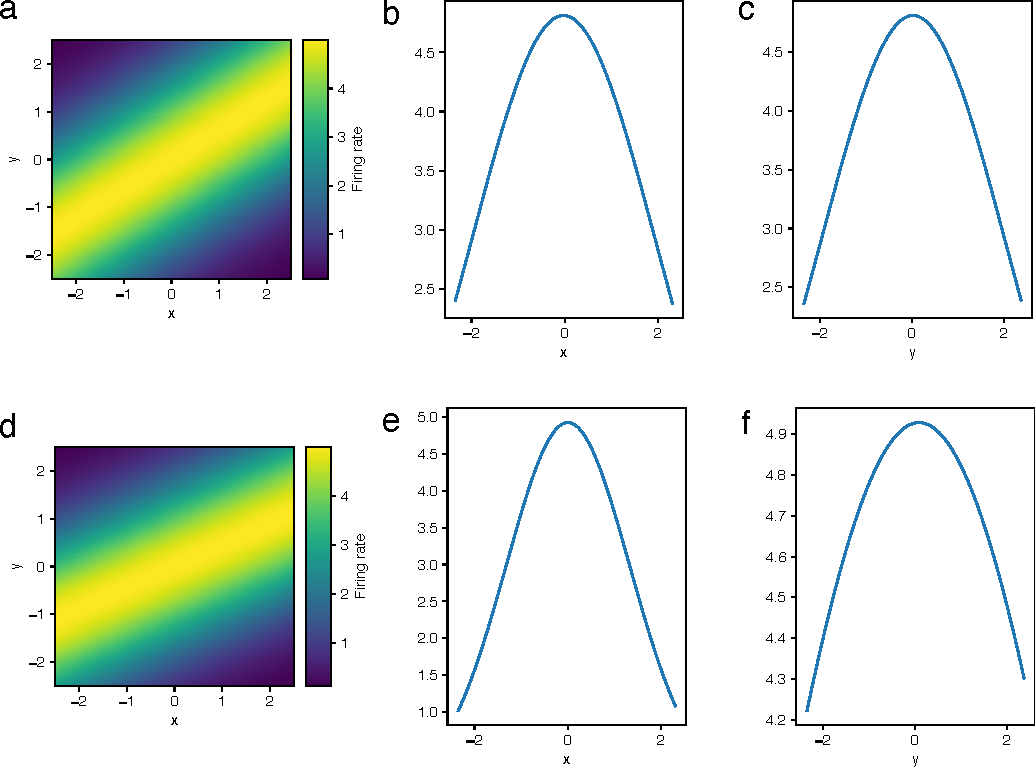
\includegraphics[width=0.8\textwidth]{Figures/fig2_glm.pdf}
    \caption{\textbf{The joint tuning curve may not be captured by the generalized linear model (GLM).} (a) The ground truth joint tuning curve for a hypothetical neurons. This neuron exhibit entangled joint tuning to variable $x$ and $y$. The marginal tuning for $x$ and $y$ are both flat.(b,c) If applying a GLM framework to analyze the simulated responses sampled from this neuron, the extracted marginal tuning using GLM would both be non-flat, thus is misleading. (d-f) Similar to (a-c), but for a different hypothetical model neuron.}
    \label{fig:glm}
\end{figure}

\section{Results}

\subsection{Marginal tuning curves are insufficient to capture the joint tuning}

When only one stimulus variable (denoted as $x$, such as the head direction of the animal) is considered, the tuning property of a given neuron can be described by its tuning curve $f(x)$. A tuning curve quantifies how the firing rate of a neuron varies as the stimulus variables changes.
Suppose that another stimulus variable $y$ is also of interest (e.g., the movement direction of the animal),
% the tuning curve $g(y)$ can also be computed separately for $y$. Suppose that 
and that our goal is to understand whether this neuron is selective to both $x$ and $y$. The standard approach would be to examine the marginal tuning curves $f(x)$ and $g(y)$ separately to see if one or both exhibit strong selectivity. Suppose that we find that $f(x)$ is a narrow Gaussian function, and $g(y)$ is completely flat, then it is tempting to claim that this neuron is selective to variable $x$, and it is not selectivity to (or it is invariant to) $y$. However, this analysis of the marginal tuning curves may lead to mis-interpretation of the joint tuning property to these two variables.  

Fig.~\ref{fig:glm} illustrates two such examples. The \textit{joint tuning map} $h(x,y)$ for the first example is plotted in Fig.~\ref{fig:glm}a. Examining the \textit{marginal tuning curves}, we see that $f(x)$ is tuned, while $g(y)$ is completely flat.
Although the marginal tuning curve for $y$ indicates a lack of selectivity, however, from the joint tuning map, the response of this neuron is clearly not invariant to $y$. What happens in this case is that the variability of neural response depends on $y$ through its interaction with $x$.
As another example (Fig.~\ref{fig:glm}d), the marginal tuning curves $f(x)$ and $g(y)$ are both flat. However, it would be unreasonable to claim that this neuron is invariant to $x$ and $y$ because its response clearly contains information about $(x,y)$. In fact, knowing the firing rate of the neuron would be informative for determining $(x, y)$. 
Importantly, the tuning of the two stimulus variables is highly entangled that can not be revealed by the marginal tuning curves. 

%There are certainly cases where one can interpret the joint tuning properties of the neurons directly based on the marginal tuning curves. One such scenario is that case that the 

% Fig XX illustrates one such example. In this case, this neurons is selective to variable $x$ and completely invariant to variable $y$. 
%Under the further assumption that $g(y)$ is flat and $f(x)$ is not flat, one can conclude that this neuron is selective to $x$ and invariant to $y$.

In the special case that the joint tuning map can be factorized into the product of marginal tuning curves, i.e., $h(x,y)=f(x)g(y)$, marginal tuning is sufficient to interpret joint tuning. There is indeed some evidence suggesting that for certain neurons and certain stimulus variables, there may be a multiplicative relationship between the joint tuning map and marginal tuning curves of individual behavioral variables~\cite{Hardcastle2017multiplexed}. 
Generalized linear model (GLM) framework that is often used in neural data analysis makes this important assumption~\cite{Pillow2008spatio}. Because in most applications of GLM, an exponential link function is assumed-- linearly adding responses in log of firing rates is equivalent to multiplying tuning curves.  However, in general, this multiplicative assumption should be carefully examined. When this assumption is violated, applying GLM to fit the data would lead to misleading results regarding the selectivity to the stimulus variables (see Fig.~\ref{fig:glm}). %[\textcolor{red}{We can consider dropping this paragraph if the GLM results do not help.}]
 
\begin{figure}[h!]
    \centering
    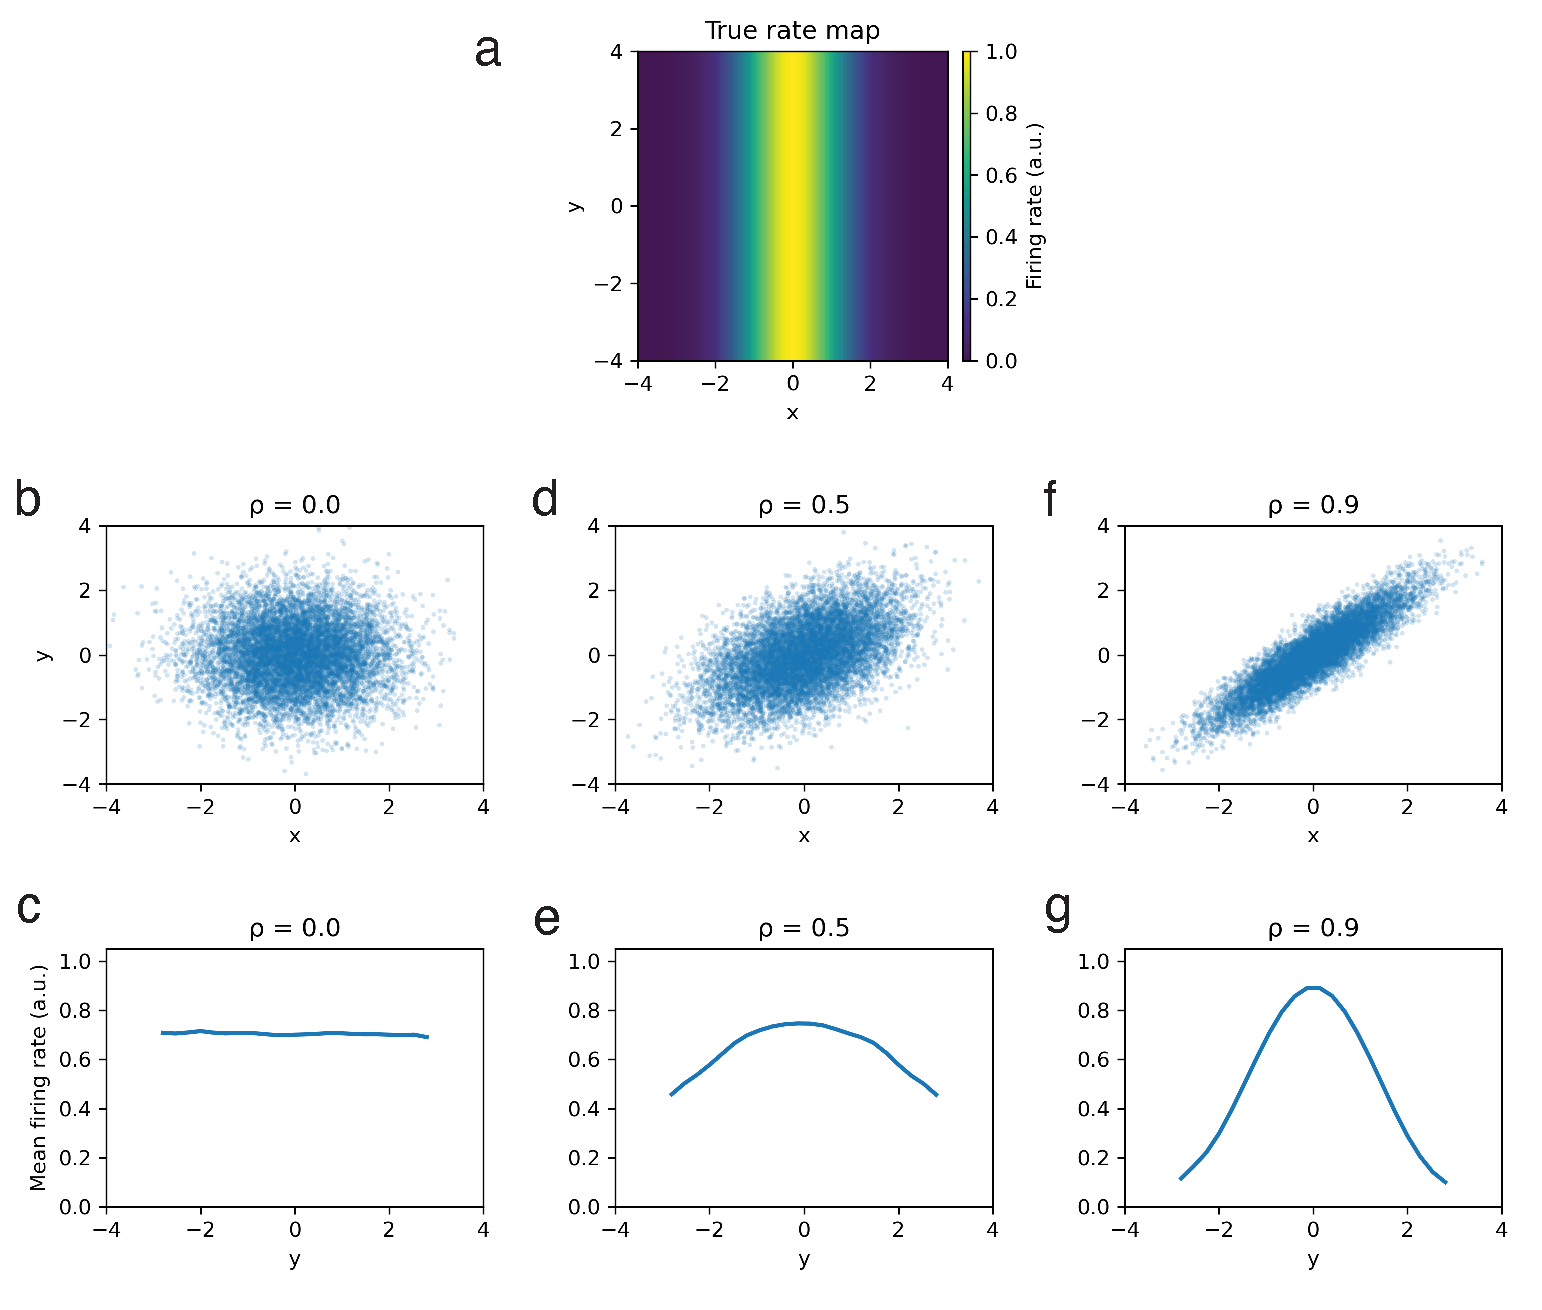
\includegraphics[width=0.8\textwidth]{Figures/CNN_fig1.pdf}
    \caption{\textbf{The joint tuning curve of a neuron cannot be adequately described by the marginal tuning.} (a) The joint tuning curves of a hypothetical neuron for variable $x$ and $y$. This neuron is selective to $x$, but is invariant to $y$. (b,c) When the samples of $x$ and $y$ are uncorrelated, empirically computed marginal tuning for $y$ accurately recover the ground truth tuning. (d,e) When the samples of $x$ and $y$ are correlated, empirically computed marginal tuning for $y$ would show selectivity. (f,g) Similar to (d,e), but for a case that $x$ and $y$ are even more correlated.  }
    \label{fig:fig1}
\end{figure}



%If a neuron is selective to multiple stimulus variables, this is often referred to as conjunctive tuning. More recently, ``mixed selectivity" is also used to describe the selectivity to multiple stimulus variables. If the multiplicative relationship between marginal and joint tuning holds, we will refer to it as linear mixing (because it is consistent with a GLM framework). Otherwise, we will refer to it as nonlinear mixing. 


The interpretation of marginal tuning curves may be further complicated by correlated sampling of the stimuli. Consider the case of studying the neural tuning of two correlated stimulus variables. Correlated stimulus variables are fairly common. In the study of spatial navigation, one notable example is the animal's head direction and movement direction~\cite{Raudies2015head}. Another example is the time and distance traveled when the animal is running on a linear track. Suppose that a neuron is selective to one variable $x$, while being completely invariant to the other variable $y$ (see Fig.~\ref{fig:fig1} for an example).  Due to the correlation in the stimulus sampling, the marginal tuning for $y$ would still suggest substantial selectivity (see Methods for more theoretical results).  In this case, if we only rely on the marginal tuning curves to interpret the tuning properties, we would incorrectly conclude that the neuron is tuned to $x$, although its response is completely invariant to $x$. Direct analysis of the joint tuning would be needed in these cases.

%It is evident that the marginal tuning curve on head direction is also narrowly tuned. This is due to biased sampling in the stimulus space. 




%An alternative approach would be to fit a GLM model to the neural response directly. To assess whether GLM can correctly identify the regime of correlated sampling, we generate simulated neural response from the model above, and fit GLM to the model responses.  Fig.~\ref{fig:glm} show a couple of examples under this setting. We find that GLM may falsely report strong selectivity to a given stimulus variable despite of the absence of such selectivity in the marginal tuning. These results suggest that the popular GLM approach also failed in accurately characterizing the joint tuning properties. 

%\textcolor{red}{Testing if GLM can recover the invariance for the second dimension in cases the neuron is only selective the first dimension and the stimulus sampling is biased.  }

%\textcolor{red}{Add a figure on GLM to show the model recovery with correlated sampling, and when the two dimensions are not multiplicative.}






\subsection{A method for analyzing the invariance and selectivity of neurons}

The above results show that, when analyzing the selectivity and invariance of the neural response properties, it is crucial to examine the joint tuning properties beyond marginal tuning curves. How should we study the contribution of an individual stimulus variable to the neuron's activity?
%Relying on marginal tuning curves alone may lead to misinterpretation of the tuning properties. 
%How should we quantify the joint tuning properties of an individual neuron? %To our knowledge, no systematic tools have been developed in the field. 
Practically, one simple procedure to get a sense of whether the neural response is invariant to a stimulus variable $x$ is to vary $x$ and examine the tuning for the remaining variables-- if only two variables are considered, this amount to examine the tuning curve of $y$ \textit{conditioned on} different values of $x$. 
If the tuning curve for $y$ is invariant when changing $x$, one may conclude that the response of this neuron is invariant to $x$. Otherwise, the response of this neuron depends on variable $x$. In other words, variable $x$ contributes to the response variability of this neuron. 
%It is important to note that such dependence may take different forms depending on the problems and neurons studied. One simple form of dependence is a gain change. That is, if varying $x$ leads to a multiplicative change of the tuning curves for $y$, the joint tuning for $x,y$ can be factorized into a product of the marginal tuning for $x$ and $y$.


\begin{figure}[h!]
    \centering
    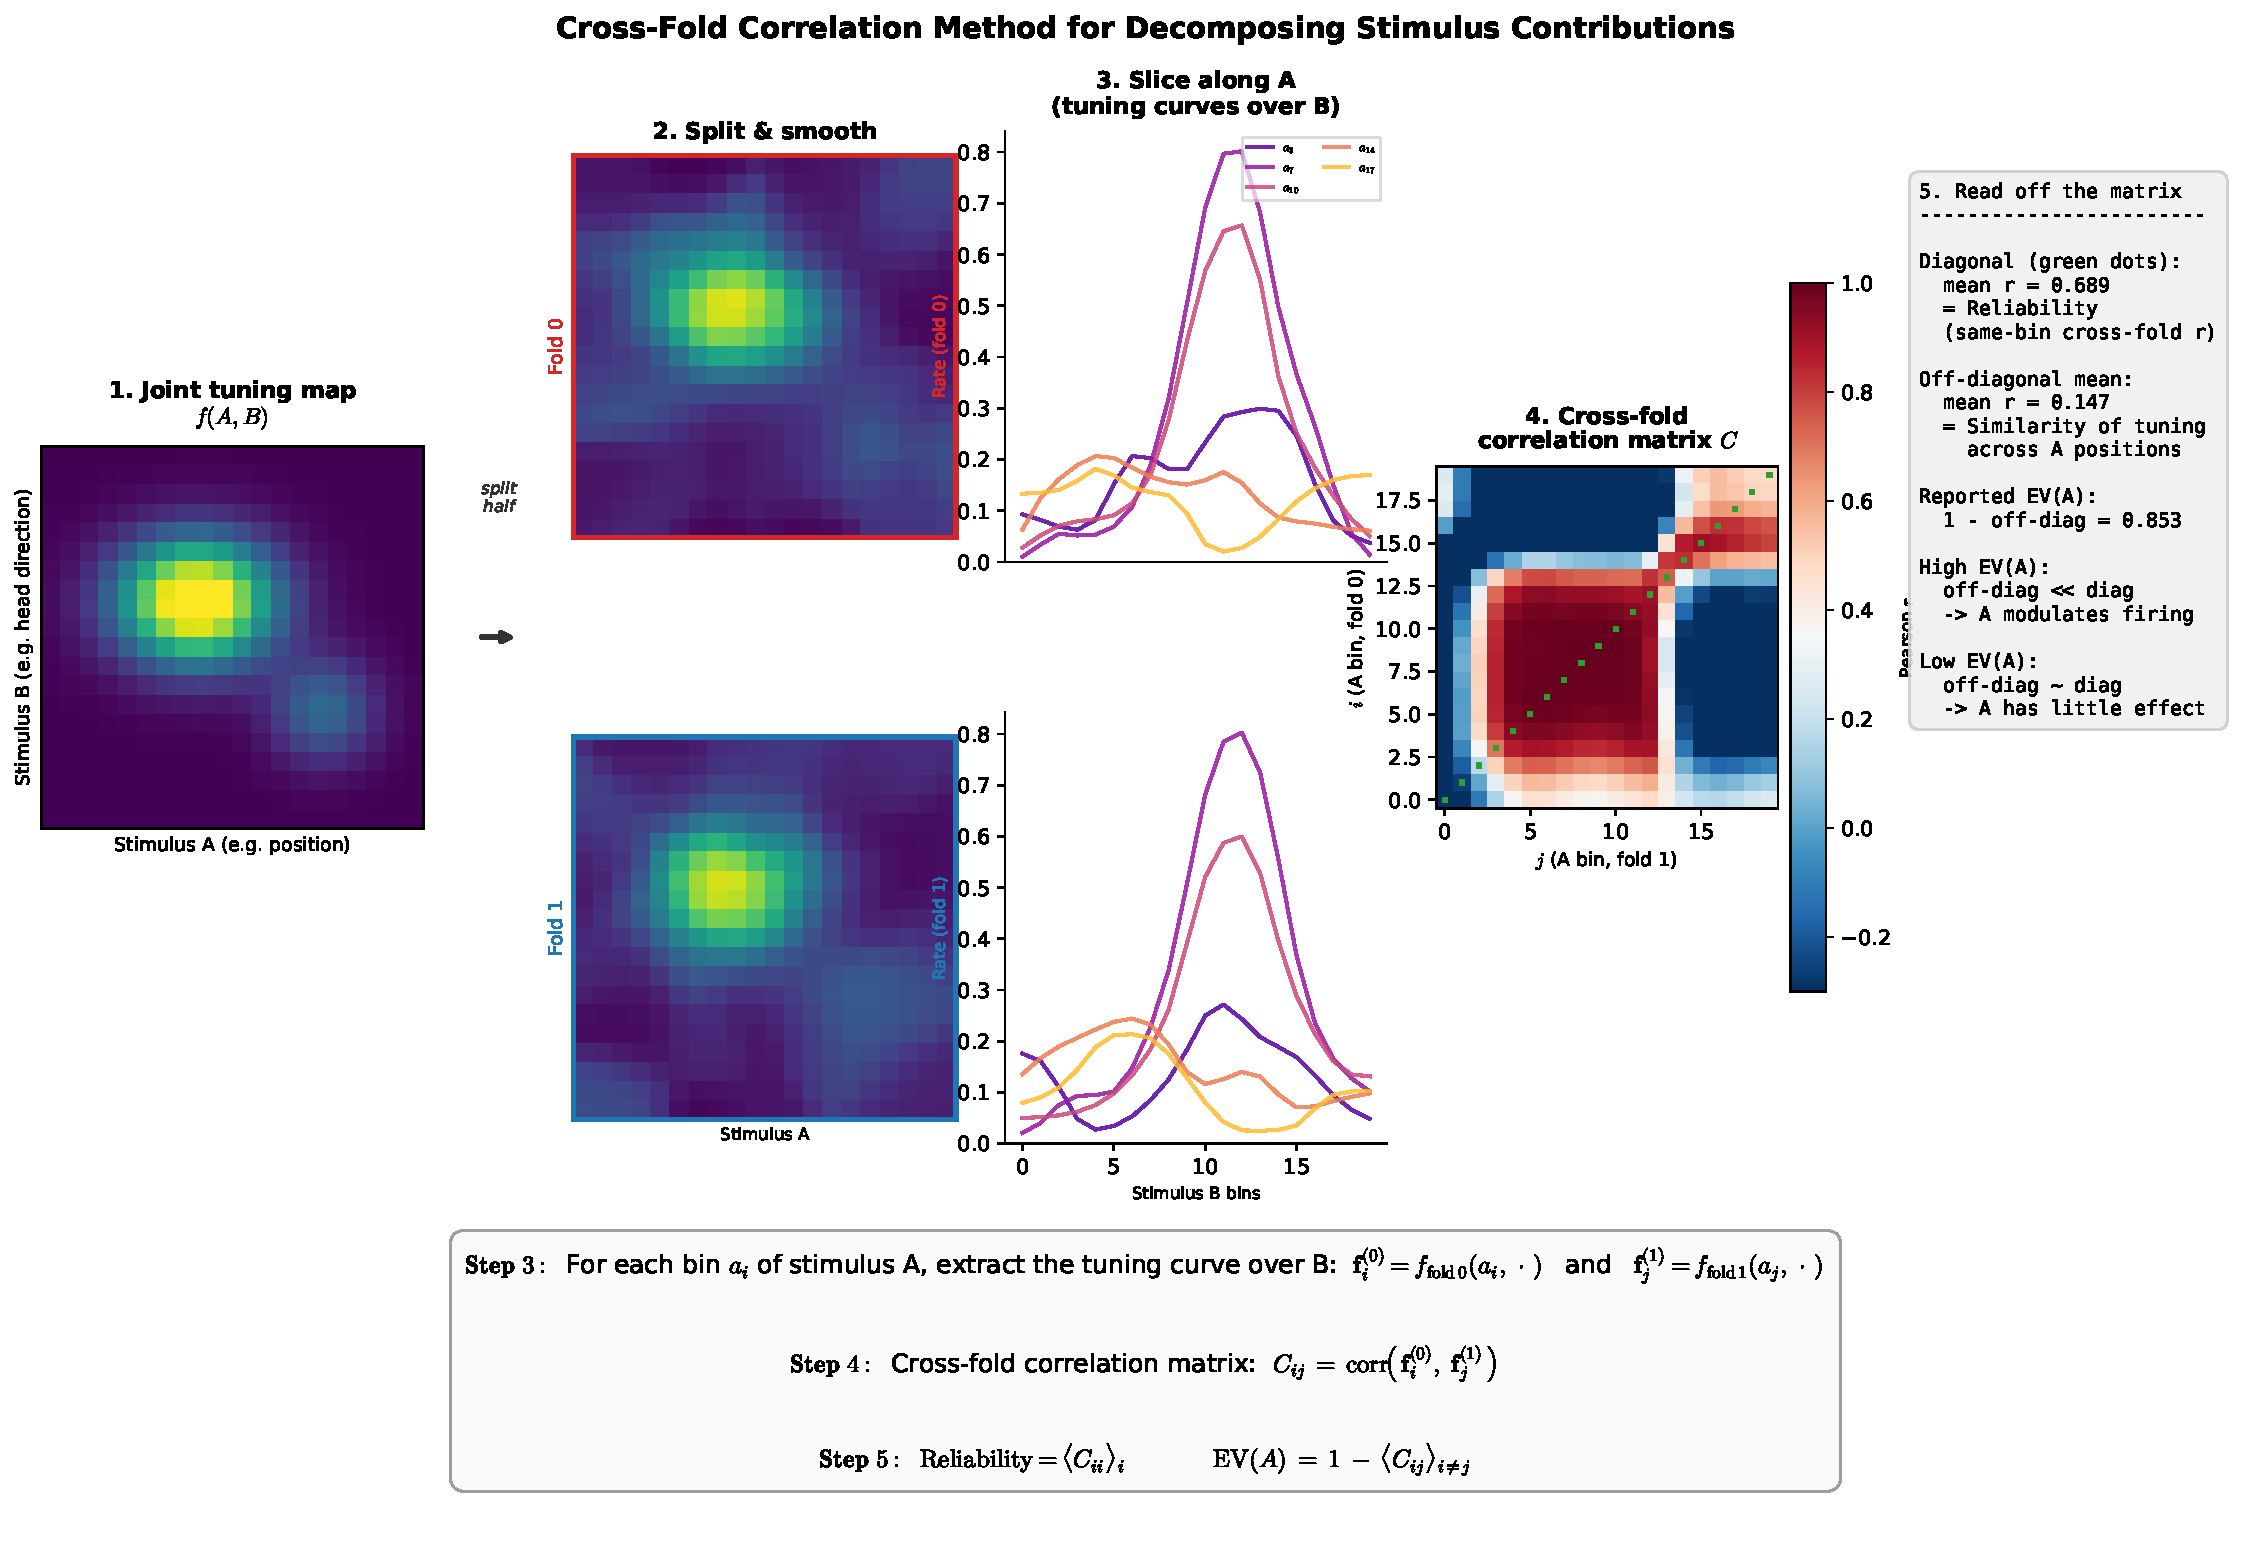
\includegraphics[width=0.72\textwidth]{figs/method_schematic.pdf}\\[4pt]
    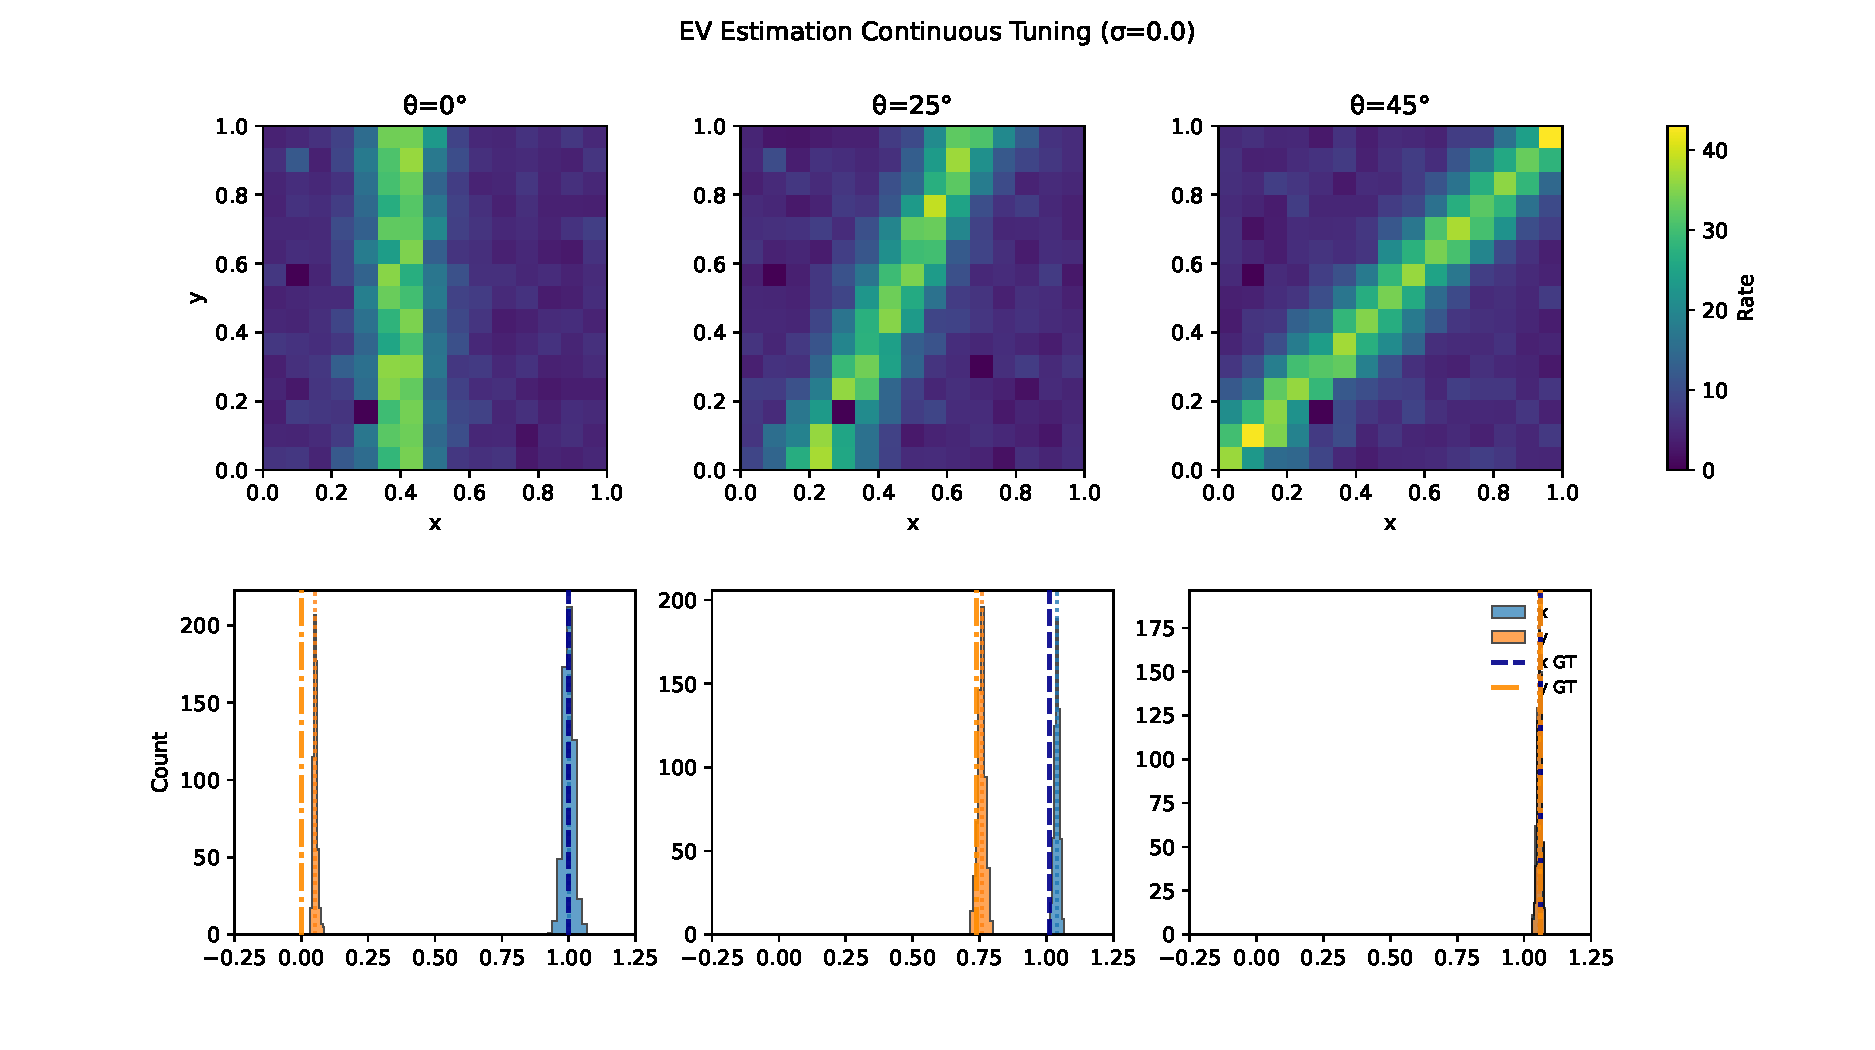
\includegraphics[width=0.68\textwidth]{figs/smoothed_binning_fig_corr.pdf}
    \caption{\textbf{The contribution of each stimulus variable can be quantified with the cross-fold correlation method.}
    (Top) Schematic of the estimation procedure for the contribution of stimulus $A$. The data are split into two halves and a joint tuning map is estimated from each fold. Each map is sliced at every value of $A$ to obtain tuning curves over the other variable $B$; the tuning curve at $a_i$ in fold~0 is correlated with the tuning curve at $a_j$ in fold~1 to form the cross-fold correlation matrix $C_{ij}$ (Eq.~\ref{eq:1}). The mean diagonal is the split-half reliability of the maps; the contribution of $A$ is $\mathrm{EV}(A)=1-\langle C_{ij}\rangle_{i\neq j}$ (Eq.~\ref{eq:2}). For mathematical details, see Methods.
    (Bottom) Validation on simulated Poisson responses to a Gaussian ridge rotated by $\theta=0\degree$, $25\degree$ and $45\degree$ on a $15\times 15$ grid (top row: estimated joint tuning maps from one simulation). Histograms show $\mathrm{EV}(x)$ (blue) and $\mathrm{EV}(y)$ (orange) over 600 random split-half partitions; dashed lines mark the ground truth computed from the noiseless tuning map. At $\theta=0\degree$ the neuron depends on $x$ only and the estimator recovers $\mathrm{EV}(x)\approx 1$ and $\mathrm{EV}(y)\approx 0$; the small positive bias on the untuned axis ($\approx 0.05$) is the finite-sampling floor $1-\langle C_{ii}\rangle$ of the split-half estimate. At $\theta=45\degree$ both variables contribute equally. Note that $\mathrm{EV}$ can marginally exceed 1 when tuning curves at distant positions are anticorrelated (Methods). The size of this floor depends only on how densely the joint map is sampled (Supplementary Fig.~\ref{fig:si_floor}); a discrete look-up-table version of the tuning function gives identical results.
    }
    \label{fig:estimation}
\end{figure}




To understand the contribution of individual variables taking into account their nonlinear interactions, we develop a simple analysis approach using the joint tuning map, based on the intuition described above. As an example, to quantify the contribution of variable $x$, we ask how much the neuron's tuning over $y$ changes across different values of $x$. Specifically, we slice the joint tuning map at each value of $x$ to obtain tuning curves over $y$, and then compute the pairwise Pearson correlation between tuning curves at different $x$ positions. If these tuning curves are all similar, $x$ contributes little; if they differ substantially, $x$ is an important driver of the response. The contribution of $y$ can be computed symmetrically by slicing along the other axis. %Unlike analysis of variance (i.e., ANOVA) for linear additive models, summing up the contribution of $y$ and $x$ may not be equal to the total variance of the data.

Practically, one complication in estimating the contribution of individual variables is measurement noise. Consider the case mentioned above in which the neural response is selective to $x$ while being completely invariant to $y$. Due to measurement noise, tuning curves estimated from finite data will exhibit spurious differences across positions, which would lead to overestimation of a variable's contribution. To address this problem, we compute the correlations across two independent halves of the data: each tuning curve in one fold is correlated with tuning curves from the other fold. Because the noise in the two folds is independent, it cannot inflate the cross-fold correlations, yielding an estimate that is robust to measurement noise (see Methods).
%A schematic of our proposed analysis procedure is shown in Fig.~\ref{fig:estimation}a. 
%Our mathematical analysis shows that the proposed estimator (details see the Method Section) is unbiased under the assumption that measurement noise is independent across the two halves. 
We perform systematic simulations to validate and benchmark our noise-corrected estimator based on split-half analysis. We find that the estimation procedure can well recover the relative contribution of each variable (for an example, see Fig.~\ref{fig:estimation}d,e). %However, there are also cases that the estimation error is more substantial given limited amount of data .

%As a complementary approach to the non-parametric approach described above, we also considered a parametric approach by constructing models based on mixture of product of Gaussian functions. In the case of having only one mixture component, the model reduces to one that assume (i) the marginal tuning of the two variables are both Gaussian; (ii) a multiplicative interaction between the tuning to the two variables. By incorporating multiple components, the model is more flexible than the standard GLM and allows more complex patterns of mixing of the tuning properties. In applications, one interesting question is whether models with multiple mixture components would outperform the standard one component model. Because each mixture component is parameterized by Gaussian function with only a few parameters, this mixture model remain feasible in fitting to limited amount of experimental data.

%\subsection{Place cells are selective to location and invariant to head direction}

\subsection{Model units in deep network models based on vision exhibit entangled pattern of spatial tuning}

Despite that many previous studies suggest that path integration is important for the formation of cognitive maps in the brain~\cite{Mcnaughton2006,Burak2009,Cueva2018}, recent studies reported that place cell-like response in deep neural networks trained or pretrained to perform vision tasks alone~\cite{Luo2024,Gornet2024automated}. In \cite{Gornet2024automated}, it was reported that training a virtual navigation agent to predict the next image frame led to the formation of cognitive maps. In particular, neurons in certain hidden layers exhibit selectivity to the agent's location, similar to place cells. Meanwhile, Luo et al analyzed the response of individual units in ResNet (pretrained on image classification tasks, or untrained) in a spatial environment~\cite{Luo2024}, and reported that a large fraction of model units throughout the network layers exhibit spatial selectivity (to location or head direction).  Importantly, these studies \cite{Luo2024,Gornet2024automated} only examined the marginal tuning to these spatial variables (e.g., location or head direction separately) without examining their joint tuning properties. %Thus, it remains unclear whether the joint tuning for place and HD would be similar to that of hippocampus place cells. 
As we showed above, marginal tuning alone may miss important information of the neural representation, thus here we
seek to examine the joint tuning of units in the types of deep network models studied in \cite{Luo2024,Gornet2024automated} to better understand their response properties. Later we will test these predictions using data from the spatial navigation systems in the rodent brain. 
%We hypothesize that while the model neurons may exhibit place fields when examining the marginal tuning for location, the model neurons may not exhibit invariance to HD as in hippocampal place cells. 


{\bf Model units in networks trained on predictive coding exhibit entangled spatial tuning}
Inspired by prior work on predictive coding~\cite{Srinivasan1982predictive,Rao1999predictive}, Gornet et al \cite{Gornet2024automated} trained a virtual navigation agent, implemented as a deep neural network, to predict the next image frame in a temporal sequence of images as the agent moves in space (Fig.~\ref{fig:pred}a). They then analyzed the responses properties of model neurons in the intermediate layers, and found that these neurons show place-cell-like responses. 

We re-implemented the training setting using a Mine-Craft environment similar to \cite{Gornet2024automated}. After training the simulated agent to solve the next-frame image prediction task, we investigated the response properties of model units in different layers of the model.
%(see \textcolor{red}{SI Fig. XX for the performance of the agent in this prediction task}). 
As the head direction of the simulated agent are allowed to vary, we can obtain the response of individual model units corresponding to different combinations of 2-D locations and head direction.
%Note that in the basic version of the model reported in \cite{Gornet2024automated}, the head direction of the virtual agent is assumed to be fixed, which is not realistic. 
Examining the response properties of model units using established metrics in the place field literature~\cite{Tanni2022}, we find that a fraction of them in the intermediate layers can be classified as putative place cells (see Fig.~\ref{fig:pred}b), consistent with the original reports in~\cite{Gornet2024automated}. We next investigate the joint tuning of 2-D location and head direction. Strikingly, we find that model units generally exhibit complex and highly tangled tuning for location and head direction (see Fig.~\ref{fig:pred}c for example model units). When conditioned on different head directions, the tuning curves for locations, visualized as 2-D heatmaps, clearly change (Fig.~\ref{fig:pred}c). Thus, the location selectivity of model units lacks invariant to the head direction. 


Quantification of variance explained by location and head direction for individual units based on the methods developed above shows that the responses of most individual model units were roughly equally explained by the head direction and location (Fig.~\ref{fig:pred}, bottom row; pre-prediction layer: median $\mathrm{EV}_{xy}=0.93$, median $\mathrm{EV}_{hd}=0.92$, $n=8{,}000$ units, of which $54\%$ were location-dominant). Furthermore, we selectively analyzed the model units identified as putative place cells and found similar results, except that these unit show a slightly higher percentage of variance explained than other units.
%This entangled tuning properties is clearly different from place cells in rodents (and is also different from the head direction cells). 
We additionally analyzed other layers beyond the intermediate attention layers examined in~\cite{Gornet2024automated} and found consistent results across different layers of the network (see Supplementary Fig.~\ref{fig:si_pred_ev}).
%(\textcolor{red}{Add some SI figures on this}). 

%It is also consistent in different versions of the models we trained, thus is insensitive to the idiosyncratic details of the networks.

%We perform similar analysis on a different network that were trained on different task objectives. In ref XX, they trained neural network to predict the next frame of visual inputs for a navigation agent. They found place-cell-like representation in the later layer of the network. In their basic model, the head direction of the virtual agent is assumed to be fixed, which is not realistic. It is possible to modify their model framework to make head direction variable. We trained this augmented version of the model and examine the model units throughout the network. 


\begin{figure}[h!]
    \centering
    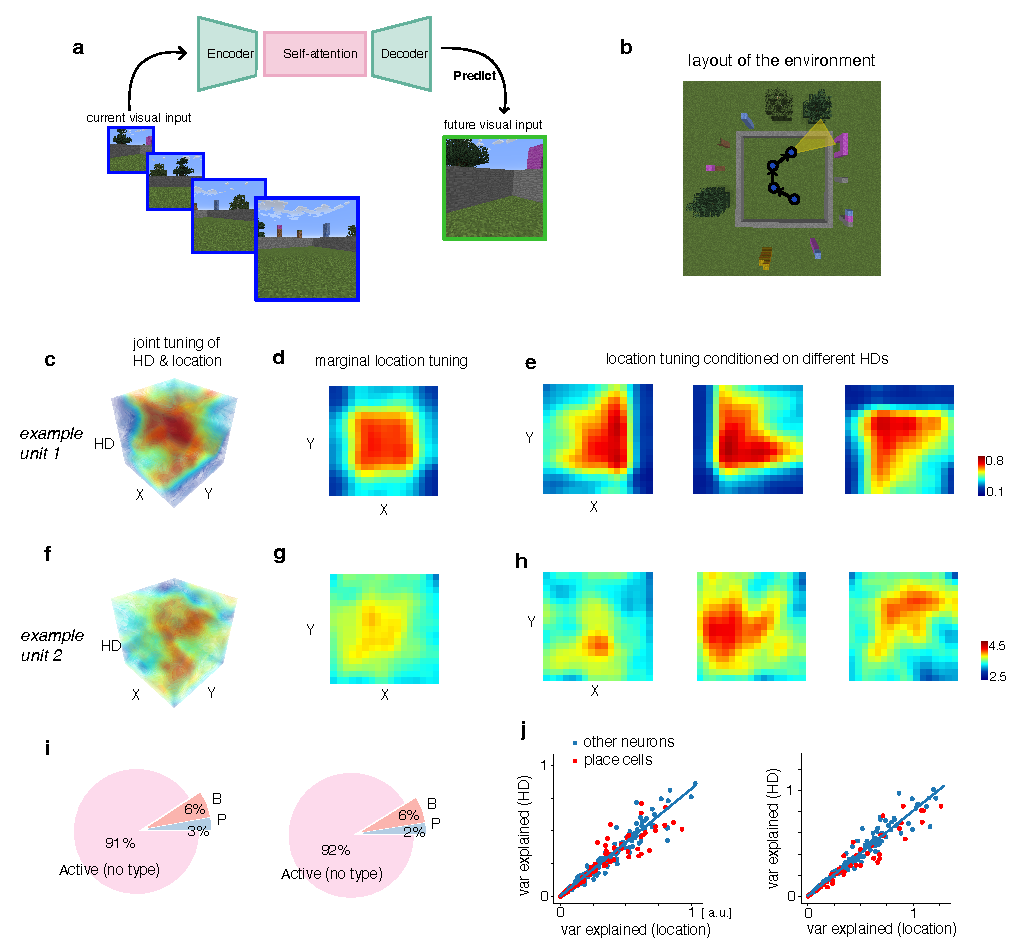
\includegraphics[width=0.8\textwidth]{Figures/Fig_pred coder_ver2.pdf}\\[2pt]
    % TODO(author): panel (j) inside the composite above still shows the superseded variance-based estimator; regenerate the composite with the two panels below (pre_pred, post_pred) in its place.
    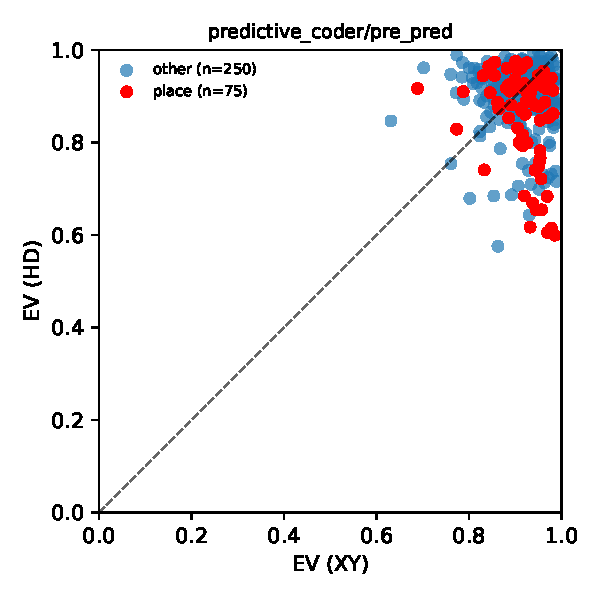
\includegraphics[width=0.27\textwidth]{figs/predictive_coder_pre_pred_ev_pitch.pdf}\hspace{0.04\textwidth}
    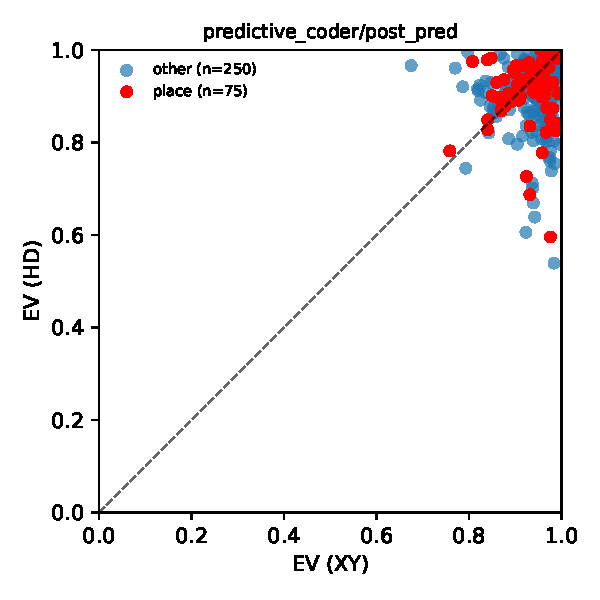
\includegraphics[width=0.27\textwidth]{figs/predictive_coder_post_pred_ev_pitch.pdf}
    \caption{\textbf{Model neurons in deep networks trained to predict the next image frame exhibit highly entangled tuning properties for location and head direction.} (a) A schematic of the modeling framework used in \cite{Gornet2024automated}. Adapted from \cite{von2024cognitive}. (b) Layout of the virtual environment. (c--h) Two example model units classified as place cells: joint tuning of location and HD (c,f), marginal location tuning (d,g), and location tuning conditioned on different head directions (e,h). While the marginal 2-D map exhibits a place field, the location tuning clearly changes with HD. (i) Pie charts showing the fraction of model units classified as place (P) or border (B) cells in two layers of the model. (j) Superseded panel (earlier variance-based estimator; see TODO in source). Bottom row: variance explained by location ($\mathrm{EV}_{xy}$) versus head direction ($\mathrm{EV}_{hd}$) with the cross-fold correlation estimator (Eq.~\ref{eq:2}) for every unit in the pre-prediction (left) and post-prediction (right) latent layers; red points are units classified as place cells; the dashed line marks $\mathrm{EV}_{xy}=\mathrm{EV}_{hd}$. }
    %\textcolor{red}{Add a figure showing the environment we constructed. Also, which equation did we use to quantify the contribution? I think we should use the noise-free version.} }
    \label{fig:pred}
\end{figure}

%We first classify tentative model place cells using commonly used procedure in analyzing place cells. We then analyze the invariance of these neurons to HD, and find...






{\bf Pre-trained convolutional neural networks (CNNs) also exhibit an entangled spatial tuning}  We next investigate another recently proposed model based on deep neural networks pre-trained to perform image classification tasks. Convolutional neural network models (CNNs) have become a popular modeling framework in understanding how the brain process visual information~\cite{Yamins2014,Khaligh2014,Yamins2016}. Luo et al~\cite{Luo2024} proposed to use CNNs to study the navigation system in the brain. Specifically, they modeled the visual inputs of an virtual agent navigating in a 2-D open area that was similar to the typical environments for rodent neurophysiology experiments. Importantly, these CNNs are pretrained on visual tasks and only receive visual inputs, with no inputs on the agent's velocity. %Naively one would expect that the model units based on pure visual inputs should not lead to spatial selectivity. 
%Somewhat surprisingly, t
~\cite{Luo2024} reported that many model units in the network throughout the layers exhibit place cell-like responses, as well as head direction tuning.


\begin{figure}[h!]
    \centering
    \subfigure[\texttt{layer1}]{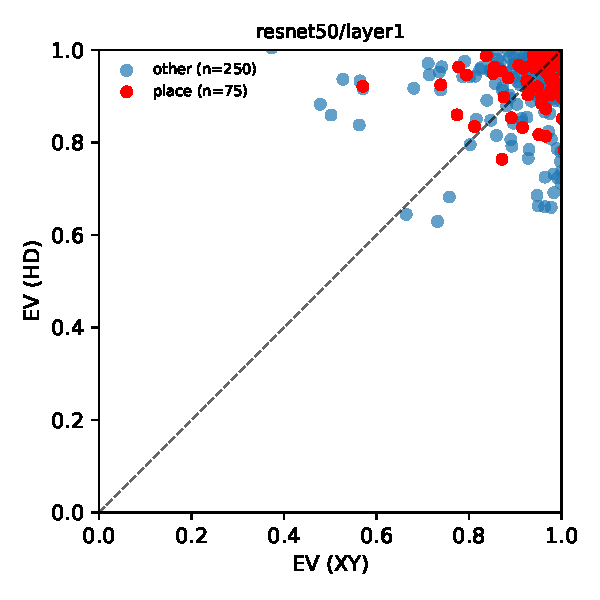
\includegraphics[width=0.24\textwidth]{figs/resnet50_layer1_ev_pitch.pdf}}
    \subfigure[\texttt{layer3}]{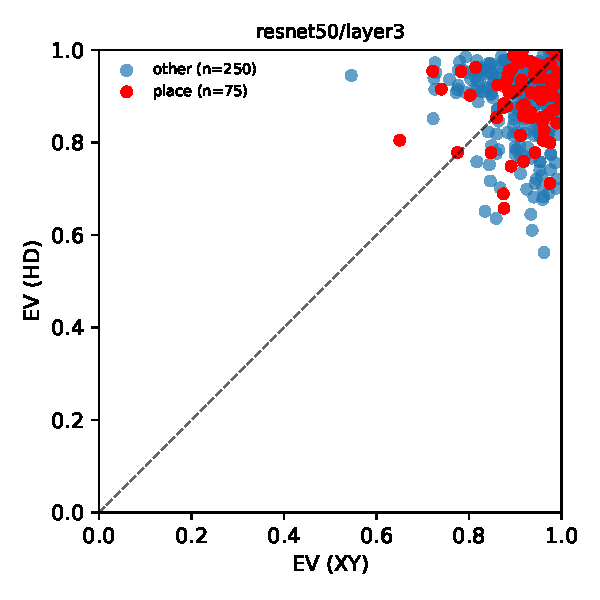
\includegraphics[width=0.24\textwidth]{figs/resnet50_layer3_ev_pitch.pdf}}
    \subfigure[\texttt{layer4}]{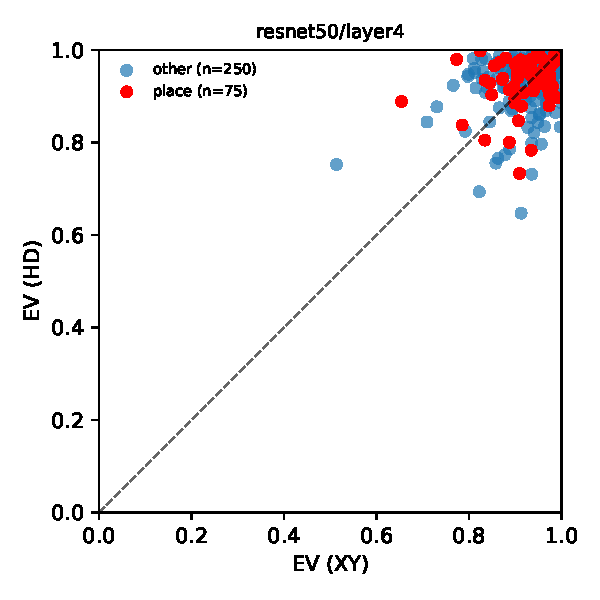
\includegraphics[width=0.24\textwidth]{figs/resnet50_layer4_ev_pitch.pdf}}
    \subfigure[\texttt{avgpool}]{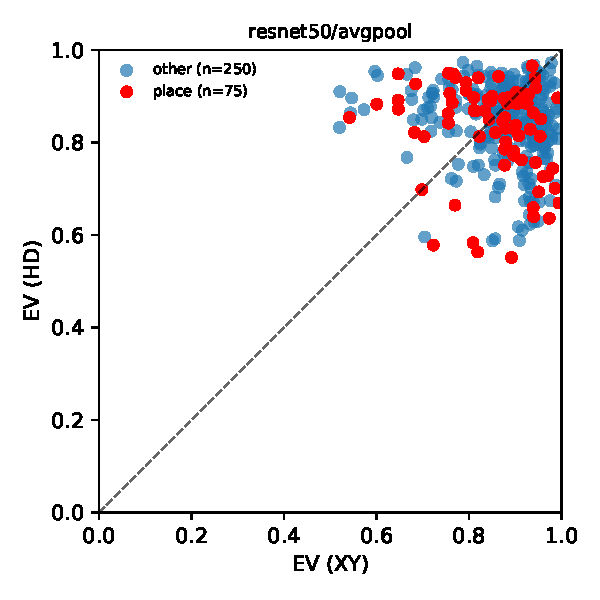
\includegraphics[width=0.24\textwidth]{figs/resnet50_avgpool_ev_pitch.pdf}}
    \caption{\textbf{Model neurons in CNNs trained on image recognition tasks exhibit highly entangled tuning properties for location and head direction.} (a-d) Variance explained by location ($\mathrm{EV}_{xy}$) versus head direction ($\mathrm{EV}_{hd}$) for individual model units in four layers of an ImageNet-pretrained ResNet-50 (\texttt{layer1}, \texttt{layer3}, \texttt{layer4}, and \texttt{avgpool}), estimated with the cross-fold correlation method (Eq.~\ref{eq:2}). Red points are units classified as putative place cells; the dashed line marks $\mathrm{EV}_{xy}=\mathrm{EV}_{hd}$. In every layer the population lies on the diagonal (median $\mathrm{EV}_{xy}$ and $\mathrm{EV}_{hd}$ both $\approx 0.9$): the two variables contribute equally to the response variability, unlike the place cells and head direction cells in the brain. Results for a VGG-16 layer and an untrained ResNet-50 are shown in Supplementary Fig.~\ref{fig:si_cnn_ev}.}
    \label{fig:CNN}
\end{figure}


%\textcolor{red}{Add some example neurons tuning curves, and the quantification using our method}



We sought to replicate their main results using the same Mine-Craft environment developed above, which is similar (although not identical) to the environment used in \cite{Luo2024}.
%except that we did not find a large fraction of model units that are selective to head direction when analyzing the marginal tuning curves of individual neurons for HD. 
We took a CNN (ResNet50) pretrained to perform image classification tasks, and collected the response of this CNN in the Mine-Craft virtual environment.  We first analyzed the marginal tuning for location and HD in the CNN. Indeed, consistent with the results in \cite{Luo2024}, we found that a fraction of model units exhibit putative place fields in 2-D space. Notably, \cite{Luo2024} also reported that many model units exhibit strong head direction tuning and a subset of neurons exhibit conjunctive place and HD tuning. Our own analysis of marginal tuning suggests that few model units are tuned to HD, and consequentially, few units are tuned to both HD and location. Examining the code released accompanied by~\cite{Luo2024}, we found that their criteria could not properly capture the selectivity to head direction. When we tried their method for classifying head direction cells, we also found that many model units in our network would be classified as head direction cells. These results suggest that the difference in the prevalence of units with head direction tuning between ours and theirs are primarily due to the issue with the analysis in \cite{Luo2024}, not the difference in the virtual environments used.

%At face value, this seems to suggest that the model units exhibit properties similar to place cells in rodents. Again, as noted earlier, according to our results earlier it is necessary to examine the joint tuning of place and HD to better compare the two.

To investigate the joint tuning to location and space, we again examine the 3-D place and HD maps for the model units that are classified as tentative place cells. We find that the firing fields are highly scattered in the 3-D space (see Supplementary Fig.~\ref{fig:si_scattered_maps}), and typically
%The location of the putative place fields varies depending on the HD.  
the model unit only generated high activity with particular combinations of place and HD. This basic observation is similar to what we discovered in the network trained on prediction task. We further quantify the variance of individual neurons explained by location and head direction in different layers of the network. Across all layers, location and head direction explain about equal amount of variance for individual model units (see Fig.~\ref{fig:CNN} for results from four example layers from a CNN; all analyzed layers are shown in Supplementary Fig.~\ref{fig:si_cnn_ev}), similar to Predictive Coding Network. 
%Again, their response properties are clearly different from those of the place cells and head direction cells from the brain. 


Together, our results replicated some of the key findings reported in recent studies that investigate spatial tuning properties in deep neural networks trained on purely visual tasks. Indeed, when analyzing the marginal tuning for 2-D location, a fraction of model neurons have putative place fields. Importantly, our analysis of joint tuning reveals a striking new insight about the properties of spatial selectivity in these deep network models. That is, the tuning for spatial location and head direction are strongly entangled. For most model units, location and head direction explain about equal amount of variance in the response. Therefore, in these models, there are not distinct populations that are encoded head direction and spatial location separately. 


%We also visualize the joint tuning of HD and the first dimension of space, and the joint tuning of HD and the second dimension of space. The results again show that the response of models units are not invariant to HD. 

%We compute the location map for four different HDs, and then evaluate the correlation between these maps. We find that the correlation is ...This is much smaller than what we found in hippocampus place cells.

%We further quantify the variance of the firing rate map explained by HD and location and found that the two explain about similar amount of variability. This suggests that the tuning for HD and location are highly entangled. We compared these results to what we obtained from the rat hippocampus (see Fig. XX). 

%We reason that this highly mixed code may due to that (i) the model units are encoding visual features, and (ii) the visual features in the environment are related to the HD and location in a complicated way. Only a particular combination of HD and location may result in the particular visual feature preferred by a model unit. To test this idea, we examine the model units in the first layer of the network for which their response properties can be easily interpreted using the receptive fields. In particular, we identify neurons with oriented receptive fields and examine their place and HD tuning. We find... We conclude that the model units were not encoding location per se, instead they form a high mixed code that represents particular combination of head direction and location. This code is qualitative and quantitative different from the place code in the rat hippocampus. 

%One should be able to decode HD from the model response.


%\textcolor{red}{Add some example neurons tuning curves, and the quantification using our method}



\FloatBarrier
\subsection{Distinct selectivity and invariance of place cells and head direction cells in rodent brain}

We next investigate the tuning properties of neurons recorded in rodent spatial navigation system and compare them to results from the deep network models above. We will analyze two datasets. The first is a place cell dataset recorded from the hippocampus when rats were navigating in 2-D environments~\cite{pfeiffer2015}. The second dataset contains head direction cells recorded from multiple brain regions~\cite{Duszkiewicz2024}. In addition to their selectivity to spatial variable based on which these cell types were defined, we are interested in whether they are invariant to other  variables, e.g., whether place cells are invariant to head direction. 
%To address these questions, we will use our proposed analysis framework to understand the joint tuning together with population decoding techniques. 

%neural responses in the hippocampus recorded when the rats were performing a navigation task in a two-dimensional open environment. This dataset were originally published in \cite{pfeiffer2015}. 


\textbf{Place cells in the rat hippocampus is invariant to head direction} As a first analysis on the place cell dataset (\cite{pfeiffer2015}), we calculated the 2-D spatial firing rate maps for individual neurons. Consistent with previous reports a large fraction of rat hippocampal neurons are selective to spatial location in the 2-D open environment, with clear circular-shaped place fields. 
%and they typically have one or two place fields.
Computing the marginal tuning curve for head direction, we find that most place cells do not exhibit strong head direction tuning, consistent with previous reports. 
%While it has been documented that most place cells were not tuned to head direction (also confirmed by our own analysis on marginal tuning of head direction),
However, at this point, it remains unclear whether these neurons exhibit strong invariance to head direction, recalling that our theoretical results above suggest that even when the tuning curve for a stimulus is flat, neural responses may still depend on the stimulus (Fig.~\ref{fig:glm}). To further investigate this question, we computed the joint tuning map for location and HD. For each neuron, this results in a 3-D heatmap (see Fig.~\ref{fig:PlaceCell}a,b for examples). Visual inspection suggests that the neural response is highly structured and is largely invariant to HD. When conditioned on the head directions, the locations of the place fields are stable. We did also observed that the peak firing rates of place fields varies modestly across different slices, suggesting that head direction multiplicatively modulates the place field response.

%However, due to limited data, some combinations of HD\&location have few or no data points. 

\begin{figure}[h!]
    \centering
    \subfigure[]{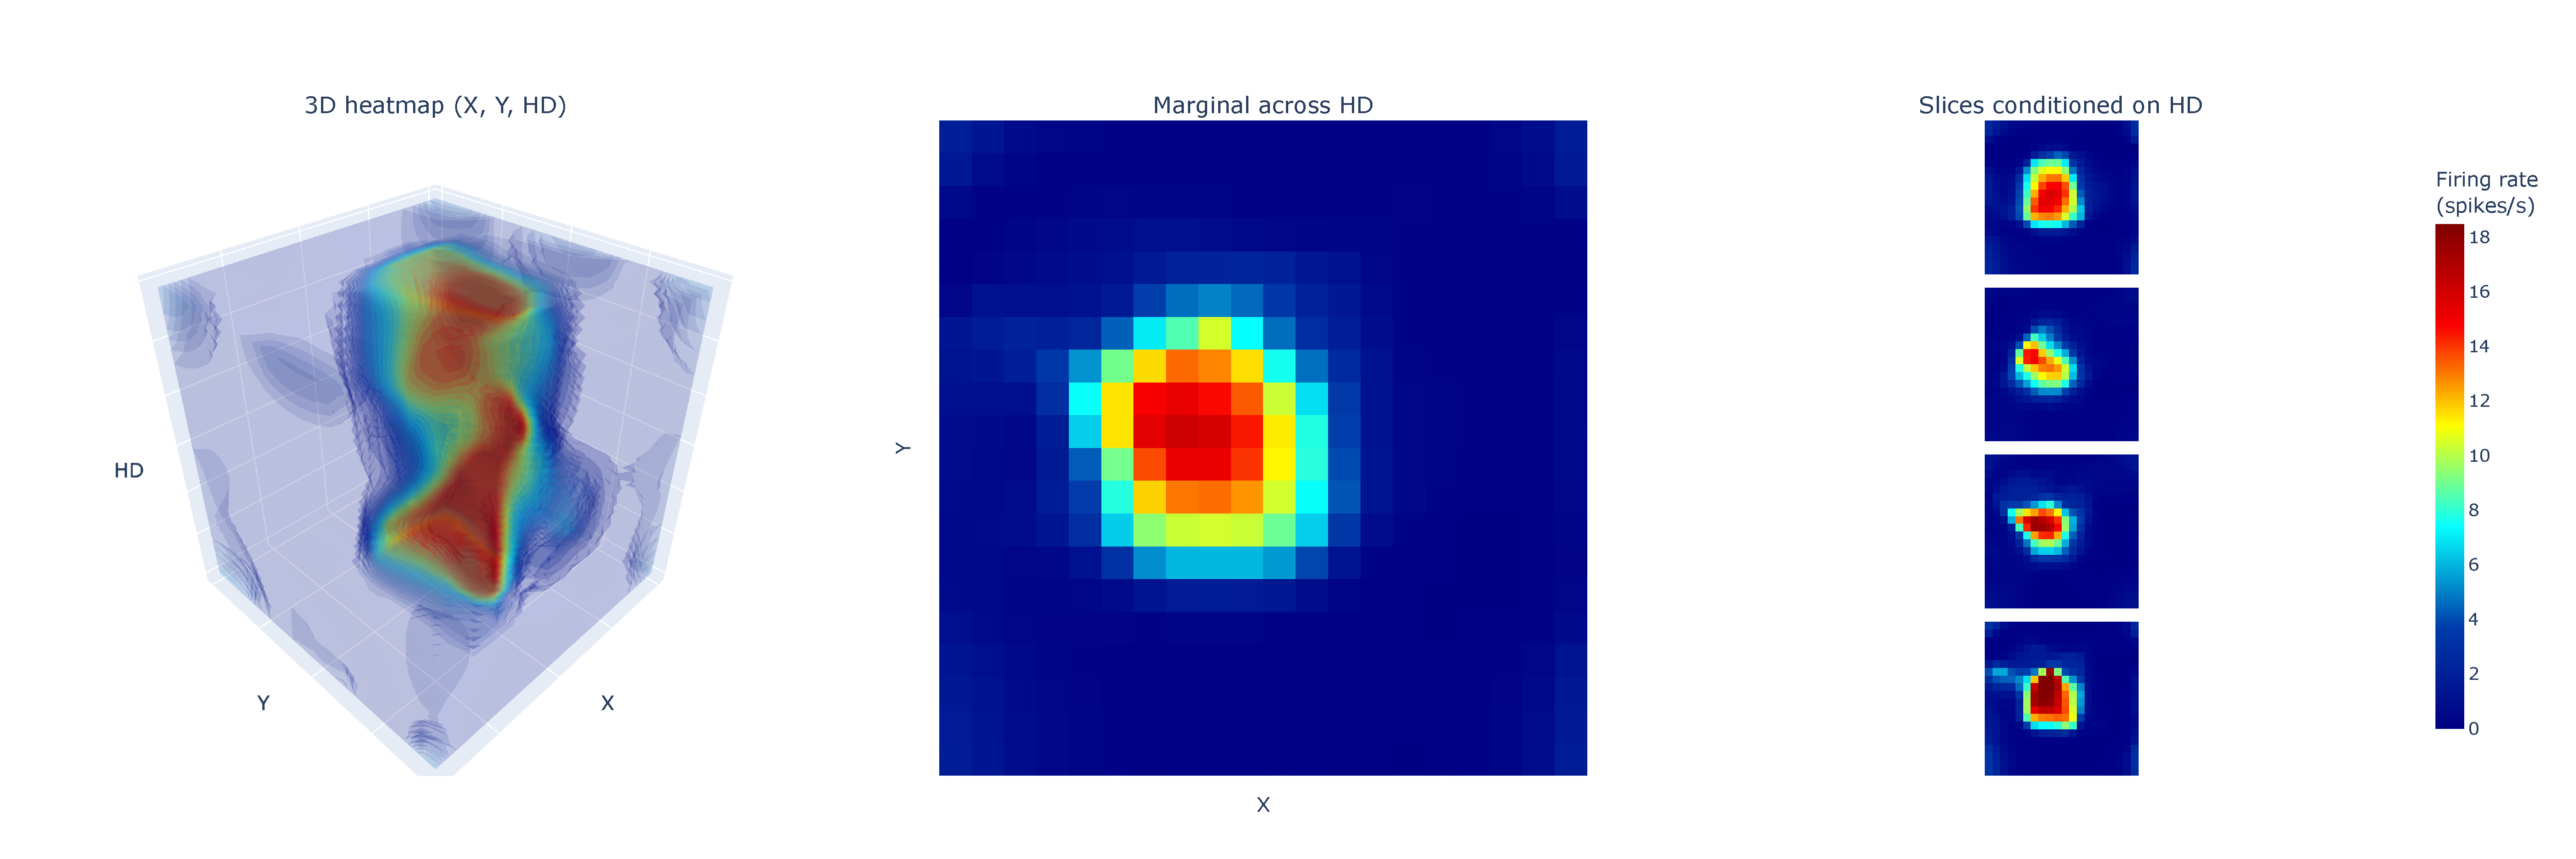
\includegraphics[width=0.8\textwidth]{figs/pfeiffer_example_xy_rank1_rat4_N63.pdf}}\\
    \subfigure[]{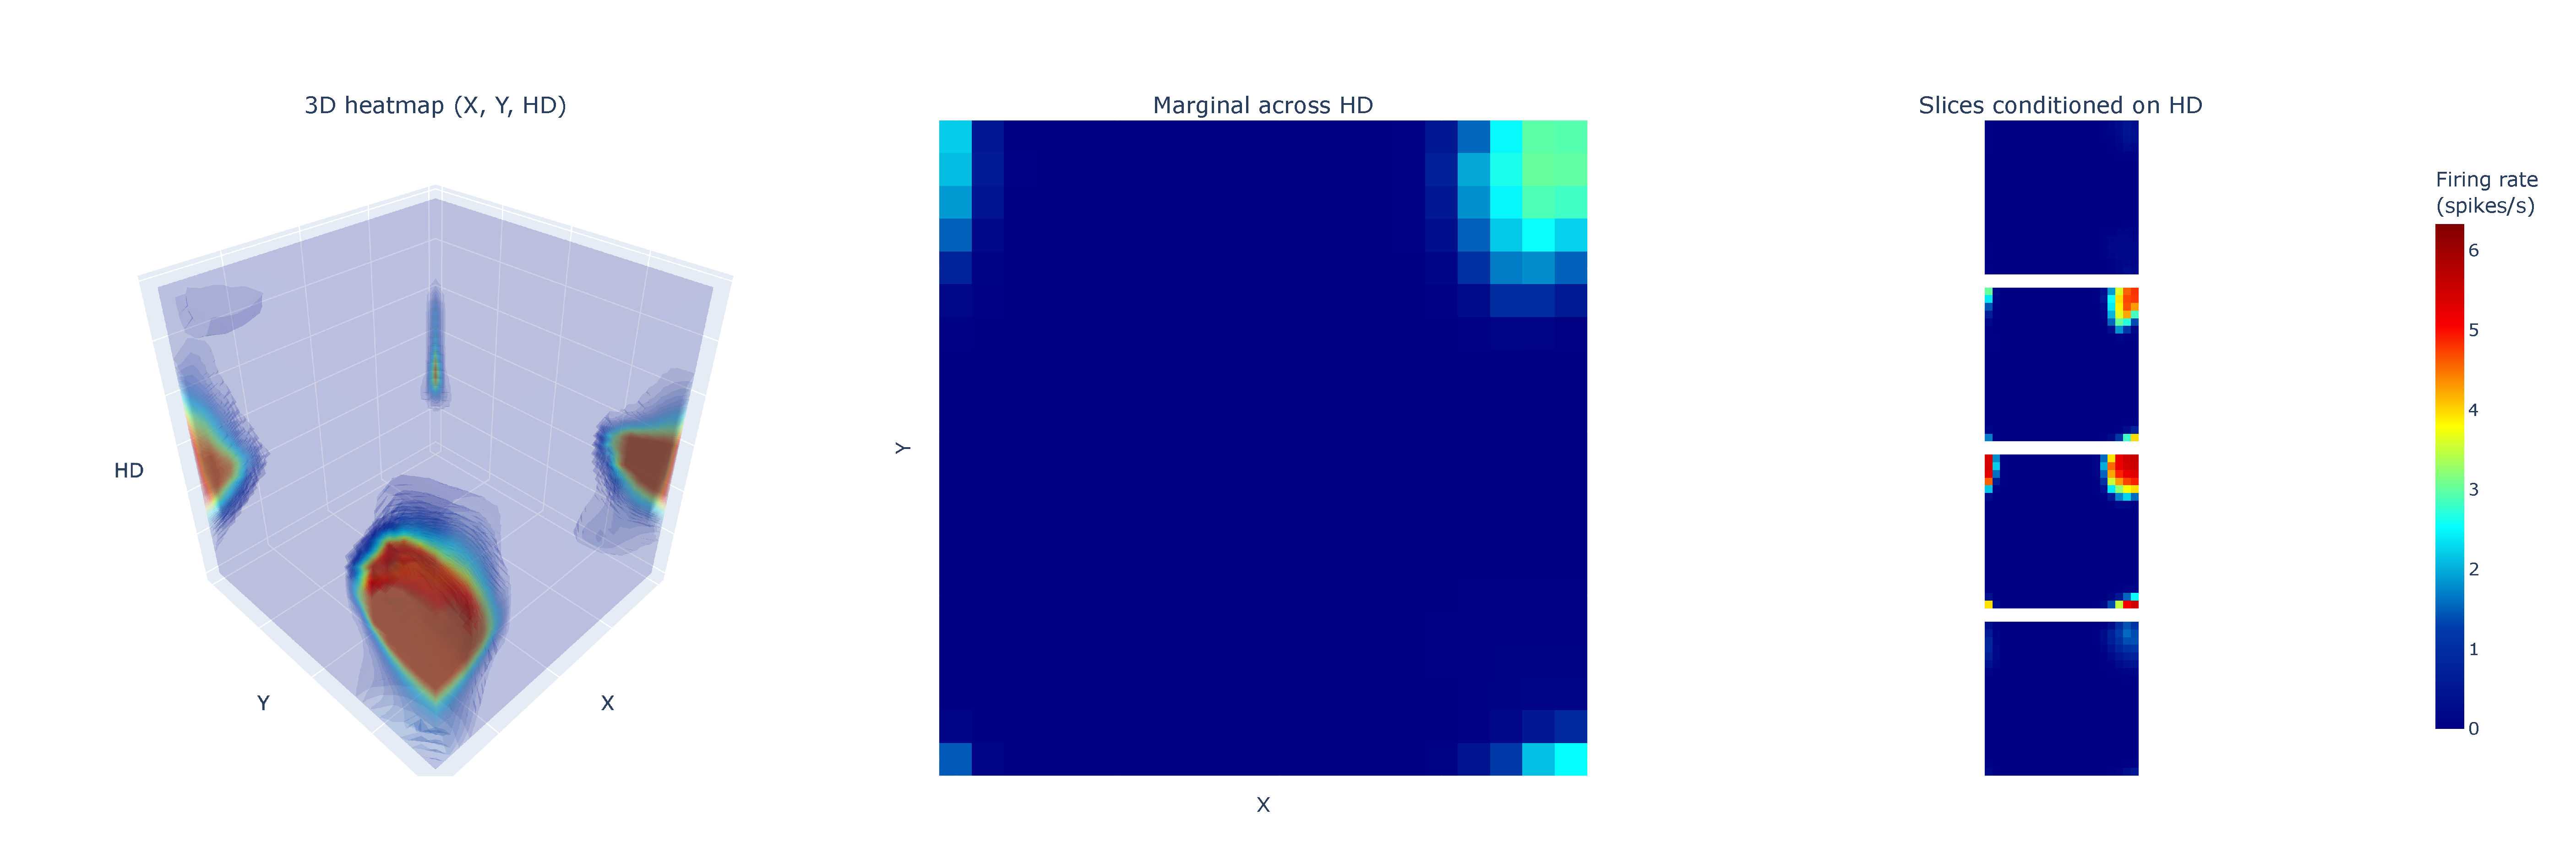
\includegraphics[width=0.8\textwidth]{figs/pfeiffer_example_xy_rank0_rat2_N133.pdf}}\\
    \subfigure[]{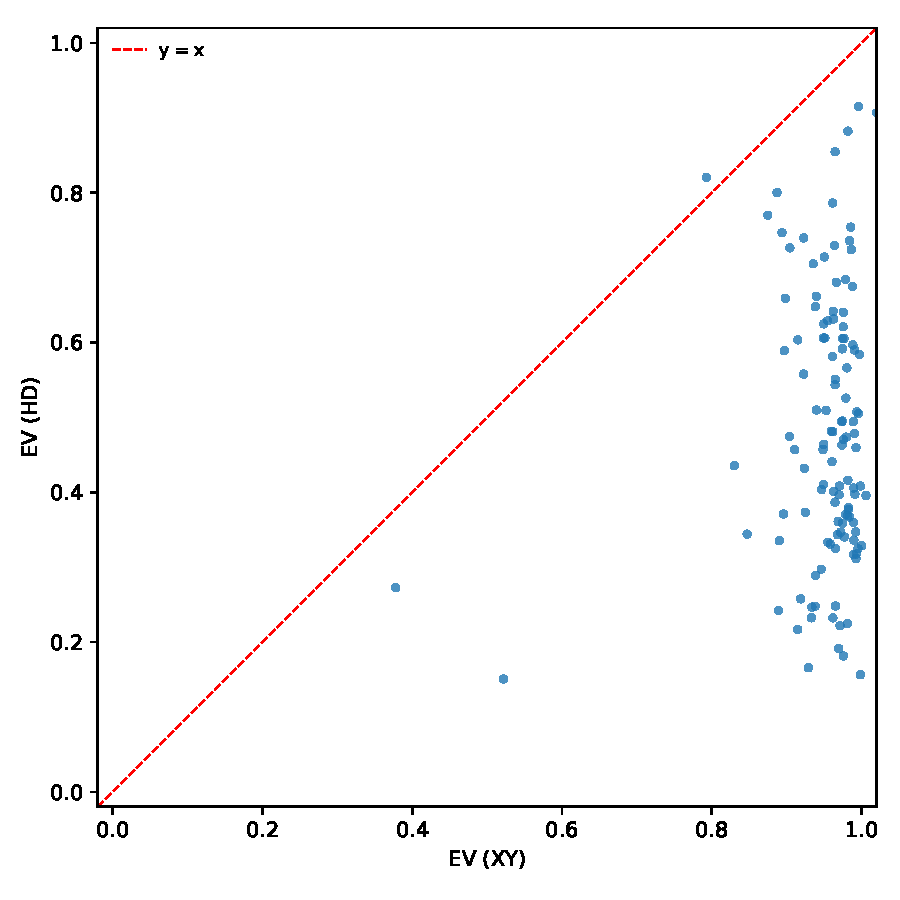
\includegraphics[width=0.25\textwidth]{figs/pfeiffer_ev_total_best_fit-corr.pdf}}\hspace{0.02\textwidth}
    \subfigure[]{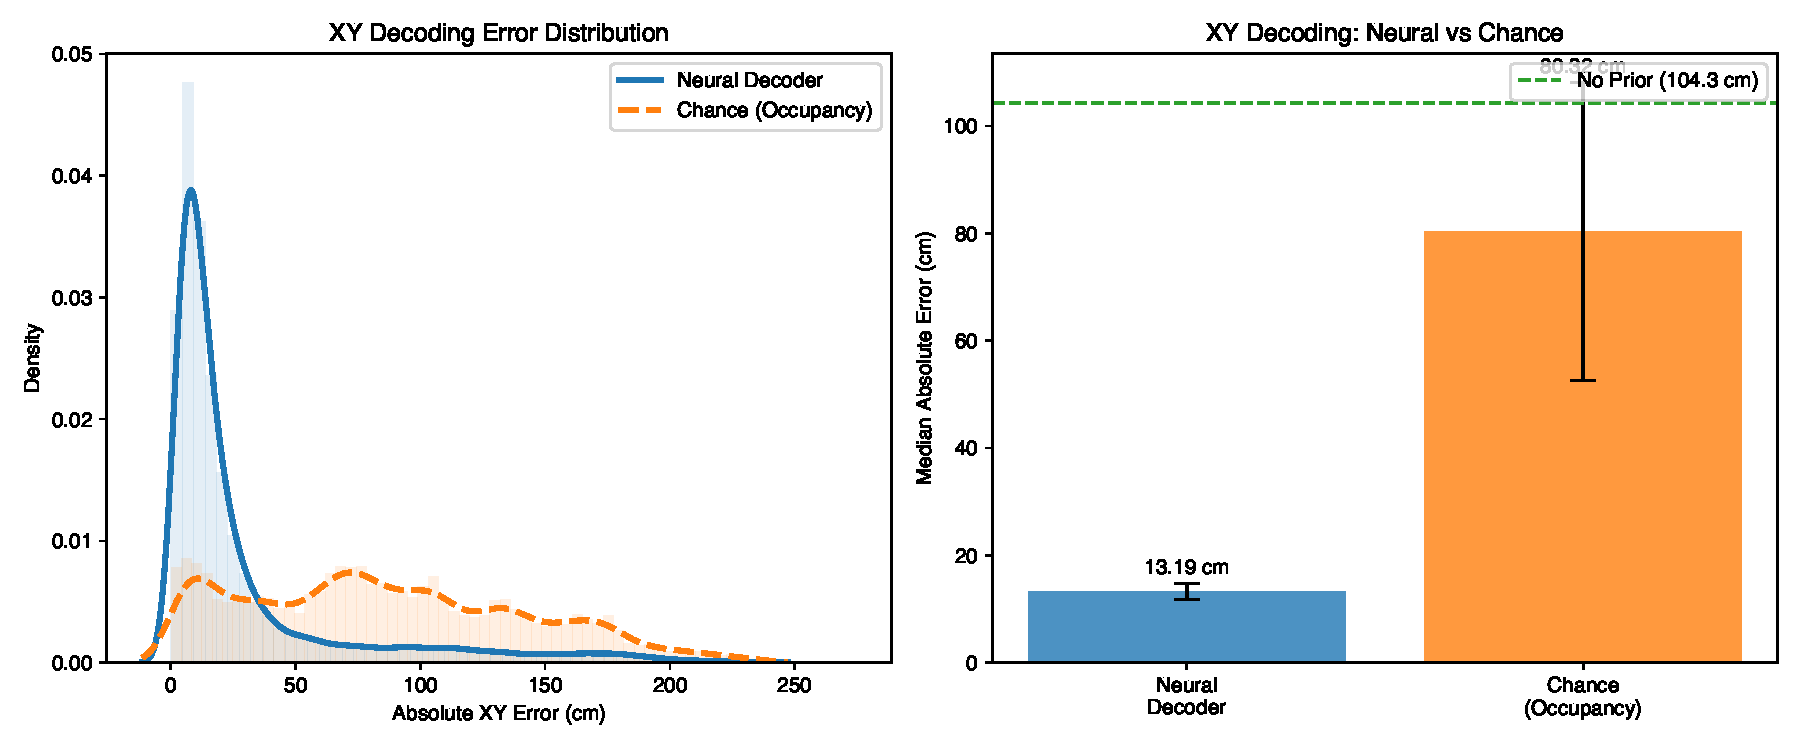
\includegraphics[width=0.34\textwidth]{figs/pfeiffer_xy_decoding_vs_chance.pdf}}
    \subfigure[]{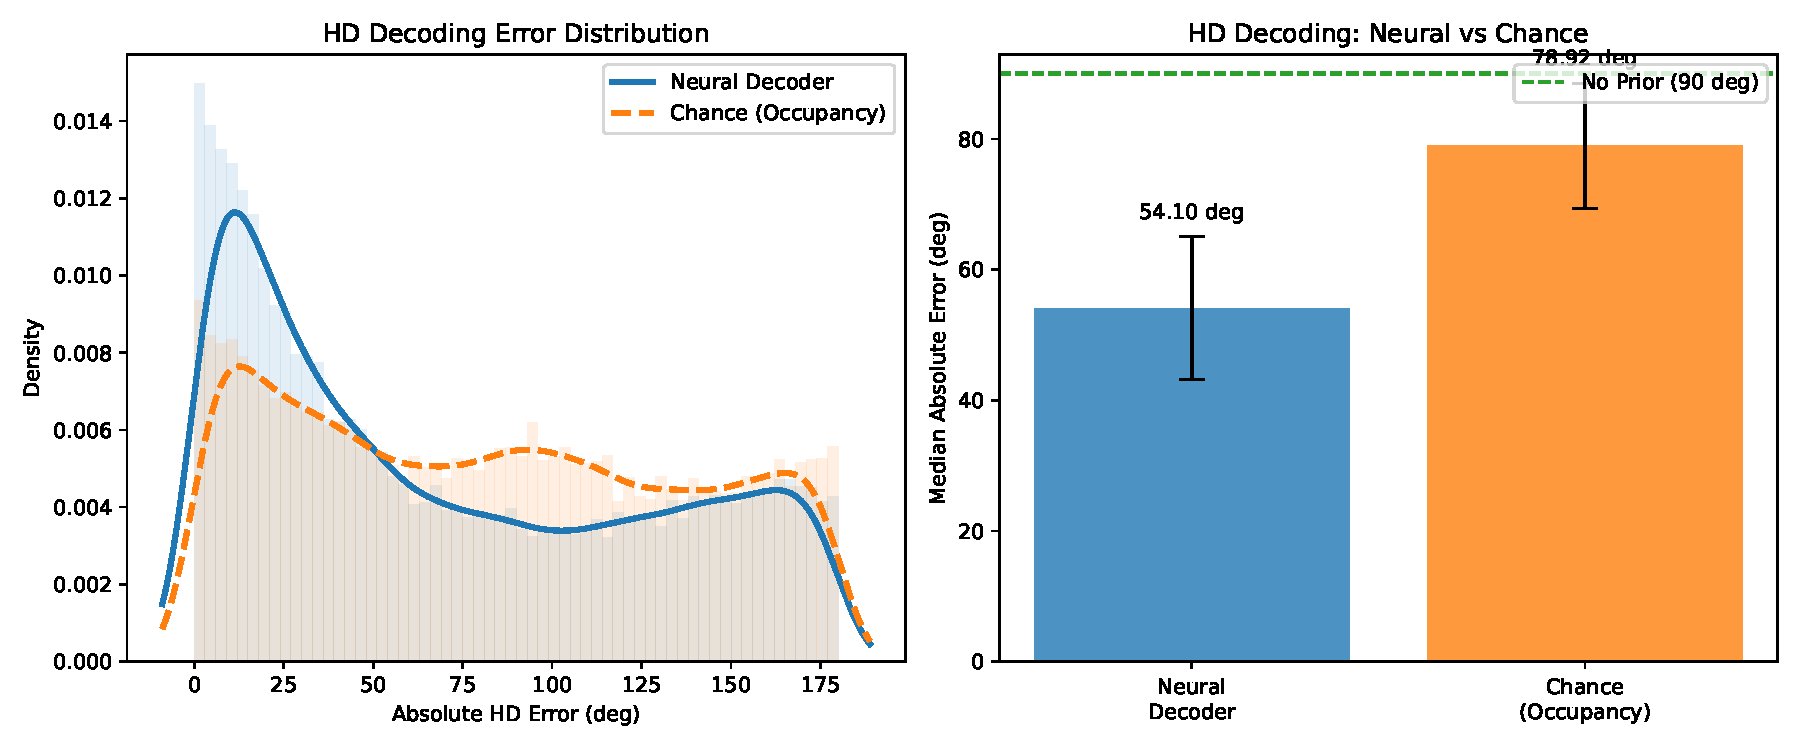
\includegraphics[width=0.34\textwidth]{figs/pfeiffer_hd_decoding_vs_chance.pdf}}
    \caption{\textbf{Place cells in the rat hippocampus are selective to locations and largely invariant to head direction.} (a) An example place cell (rat 4). Left: the joint tuning map over 2-D location and head direction rendered as a 3-D volume. Middle: the 2-D place field obtained by averaging across HD. Right: location tuning conditioned on four head-direction quadrants. The place field occupies the same location at every head direction, indicating invariance to HD. (b) Same as (a) for a second place cell (rat 2). (c) Variance explained by location ($\mathrm{EV}_{xy}$) versus head direction ($\mathrm{EV}_{hd}$) for individual place cells (30 randomly chosen cells per rat shown; $n=551$ cells from 4 rats in total), estimated with the cross-fold correlation method. The dashed line marks $\mathrm{EV}_{xy}=\mathrm{EV}_{hd}$; $99\%$ of cells lie below it. (d) Decoding of 2-D location from the simultaneously recorded population (blue) compared with an occupancy-matched chance decoder (orange): location can be accurately decoded. (e) Same for head direction: HD can not be accurately decoded from the place cell population. Chance level for uniform random guessing of HD is $90\degree$.
    }
    \label{fig:PlaceCell}
\end{figure}

%\textcolor{red}{Add a figure on 3-D tuning curves of place cells, and add a figure to quantify variance explained by place and HD }

%We performed two additional visualization. First, we plot the joint tuning for HD and x-axis of the 2-D environment. This analysis projects the 3D data onto 2-D subspace defined by HD and x-axis of location. If the neuronal response is invariant to HD, the heatmap should be dominated by vertical bar/stripe. This is indeed true for most neurons that were classified as place cells according to standard procedures used for analyzing place cells. Fig.~\ref{fig:PlaceCell}a,b show a couple of example place cells from this dataset. The vertical bar pattern is apparent when we examine the joint tuning of HD and the x-axis in 2-D environment. Similar results hold when examining the joint tuning for HD and y-axis of the 2-D environment.

%Second, we reduce the number of HD bins into 4 (each bin corresponds to one quadrant). For each HD bin, we computed the 2-D spatial firing rate map. Fig. XX shows one example neuron. As can been seen from the plots, the 2D place fields under different HD directions are highly consistent. We quantify the correlation between the different maps, and find the correlation to be... [Perform some quantification] We reason that the deviation from a perfect correlation is due to noise in the neural response. If this is the case, we expect that the correlation between spatial maps conditioned on different HD should be dependent on the firing rate of the neuron. Examining the relationship between the correlation values of maps and the firing rate, we find that ...

We quantify the contribution of HD and 2-D spatial location using the procedure developed earlier (see Fig.~\ref{fig:estimation}). 
%In particular, we are interested in whether it is indeed true that place cells exhibit invariant response to the animal's head direction. 
Fig.~\ref{fig:PlaceCell}c shows that the neural response variability is mostly explained by the animal's location: across $n=551$ place cells from four rats, location explained more variance than head direction (HD) for $99\%$ of cells (median $\mathrm{EV}_{xy}=0.97$, median $\mathrm{EV}_{hd}=0.49$). The residual $\mathrm{EV}_{hd}$ has two sources. Part of it is the finite-sampling floor of the split-half estimator, which is substantial at the fine HD binning used here (the reliability of the HD-conditioned maps, $\langle C_{ii}\rangle$, is well below 1; see Supplementary Fig.~\ref{fig:si_floor} for how this floor scales with binning and sample size); the remainder reflects a modest but genuine modulation of the gain of the place fields by head direction, visible in the conditioned slices of Fig.~\ref{fig:PlaceCell}a,b. Either way, the contribution of HD is much smaller than that of location.


To corroborate these results, we perform additional decoding analysis based on simultaneously recorded place cell populations. We found that the decoding error for location in 2-D environment is generally small (mean absolute error 14.3~cm across $n=4$ sessions in a 200~cm arena). In contrast, the decoding error for head direction is high (mean absolute error $= 69.2\degree$, compared to a chance level of $90\degree$; $n=4$ sessions; Fig.~\ref{fig:PlaceCell}d,e). These results are consistent with low contribution of the HD based on partitioning the contribution of the neural response variability in Fig.~\ref{fig:PlaceCell}c.

\textbf{Rodent head direction cells are invariant to the animal's location} Next, we analyze the head direction cell data recorded from the postsubiculum (PoSub) of mice~\cite{Duszkiewicz2024}. %This dataset contains simultaneously recorded neurons in areas \textcolor{red}{XXX}. 
We first examine the tuning properties of individual neurons by plotting the 3-D joint tuning for the head direction and the location. Visual inspection suggests that these head direction cells are largely invariant to the location of the animal in the environment. Head direction tuning curves are similar when the animal is in different quadrants of the environment. 
Using our method to partition the variability, we find that head direction explains most of the response variability, with the location accounting for a smaller portion (Fig.~\ref{fig:HD}c): across $n=1{,}489$ HD cells from 30 sessions, $\mathrm{EV}_{hd}$ exceeded $\mathrm{EV}_{xy}$ for $94\%$ of cells (median $\mathrm{EV}_{hd}=0.92$, median $\mathrm{EV}_{xy}=0.68$). The non-negligible $\mathrm{EV}_{xy}$ largely reflects the sparse sampling of the $400\times 90$ location$\times$HD bins within a session rather than genuine location tuning (see Methods). Decoding head direction and location from simultaneously recorded populations ($n=27$ sessions) reveals a large decoding error for location (mean absolute error $= 33.5$~cm in an 80~cm environment), and small decoding error for HD (mean absolute error $= 12.6\degree$).

These results suggest that there is double dissociation of the response properties of place cells and head direction cells in rodents. The response of a place cell is strongly depends on the location of the animal, and it is largely invariant to the head direction of the animal. In contrast, head direction cells are strongly tuned to head direction, and it is only minimally modulated by the animal's location. 

%These findings have implications in terms of the computations that lead to these response properties. For example, they suggest that it is unlikely that the location selectivity in place cells originates from certain visual features in the environment, in which case place cells would be expected to depend on the head direction as well. 


{\bf Comparison of the deep network model and the rodent hippocampus} Comparing the joint tuning properties to head direction and location reveal a large discrepancy between the spatial tuning properties of model neurons and spatial cells in the brain. Model units exhibit highly entangled selectivity to head direction and location. In contrast, place cells and head direction cells show disentangled selectivity for location and head direction. Thus, these recently proposed models based on visual inputs alone are insufficient to explain the key properties 
of the space cells discovered in the brain. 
In addition, our results demonstrate the importance of examining the joint tuning of multiple variables together. Joint tuning provides a more informative signature when testing models.

%Perform decoding analysis on HD. If tuning is invariant to HD, the decoding performance should be at chance level.


\begin{figure}[h!]
    \centering
    \subfigure[]{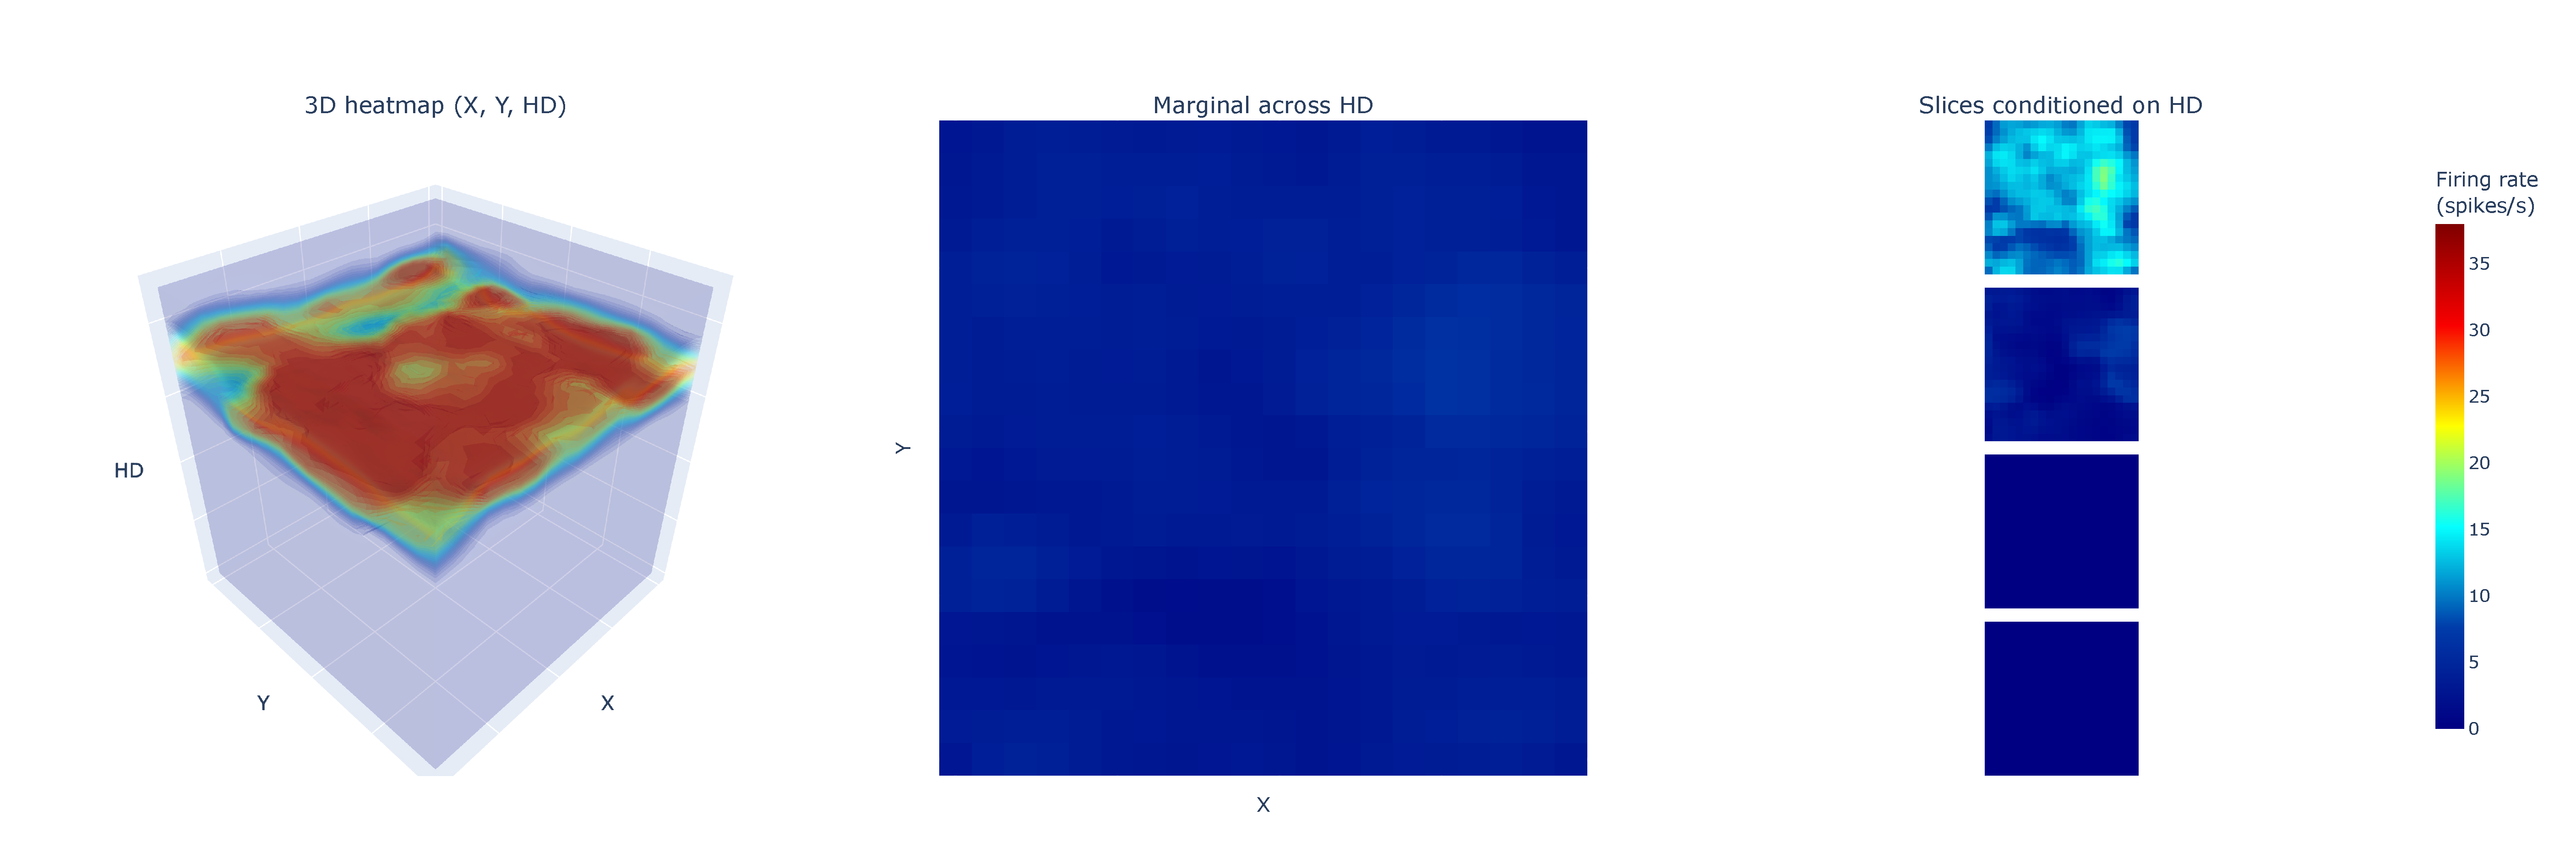
\includegraphics[width=0.8\textwidth]{figs/dusz_example_hd_rank0_A3702-191126_N13.pdf}}\\
    \subfigure[]{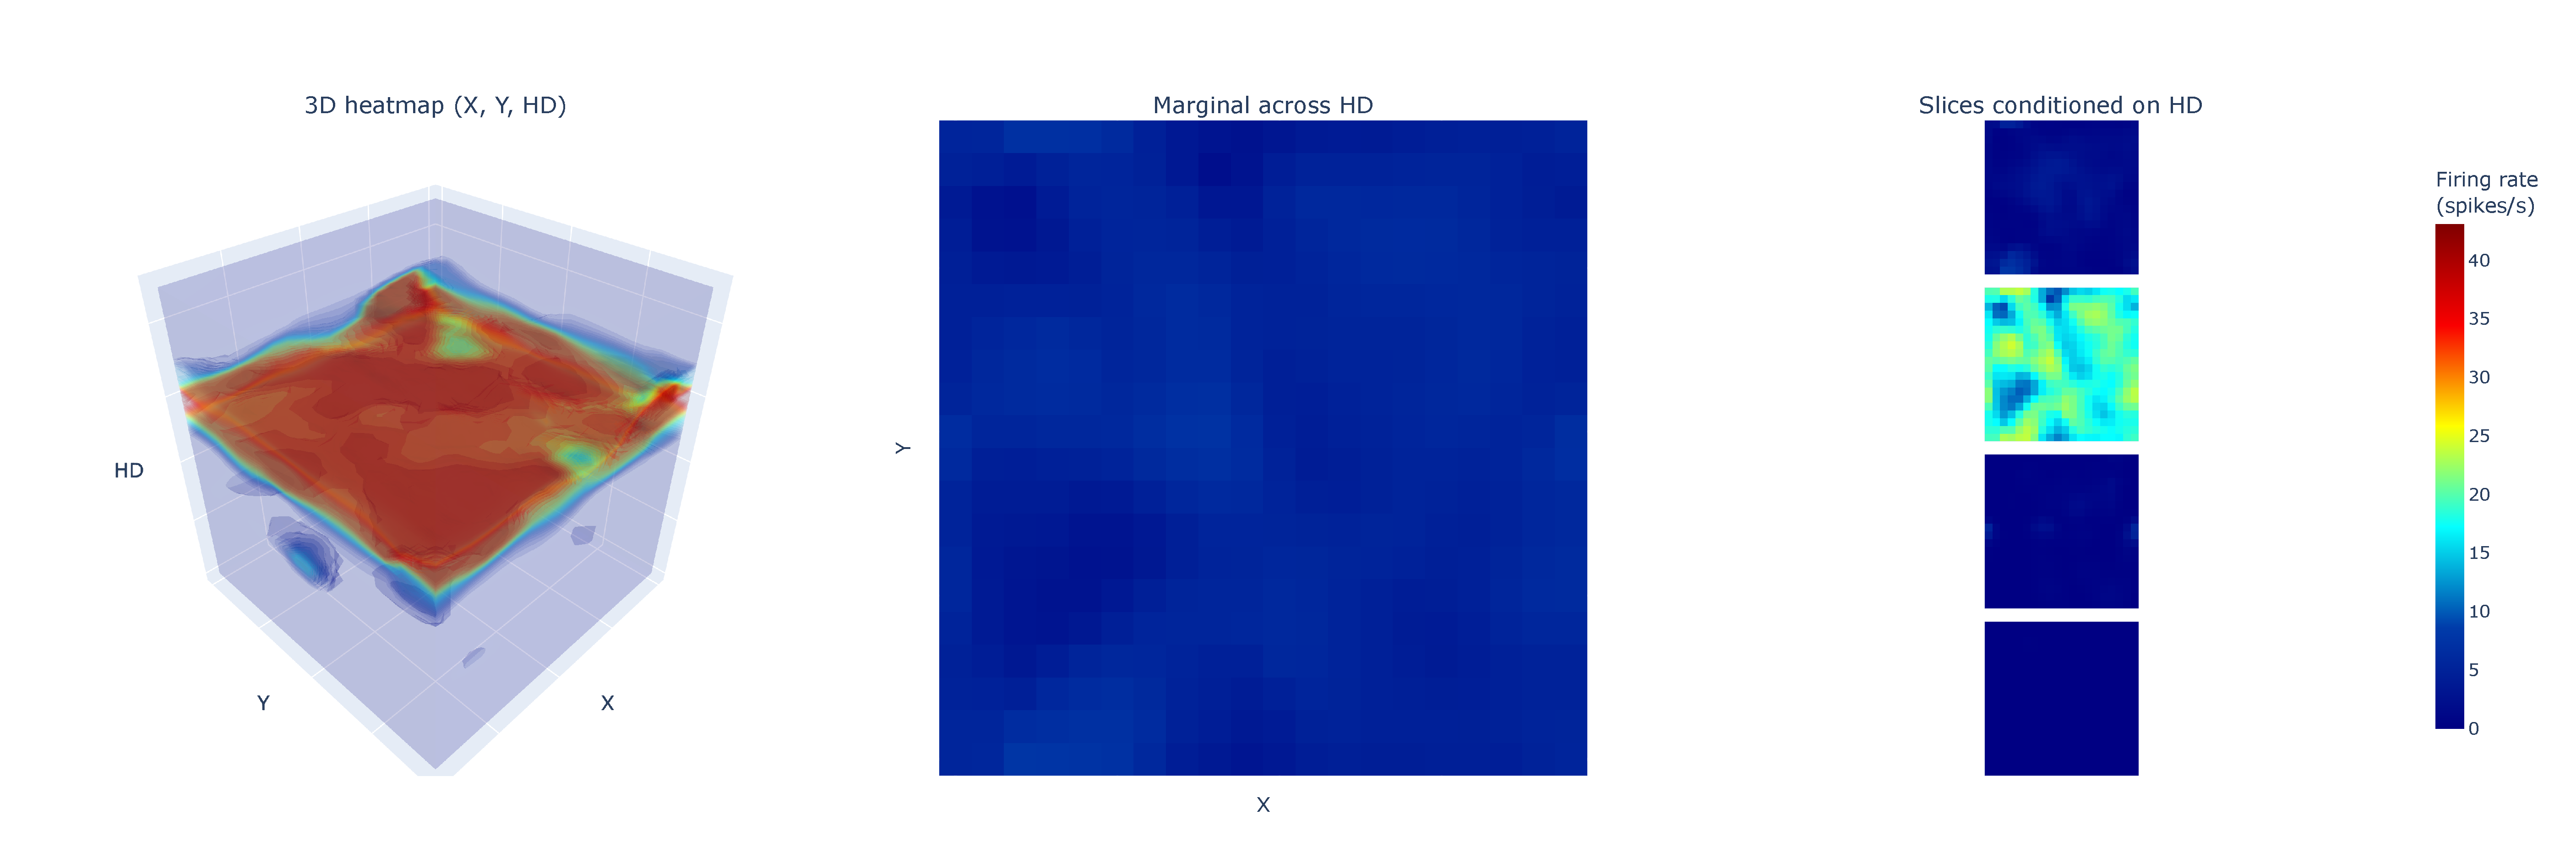
\includegraphics[width=0.8\textwidth]{figs/dusz_example_hd_rank1_A3710-200609_N57.pdf}}\\
    \subfigure[]{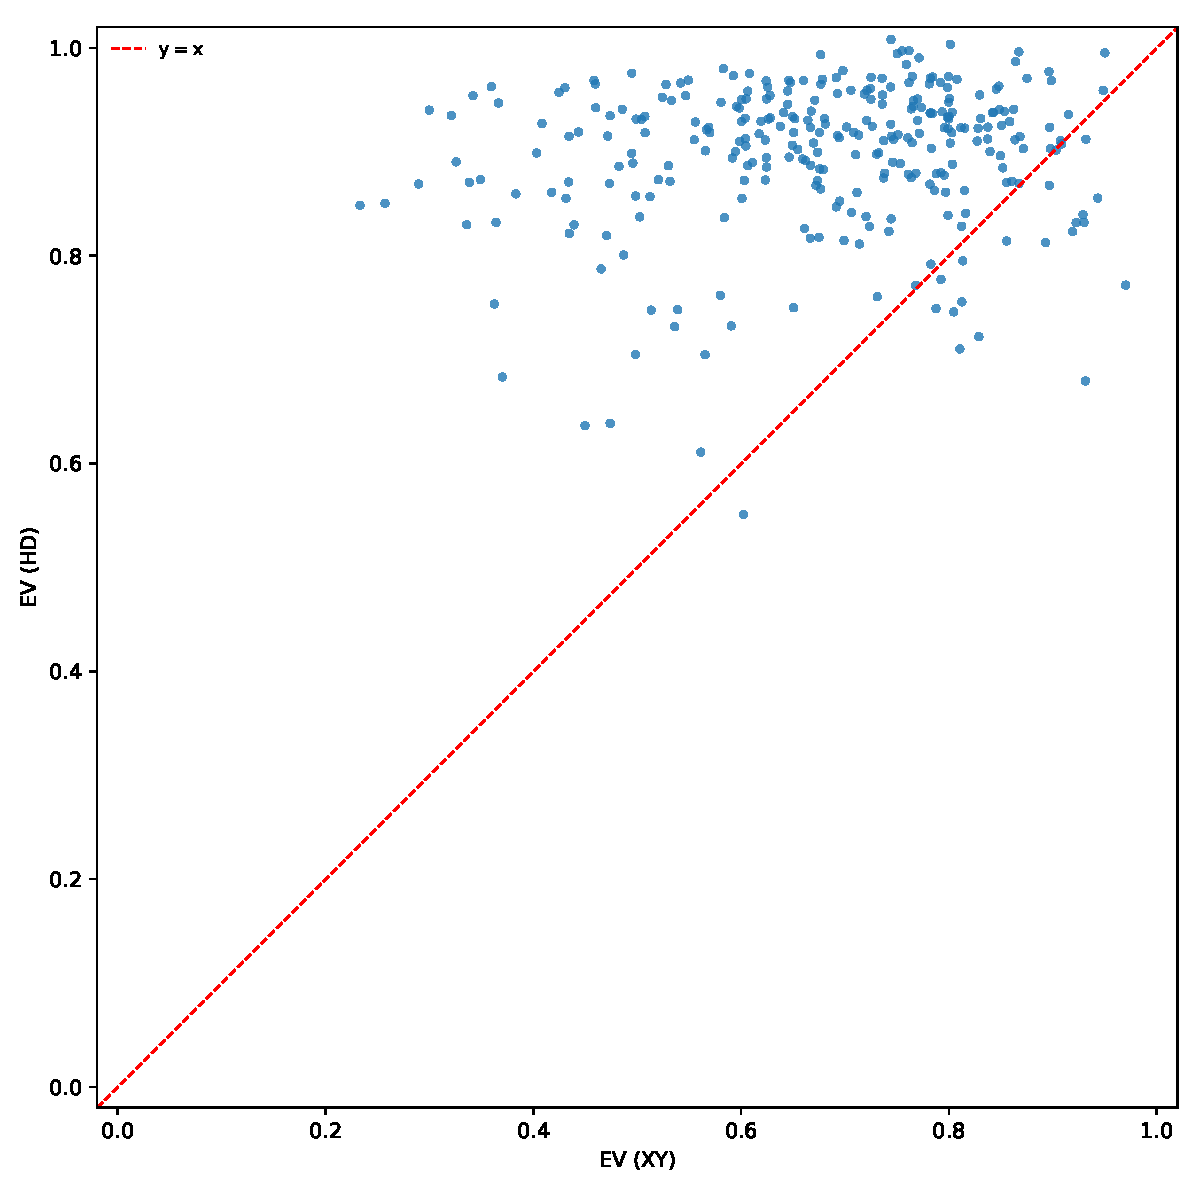
\includegraphics[width=0.25\textwidth]{figs/dusz_xyhd_ev_total_best_fit-corr.pdf}}\hspace{0.02\textwidth}
    \subfigure[]{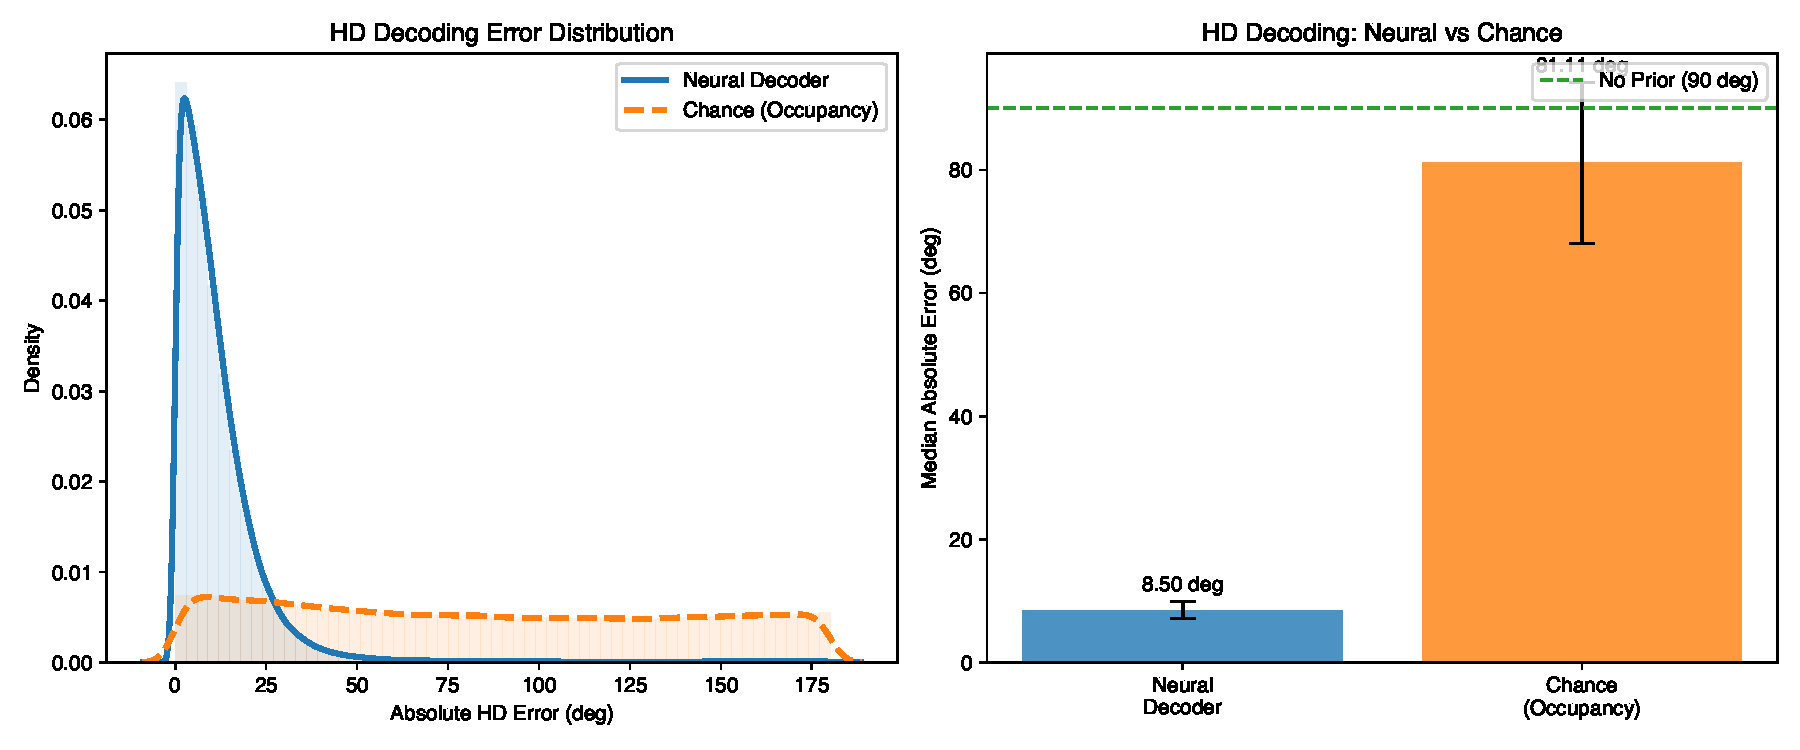
\includegraphics[width=0.34\textwidth]{figs/dusz_hd_decoding_vs_chance.pdf}}
    \subfigure[]{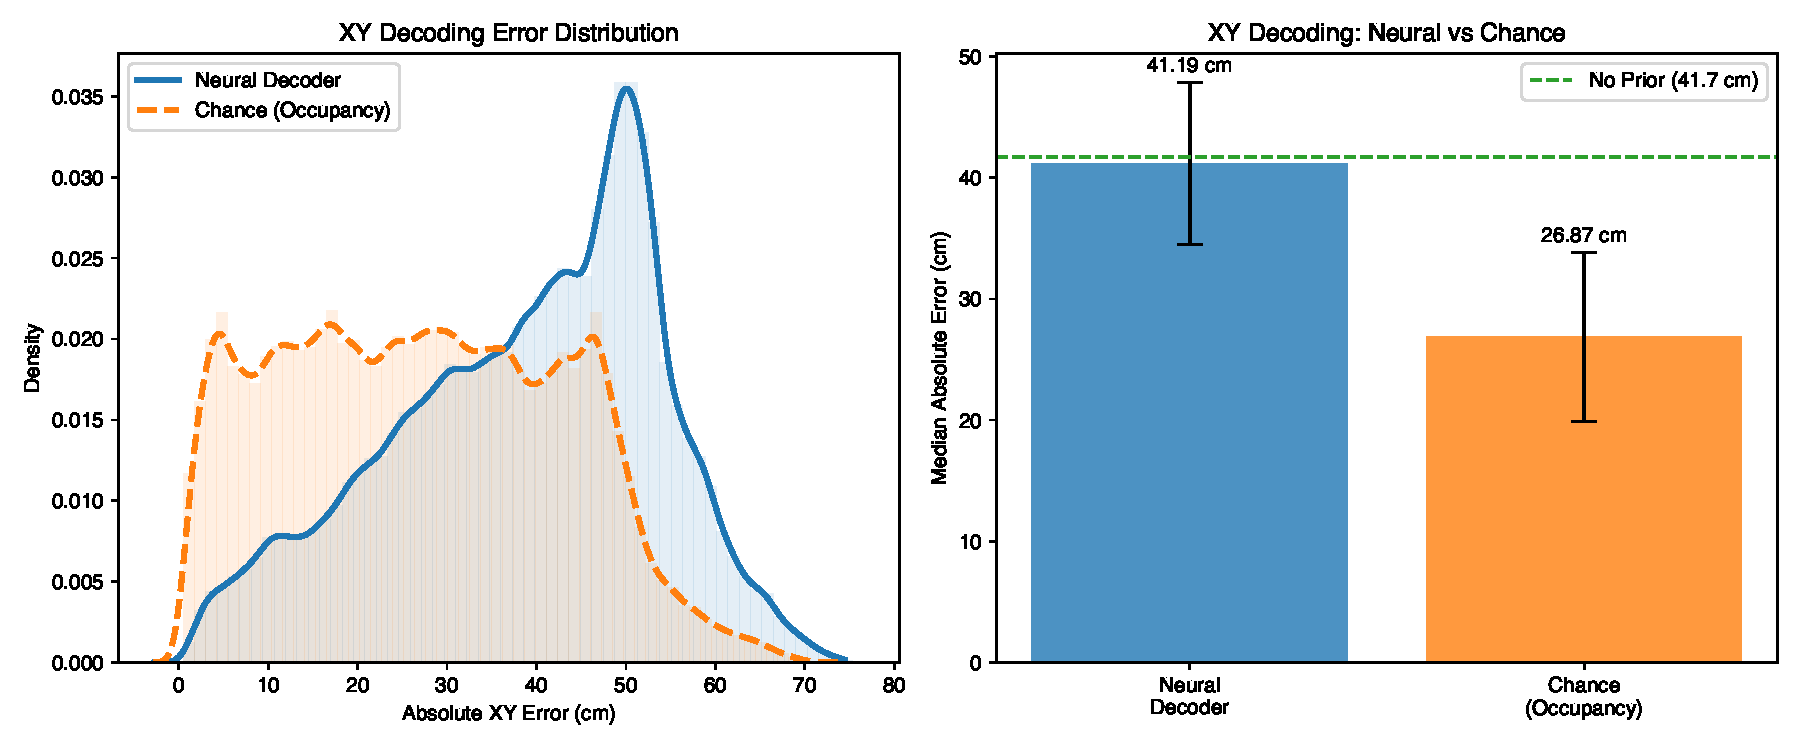
\includegraphics[width=0.34\textwidth]{figs/dusz_xy_decoding_vs_chance.pdf}}
    \caption{\textbf{Head direction cells in the mouse postsubiculum are selective to head direction, and are largely invariant to location.} (a,b) Two example HD cells, shown as in Fig.~\ref{fig:PlaceCell}a,b: the joint location$\times$HD tuning volume (left), the location map averaged across HD (middle), and location maps conditioned on four HD quadrants (right). Activity fills the whole arena at the preferred head direction and is absent elsewhere, i.e., the HD tuning does not depend on location. (c) Variance explained by location versus head direction for individual HD cells (10 randomly chosen cells per session shown; $n=1{,}489$ cells from 30 sessions in total); $94\%$ of cells lie above the diagonal. (d) Decoding of head direction from the simultaneously recorded HD-cell population compared with an occupancy-matched chance decoder. (e) Same for 2-D location.
    }
    \label{fig:HD}
\end{figure}

%\textcolor{red}{Head direction cells contain little information about space?}

%\textcolor{red}{Add a figure on the HD decoding results}


\subsection{Head direction cells are only weakly tuned to movement direction, and thus are inadequate for providing a path integration signal }

The study of joint tuning is not limited to the comparison of deep network models and the hippocampus, and may have broad relevance to for testing other computational theories of brain functions.  As an example, we will next use our framework to study a question that is essential for understanding grid cells~\cite{Hafting2005,Stensola2012}. A popular class of computational models assumes that the hexagonal grid firing properties is the result of performing path integration~\cite{Burak2009,Mcnaughton2006,Couey2013,Cueva2018}. Crucially, this class of models requires that the grid cells receive inputs of the animal's velocity (i.e., movement direction and speed). So far, neurons that encode the animal's movement speed have been identified in EC and other areas~\cite{Kropff2015speed,Hinman2016}. However, neurons that selectively encode the movement direction have not been explicitly identified.  In prior work, it was often assumed that 
head direction and movement direction are equivalent. %As the two are highly correlated, it is tempting to consider that an accurate movement direction signal would also be encoded in head direction cells.
Although the two are highly correlated, a previous study~\cite{Raudies2015head} found that: (i) head direction was more strongly encoded in head direction cells compared to movement direction; (ii) head direction and movement direction are sufficiently distinct so that using head direction as the path integration input would be insufficient for generating grid patterns in the path integration model of grid cells. However, so far it remain unclear whether the head direction (HD) cells were tuned to the movement direction (MD) when the correlation of head and movement directions are taken into account, and whether the head direction population encodes an accurate movement direction signal that would allow accurate path integration.

To address these questions, we re-analyzed the head direction cell dataset from \cite{Duszkiewicz2024}. We first examine the marginal tuning curve for head direction and movement direction, respectively. Example neurons are shown in Fig.~\ref{fig:MD}. Indeed, we find that a substantial fraction of the head direction cells in this dataset are also tuned to MD. Despite this observation, it remains unclear whether these neurons are truly selective to MD, or alternatively, the observed marginal tuning is simply due to the correlation of MD and HD. %As shown earlier, correlated stimulus sampling may complicate the interpretation of the marginal tuning curves (see Fig.~\ref{fig:fig1}f,g).
To avoid this confounding, we examine the 2-D joint tuning of HD and MD. Fig.~\ref{fig:MD}a,b shows two example neurons. It was evident that the MD tuning when conditioned on HD is rather weak. Importantly, the joint map is well populated away from the $\mathrm{MD}=\mathrm{HD}$ diagonal: in these open-field sessions head direction and movement direction were only moderately coupled (Fig.~\ref{fig:MD}c; pooled over sessions, MD lay within $30\degree$ of HD for $25\%$ of the time above the 1~cm/s speed threshold, compared with $17\%$ expected for independent variables, rising to $\approx 40\%$ above 10~cm/s), so the conditioned tuning curves are estimated from many independent HD--MD combinations. We further use our variance partitioning method to quantify the neural response variability explained by MD and HD respectively for individual neurons. We found that, across the entire population, MD explains a minor portion of response variability: $\mathrm{EV}_{hd}$ exceeded $\mathrm{EV}_{md}$ for every one of $n=1{,}465$ HD cells from 29 sessions (median $\mathrm{EV}_{hd}=0.95$, median $\mathrm{EV}_{md}=0.18$; Fig.~\ref{fig:MD}d). 

Furthermore, we performed decoding analysis using the population response to assess how accurately that MD signal is encoded in head direction cells. We found that, while MD can be decoded with a slightly higher-than-chance level, the overall error is quite large (see Fig.~\ref{fig:MD}e).  Overall, the mean absolute error for the decoded MD across $n=27$ sessions was $71.1\degree$, only marginally below the $90\degree$ chance level for uniform random guessing.  
These results suggest that the MD signal in the head direction cells is weak and unlikely to be sufficient for accurate path integration. These results suggest that the neural signal that encodes the movement direction needed for path integration remains to be identified, at least that this signal is highly unlikely encoded in head direction cells. 




\begin{figure}[h!]
    \centering
    \subfigure[]{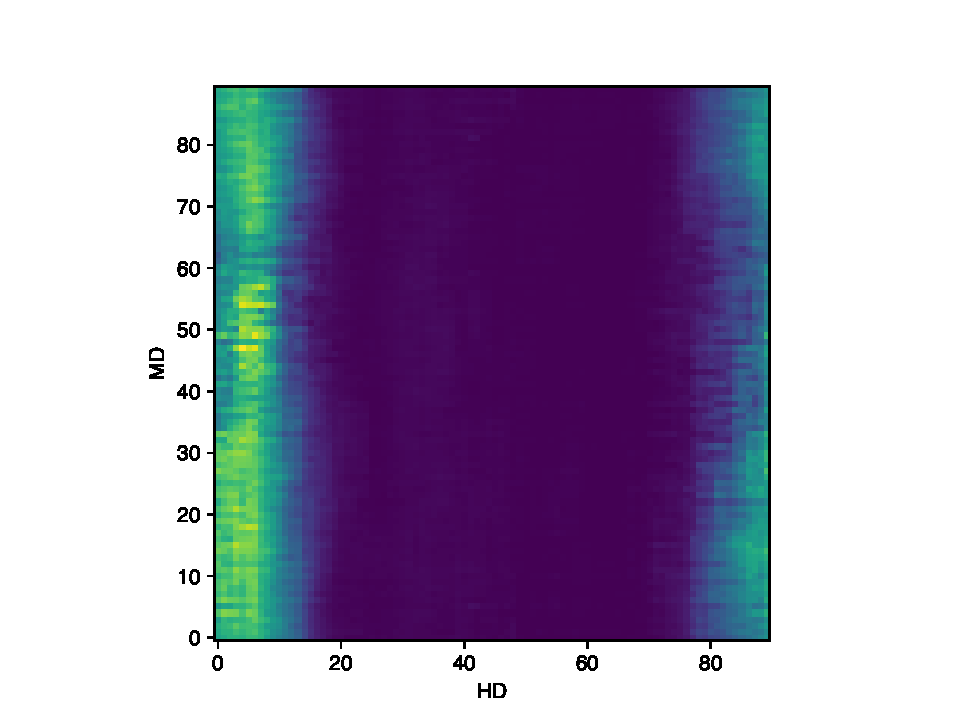
\includegraphics[width=0.31\textwidth]{figs/dusz_hdmd_D1_A3701-191119_28_joint.pdf}}
    \subfigure[]{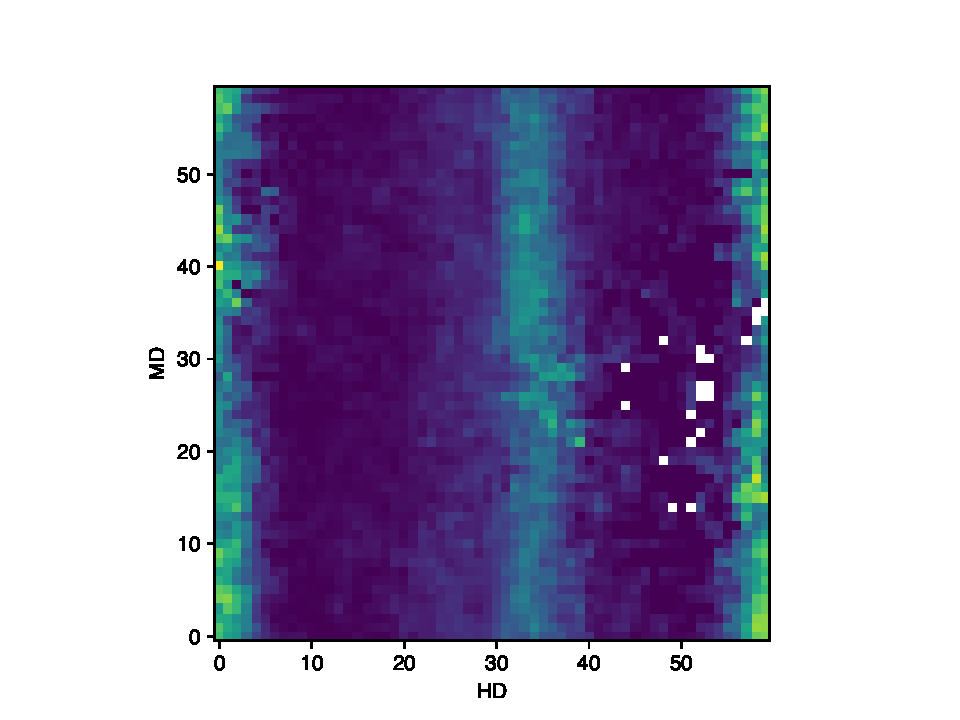
\includegraphics[width=0.31\textwidth]{figs/dusz_hdmd_D1_A3711-200810b_16_joint.pdf}}
    \subfigure[]{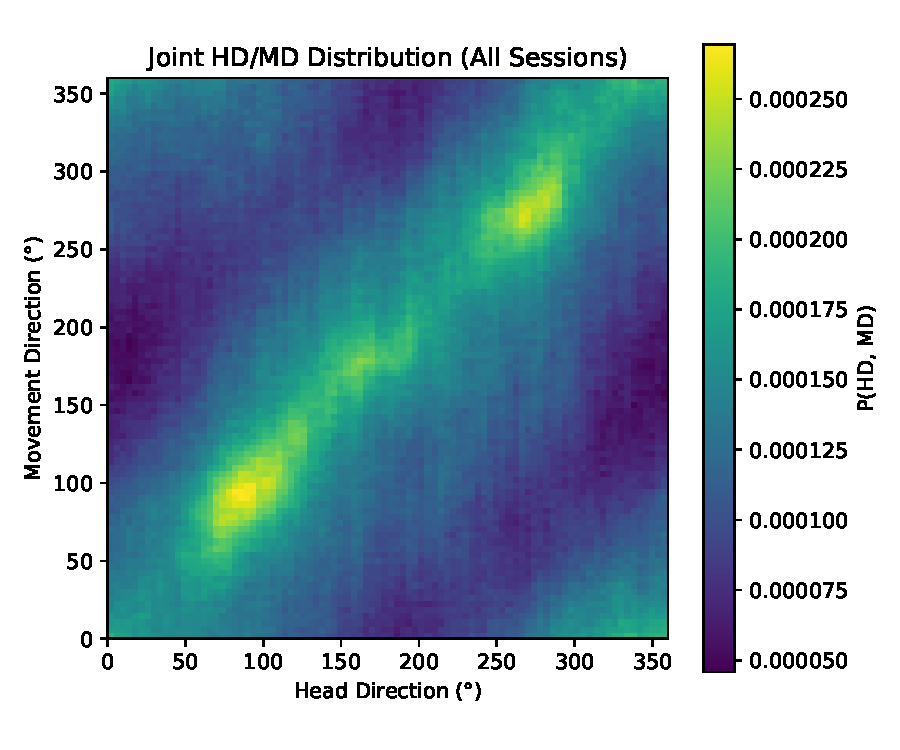
\includegraphics[width=0.31\textwidth]{figs/hdmd_occupancy_all-corr.pdf}}\\
    \subfigure[]{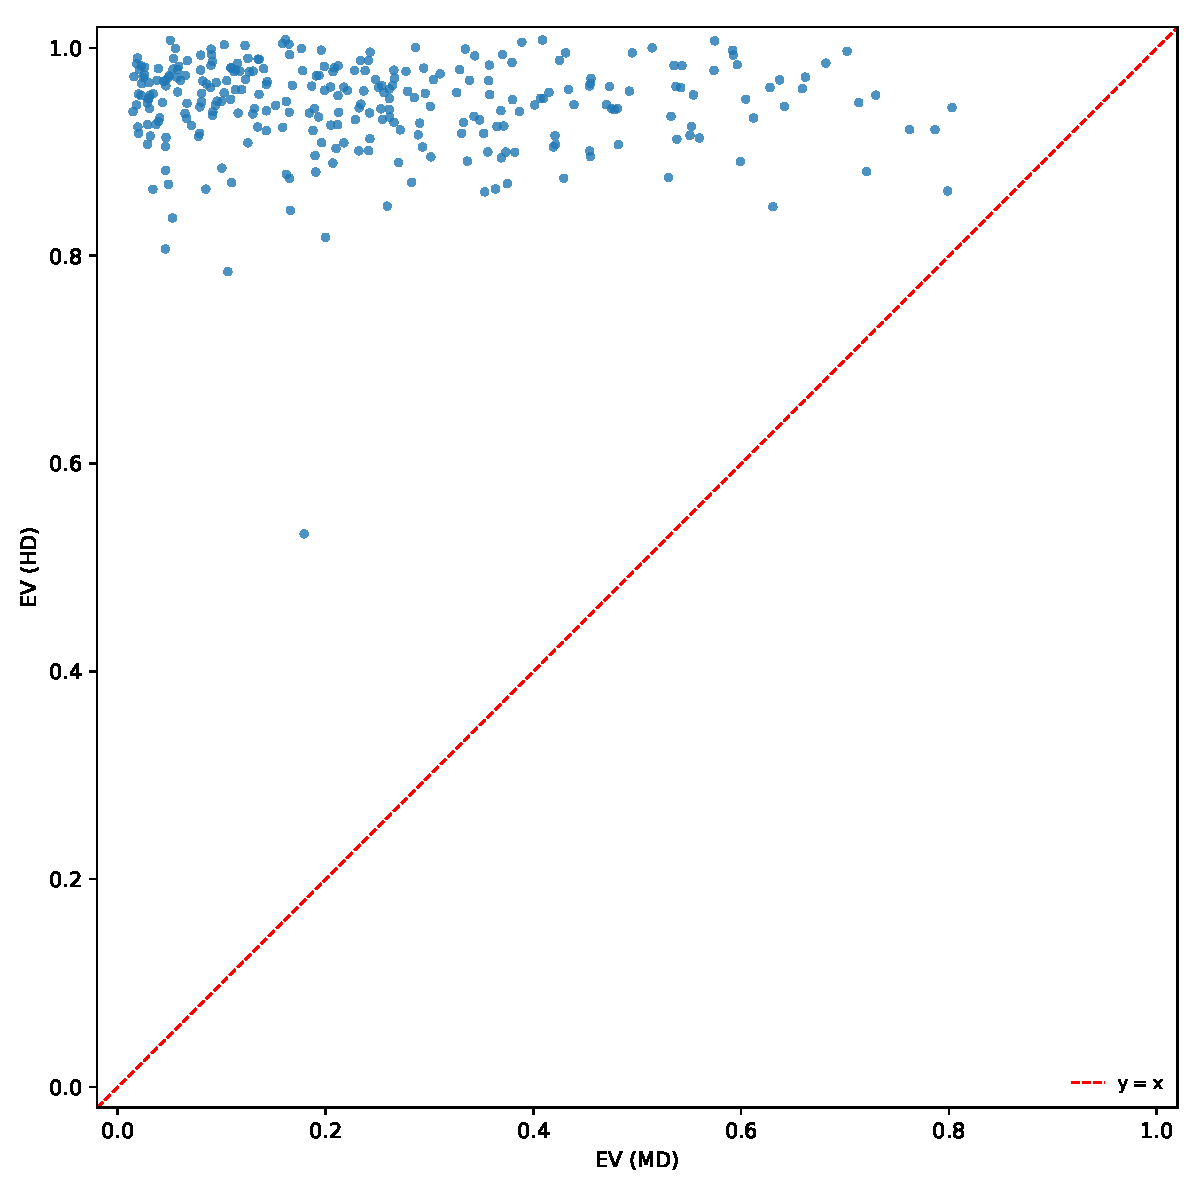
\includegraphics[width=0.28\textwidth]{figs/dusz_hdmd_ev_total_best_fit-corr.pdf}}\hspace{0.02\textwidth}
    \subfigure[]{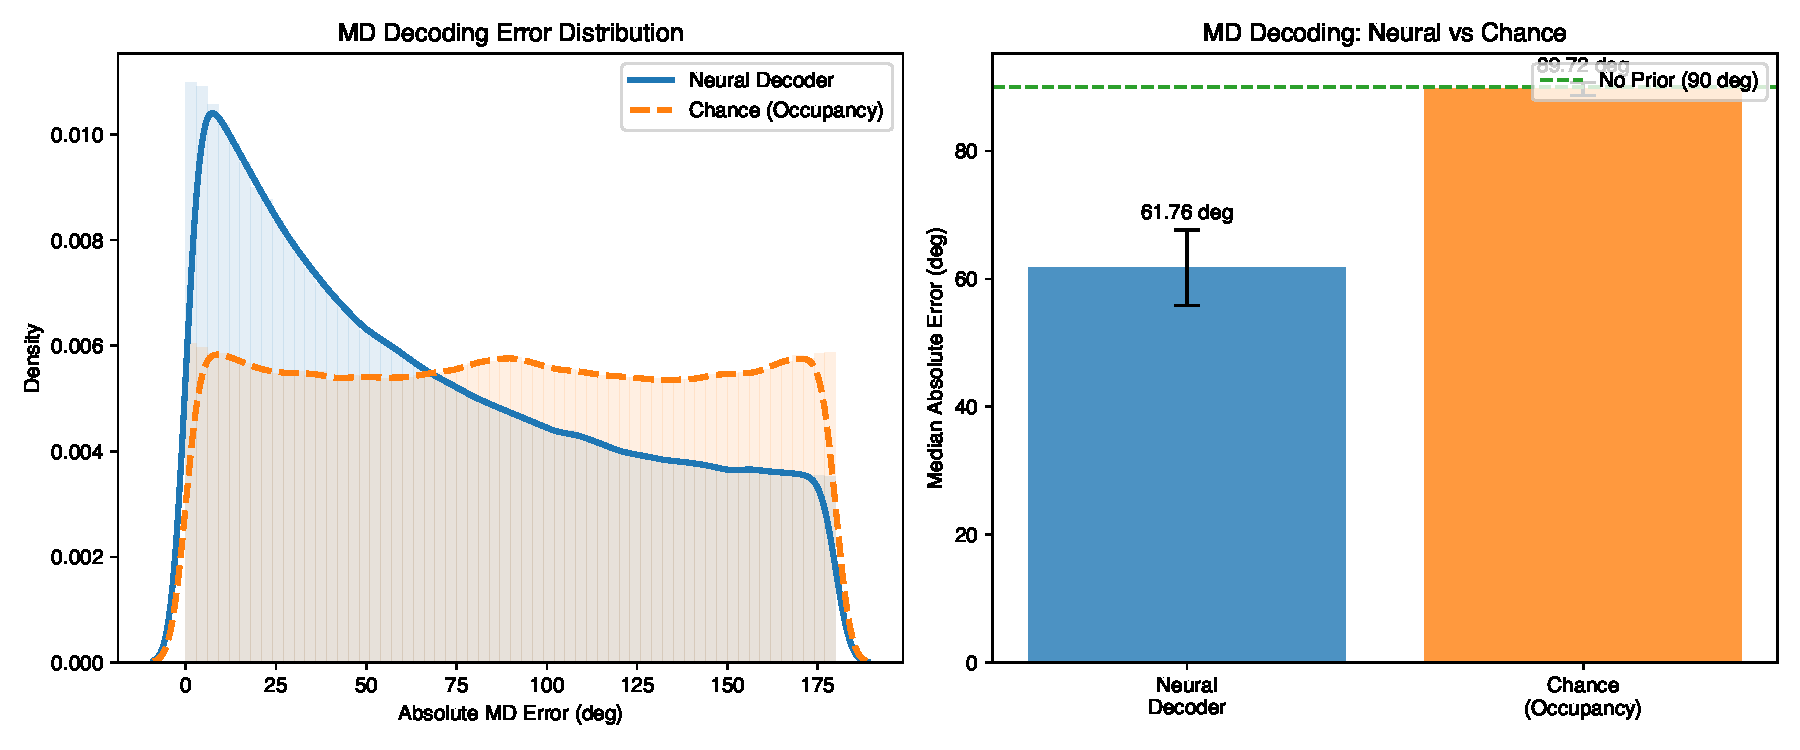
\includegraphics[width=0.6\textwidth]{figs/dusz_md_decoding_vs_chance.pdf}}
    \caption{\textbf{The MD signal encoded in the head direction population is extremely weak.} (a,b) Joint HD$\times$MD tuning maps (4$\degree$ bins) of two example HD cells. Firing is confined to a vertical band, i.e., it depends on HD but not on MD. (c) Joint distribution of HD and MD pooled over all sessions (occupancy above the 1~cm/s speed threshold). The two variables are only moderately coupled, so the joint tuning maps in (a,b) are well sampled off the diagonal. (d) Variance explained by MD versus HD for individual HD cells (10 randomly chosen cells per session shown; $n=1{,}465$ cells from 29 sessions in total); every cell lies above the diagonal. (e) Decoding of MD from the HD-cell population compared with an occupancy-matched chance decoder.
    }
    \label{fig:MD}
\end{figure}


\FloatBarrier
\section{Discussion}

% summarize the work in this paper
We demonstrate that joint tuning to multiple stimulus variables can contain critical information that is not present in the standard analysis of marginal tuning curves of individual neurons. In particular, it is important to study the selectivity and invariance of the neural code simultaneously. 
%We show that it is important to study the selectivity and invariance of the neural code simultaneously. Crucially, invariance to a certain dimension in general can not be assessed by examining the marginal tuning curve to a certain dimension. A completely flat marginal tuning curve may not mean the invariance to a certain dimension. We developed metrics to study the joint tuning by quantifying the contribution of individual stimulus variables to the response variability of individual neurons. 
%If the contribution of a variable is 0, it means that the neuron is invariant to this variable. 
%The analysis of joint tuning of a neuron to multiple stimulus variables provides more comprehensive characterizations of the neural response properties that may be missing in the analysis of tuning curves for individual stimulus variables. 
%Joint tuning is more informative for comparing the properties of different models/brain.
The joint tuning properties of individual neurons were often studied using the GLM approach~\cite{Pillow2008spatio,Hardcastle2017multiplexed}. The advantage of GLM is that it allows the partitioning of neuronal response variance based on many different variables. However, GLM assumes that joint tuning can be factorized into the product of marginal tuning of individual dimensions-- an important assumption that may be violated in practice.
%Second, the results of GLM may be difficult to interpret when the variables are correlated. 
When a large number of behavioral variables need to be considered simultaneously, GLM seems to be an effective approach as more complex models may not be able to fit to the data due to the limited sample size. However, when only a handful of variables are relevant, our proposed approach provides an powerful alternative that requires minimal assumptions, and thus may potentially reveal unique insights into the structure of the code that are not possible with GLM. 



Our investigation on the joint tuning of spatial cells in rodents reveals their selectivity and invariance. First, we find that place cells (i.e., neurons that are selective to location) are largely invariant to the head direction of the animal. While this invariance is not perfect i.e., the gain of the place fields appeared to be modulated by head direction, the location of the place fields remain stable. 
Second, head direction cells (i.e., neurons that are strongly selective to head direction) are largely invariant to location.  
%Thus, in rodents two key spatial variables (location and head direction) are represented in distinct neural populations, which supports the notion of distinct functional cell types. 
The invariance of place cells (or head direction cells) to head direction (or spatial location) suggests that the code for space is ``abstract", and is unlikely inherent from selectivity to sensory features alone. Computationally, being selective to one variable while being invariant to other variables may facilitate generalization. For example, the invariance of place cells to head direction would enable the downstream circuits to use the same decoder to extract spatial information without having to modify the readout weights according to the current head direction.





Using our approach to study neural network models developed recently based on vision tasks~\cite{Luo2024,Gornet2024automated}, we found that the tuning properties of individual neurons differ drastically from those of place cells or head direction cells in the rodent brain. %Specifically, while a faction of model units exhibit spatial selectivity, thus can be classified as putative ``place cells". These units in the deep network models do not exhibit invariant responses to HD. Instead,
Most importantly, individual units in the model encode highly entangled representation for head direction and location. In addition, most model units do not exhibit clear marginal tuning for head direction, yet their response is strongly modulated by head direction via the interaction with location. These results hold for both deep network models examined~\cite{Luo2024,Gornet2024automated}.
One interpretation is that the high entangled HD and location representation in these deep networks are due to that these neurons are selective to visual features. As these spatial variables are correlated with visual features, spatial selectivity may emerge.
%As a particular combination of head direction and location lead to the detection of certain visual features, network units would appear to be selective to particular combinations of spatial variables. 
Even a unit in an early layer of the network that essentially behaves as an edge detector might exhibit location and HD tuning.  However, such kind of selectivity observed in the model is substantially different from that of the head direction cells and place cells.
In particular, the network units are much less invariant to head direction and location compared to place cells and head direction cells in rodents.
By revealing a fundamental divergence in the response properties of model units and real neurons, 
these results reveal a major gap in current deep neural network models trained on vision tasks for explaining the tuning properties in spatial navigation systems, in particular, in rodents.  It would be interesting for future studies to determine what other ingredients would be needed for the model units to be simultaneously selective to location and invariant to head direction, as observed in rodents. It would be interesting to test whether deep neural models trained on vision tasks can better explain the neural response in primates [refs].




%While the model units show place selectivity in the marginal tuning, the lack of invariance to HD suggest that the structure of the code is fundamentally different from that of the hippocampus place cells. In these models trained on vision tasks, the encoding of head direction and location is strongly mixed at the level of individual neurons. For most individual model neurons, the contribution of head direction and location are close to equal. In contrast, in rat's brain, place cells are strongly selective to location and is only weakly selective to head direction. Head direction cells are strongly tuned the head direction, and are only weakly tuned to location. 


% discuss the importance in understanding the joint tuning property


%Our results highlight the importance of studying the joint tuning properties of neurons. The tuning properties of neurons are often studied one at a time by examining the tuning to individual stimulus dimensions. 



% we find that the head direction cells strongly encode head direction, and the movement direction signal is rather weak.
%Furthermore, we find

Our approach can be broadly applied to study the joint tuning of individual neurons to multiple behavioral variables simultaneously (ideally 2 or 3), without making additional assumptions regarding how tuning of different variables interact (such as multiplicative interactions assumed in GLM). We further demonstrated this point by studying the joint MD and HD tuning in head direction cells to show that head direction cells are largely invariant to movement direction. Thus, it is unlikely that head direction cells would encode the movement direction signal required for path integration~\cite{Mcnaughton2006}. 
Similar techniques may be used to understand the selectivity of the place cells on linear tracks with respect to location, time or distance traveled. It was proposed that hippocampal neurons on linear tracks might encode location, time, or distance traveled or a combination of these~\cite{Eichenbaum2014time,Chen2024}. Although some progress has been made, it remains challenging to disentangle the contribution of these different factors because they are highly correlated in the experiments. Our approach provides a new way to estimate the contribution of these different factors in future research. 

Our results have implications for the study of mixed selectivity of neurons~\cite{Rigotti2013}, which has been reported in various brain areas in different tasks. First, from a methodological perspective, our techniques provide a new way to quantify mixed selectivity through the examination of joint tuning and the quantification of the contribution of individual stimulus variables. Second, our results based on the analysis of spatial tuning properties of the deep network models suggest that, in some cases, mixed selectivity may arise due to the difficulty in identifying the correct feature sets or stimulus variables. For example, in the deep network models examined here, many neurons in the first layer are oriented filters, thus they encode the orientation of edges. 
%Analysis of orientation selectivity of these units would lead to a clear interpretation of their response properties. 
However, when analyzing the spatial tuning properties of these units, they exhibit complex non-linear mixed selectivity for these spatial variables. In this case, nonlinear mixed selectivity arises due to the highly nonlinear mapping between the visual feature and the spatial variables (location and head direction). Only for particular combinations of location and head direction of the agent, an edge of certain orientation would appear in the receptive field of the model unit. Empirically observed mixed selectivity in neural systems has been proposed to carry certain functional advantage in coding ~\cite{Rigotti2013,Fusi2016neurons}. The discussion above suggests that mixed selectivity could also arise due to mis-identification of the features encoded. Extra care would be needed to interpret these response patterns that appear to be mixed selective. 

%While these problems have been recognized previously. For example, in studying whether the HD cells are selective to HD or movement direction, more careful analysis were used to show that the head direction signal is more strongly encoded in these neurons~\cite{Raudies2015head}. However, so far, it was not clear collectively how strong the movement direction signal was encoded in these neurons. Through the analysis of joint tuning, in particular the selectivity to movement direction conditioned on HD, a unambiguous interpretation can be reached. Similar techniques may be used to understand the selectivity of the place cells with respect to location, time or distance traveled. 

%Generalization to the cases of many variables.





%Discuss mixed selectivity.

In this paper, we have focused entirely on the response properties of individual neurons. An interesting and important question is the implication of the selectivity and invariance observed at the neural population level. Previous theoretical work suggests that the tuning properties of individual neurons constrain the population-level properties as they define the projection of the neural manifold onto the individual neuronal axes~\cite{Kriegeskorte2021}. However, this basic question is mainly investigated in the context of encoding a single stimulus variable. Understanding the relationship between the properties of joint tuning of multivariate stimuli and the structure of the neural manifold structure represents an important direction for future research. 

%Discuss the implication of mixed code on representational geometry


% discuss the work on the model of the cognitive maps and the importance in taking the coordinate system transformation into account. 

% discuss the work on mixed selectivity

% discuss the future direction, and the limitation of current work


\newpage

\section{Methods} 

%We analyzed data from a real place cell dataset from Pfeiffer et al. and compared it against representations in deep neural network models. Our goal was to examine whether artificial neural networks can replicate spatial representations found in the brain. Several neural network models were used, including general-purpose image-processing architectures and models specifically trained to emulate spatial tasks typically considered to be the domain of the hippocampus.

\subsection{Analysis of marginal tuning curve under correlated stimulus sampling}
Here we show that how correlated sampling of the stimuli could lead to spurious tuning when using the standard analysis of tuning curves. Suppose that we consider the tuning properties of a neuron to variables $x$ and $y$. Denote the joint tuning of this neuron to $x$ and $y$ is $h(x,y)$.

Assuming the marginal sampling distribution over $x$ is uniform, the marginal tuning curve for $x$ is estimated (through the standard averaging procedure used) to be
$$
\hat{f}(x) = \int p(y|x)h(x,y)dy = \int p(y|x)f(x) g(y)dy =f(x)\int p(y|x)g(y)dy
$$

% TODO(author): decide whether an additional Methods figure is needed to illustrate the marginal-tuning confound under correlated sampling. Fig.~\ref{fig:fig1} (simulation parameters in the subsection below) already demonstrates this effect.

If random variables $x$ and $y$ are independent, the procedure recovers $f(x)\int p(y)g(y)dy$, which is proportional to $f(x)$. Otherwise, due to the interaction in the $p(y|x)$ term, in general the estimated marginal tuning curve for $x$ will be affected by $g(y)$. 
%In the extreme case that only $y=x$ is sampled, the estimated tuning curve becomes $f(x)g(x)$.

Consider a special case where the neuron is invariant to $x$, i.e., $h(x,y)=h(y)$ is a narrow Guassian function. In this case, the ground truth tuning curve to $f(x)$ should be a constant. Assuming that only $y=x$ is sampled (perfectly correlated sampling of the two stimuli), the estimated tuning curve would be
$$
\hat{f}(x) = \int p(y|x)h(y)dy = \int \delta(y-x)h(y)dy=h(x).
$$
Thus, in this case, if we rely on computing the marginal tuning curves to infer the tuning properties, we would incorrectly conclude that the neuron is strongly tuned to $x$.

\subsubsection*{Simulation parameters for marginal confound and GLM demonstrations (Figs.~\ref{fig:fig1} and \ref{fig:glm})}

For the marginal confound demonstration (Fig.~\ref{fig:fig1}), we simulated a neuron with true tuning $h(x,y) = \exp(-x^2 / 2\sigma_x^2)$ with $\sigma_x = 1.0$ (arbitrary units), so that the neuron is selective to $x$ and completely invariant to $y$. We drew $N = 300$ samples from a bivariate distribution where $x$ was sampled uniformly over $[-4, 4]$ and $y$ was drawn from a truncated normal distribution $y \sim \mathcal{N}(x, \sigma_{\mathrm{cond}}^2)$, clipped to $[-4, 4]$. Three correlation levels were tested by varying $\sigma_{\mathrm{cond}} \in \{4.8, 2.1, 0.6\}$, corresponding to weak ($\rho \approx 0$), moderate ($\rho \approx 0.6$), and strong ($\rho \approx 0.9$) correlation. Marginal tuning curves for $y$ were computed by binning into 30 bins and smoothing with a Gaussian kernel ($\sigma = 1$ bin). Bins with fewer than 5 samples were excluded.

For the GLM demonstration (Fig.~\ref{fig:glm}), we simulated Poisson neurons with firing rates governed by a rotated Gaussian: $\lambda(x,y) = \exp(\alpha - u^2 / 2\sigma_u^2)$, where $u = x \cos\theta - y \sin\theta$ is a rotated coordinate, $\alpha = \log 5$, $\sigma_u = 1.2$, and $\theta \in \{45\degree, 60\degree\}$. Stimuli $x$ and $y$ were drawn independently from $\mathcal{N}(0, 1)$ with $n = 20{,}000$ samples. Spike counts were generated from a Poisson distribution with rate $\lambda(x, y)$. A quadratic Poisson GLM of the form $\log \lambda = \beta_0 + \beta_1 x + \beta_2 y + \beta_3 x^2 + \beta_4 y^2$ was fit using maximum likelihood. The GLM predictions for $f(x)$ and $g(y)$ were obtained by evaluating the fitted model along each axis while holding the other variable at its mean value.

\subsection{Estimating the contribution of individual stimulus variables to neural response variability}
We first split the data evenly into two folds. Suppose that we compute the joint firing rate map for variables $x$, $y$ using each fold, denoted as $f^{(0)}(x,y)$ and $f^{(1)}(x,y)$, respectively. Further suppose that we discretize $x$ and $y$ into $m$ and $n$ bins respectively, writing $f^{(0)}_{i,j} = f^{(0)}(x_i, y_j)$ and $f^{(1)}_{i,j} = f^{(1)}(x_i, y_j)$.

To quantify the contribution of $x$, we ask how much the neuron's tuning over $y$ changes across different values of $x$. For each bin $x_i$, we extract a one-dimensional tuning curve over $y$ by fixing $x = x_i$. We denote these slices as $\mathbf{f}^{(0)}_i = f^{(0)}(x_i, \cdot)$ and $\mathbf{f}^{(1)}_j = f^{(1)}(x_j, \cdot)$ for the two folds, where each is a vector of length $n$. This approach captures joint effects: even when the marginal tuning to $x$ is flat, it will detect cases where $x$ modulates the response through its interaction with $y$.

We then compute the cross-fold Pearson correlation between every pair of these tuning curves:
\begin{equation}
C_{ij} = \mathrm{corr}\!\left(\mathbf{f}^{(0)}_i, \; \mathbf{f}^{(1)}_j\right).
\label{eq:1}
\end{equation}
The diagonal entries $C_{ii}$ compare tuning curves at the \emph{same} value of $x$ across the two folds, quantifying the reliability of the tuning estimate. The off-diagonal entries $C_{ij}$ ($i \neq j$) compare tuning curves at \emph{different} values of $x$; if the neuron's response over $y$ does not depend on $x$, the off-diagonal correlations will be as high as the diagonal ones.

By using separate folds in Eq.~\ref{eq:1}, noise in one fold is independent of noise in the other. This prevents measurement noise from inflating the correlation---a problem that would arise if both tuning curves were estimated from the same data and would lead to overestimation of a variable's contribution.

We summarize the matrix by defining the explained variance of $x$ as
\begin{equation}
\mathrm{EV}(x) = 1 - \langle C_{ij} \rangle_{i \neq j},
\label{eq:2}
\end{equation}
where $\langle \cdot \rangle_{i \neq j}$ denotes the mean over all off-diagonal entries. When $x$ strongly modulates the neuron's response, tuning curves at different $x$ positions will differ, the off-diagonal correlations will be low, and $\mathrm{EV}(x)$ will be high. Conversely, when $x$ has no influence, all tuning curves over $y$ are similar regardless of the value of $x$, the off-diagonal mean approaches the diagonal mean, and $\mathrm{EV}(x)$ approaches zero. The mean diagonal, $\langle C_{ii} \rangle_i$, serves as an upper bound on the explainable signal and provides a measure of tuning reliability; $1-\langle C_{ii}\rangle_i$ is the finite-sampling floor below which $\mathrm{EV}(x)$ cannot be distinguished from noise. Because $\langle C_{ij}\rangle_{i\neq j}$ can be slightly negative when tuning curves at distant positions are anticorrelated, $\mathrm{EV}(x)$ can marginally exceed 1. Throughout, $\mathrm{EV}$ values are reported for a single random split.

Practically, we evenly partition the data into two folds for each bin of the joint firing rate map of $(x, y)$. The statistics above are computed based on a given split. By partitioning the data multiple times and averaging the resulting $\mathrm{EV}(x)$ over the different splits, the variance of the estimator can be reduced. Bins with insufficient occupancy are excluded; because Pearson correlation is invariant to scale and offset, the measure is robust to differences in overall firing rate across regions of stimulus space.

We can also compute $\mathrm{EV}(y)$ by slicing along the other axis, i.e., fixing $y$ and comparing tuning curves over $x$. A ratio of the two quantities summarizes the relative contributions of the two variables. The method generalizes to more than two variables: to estimate the contribution of a given stimulus variable, one conditions on all other variables and computes the cross-fold correlation matrix along the axis of interest. Practically, sufficient data are needed to accurately populate the joint firing rate map in higher dimensions.

\subsubsection*{Simulation parameters for method validation (Fig.~\ref{fig:estimation})}

To validate the split-half estimation procedure, we constructed synthetic joint tuning maps $h(x, y)$ on a $15 \times 15$ grid. The ground-truth tuning was parameterized as a 2D Gaussian with variable orientation angle $\theta \in \{0\degree, 25\degree, 45\degree\}$, controlling the relative contribution of $x$ and $y$ to the firing rate. For each condition, $N = 1{,}000$ samples were drawn uniformly over the grid, and spike rates were generated from the true tuning function with additive noise. The data were split into two halves 600 times, and the cross-validated explained variance for each variable was computed on each split. The ground truth explained variance was computed from the mean off-diagonal correlation of the noiseless rate map's cross-position correlation matrix. Both continuous tuning functions and discretized look-up table versions were tested and gave indistinguishable results. To characterize the finite-sampling floor of the estimator we repeated the $\theta=0\degree$ simulation (tuning to $x$ only, so that the true $\mathrm{EV}(y)=0$) while varying the number of bins per axis ($5$--$40$ at $N=1{,}000$) and the number of samples ($N=250$--$8{,}000$ at $15\times15$ bins), 100 random splits per condition, recording the raw $\mathrm{EV}(y)$, the floor $1-\langle C_{ii}\rangle_i$, and the reliability-normalized $\mathrm{EV}_{\mathrm{norm}}(y)=(\langle C_{ii}\rangle_i-\langle C_{ij}\rangle_{i\neq j})/\langle C_{ii}\rangle_i$.

%We apply this to the real hippocampus data. With this new method, the variance explained by both location and HD will be reduced. When subtracting the same $\sum_{i=1}^m\sum_{j=1}^n (f^t_{i,j} -f_{i,j})^2$ when calculating the contribution of location and HD, the ratio between the contributions of location and HD will likely substantially increase. 

%For the model neurons, the ratio should stay the same, around 1. Thus, we should expect that the results based on model to be more dramatically different from those obtained from the hippocampus data. 

%When doing this analysis, we can throw away locations that has fewer visits (e.g., less than 10 or 20)


\subsection{Neural network models}
% Resolved: procedure and replication details for the model analyses are given in the subsections below (architectures/layers, environment and data collection, place-cell criteria, and EV quantification).

To investigate whether deep neural networks trained on vision tasks developed brain-like spatial representations, we evaluated models based on two distinct research frameworks. The first involves pretrained convolutional neural networks (CNNs) on image classification tasks, following what was proposed in ~\cite{Luo2024}. The second involves a "predictive coding" network trained to predict the next image frame based on the previous image sequences during navigation~\cite{Gornet2024automated}. For these two models, we developed a common implementation using the Minecraft environment. 

{\bf CNNs}

Luo et al.~\cite{Luo2024} investigated representations in ResNet-50, VGG-16, and ViT models. These deep neural networks are promising candidate models for the primate ventral visual stream~\cite{Khaligh2014,Yamins2014,Guclu2015,Eickenberg2017,Zeman2020}. The analysis in~\cite{Luo2024} aimed to determine whether processing egocentric visual information within these complex, non-spatial models could lead to allocentric spatial representations akin to those observed in the hippocampus. As in~\cite{Luo2024}, we examine each model with weights both pre-trained on ImageNet as well as randomly initialized. None of the models are further trained on the testing environment. 
We analyzed activations from representative layers spanning the depth of each network: for ResNet-50 we extracted \texttt{layer1}, \texttt{layer3}, \texttt{layer4}, and the final \texttt{avgpool} layer, and for VGG-16 we extracted \texttt{features.9}. The ImageNet-pretrained weights are used as released; no additional training was performed, so the ``training'' of these models refers solely to their original ImageNet classification objective.

The experimental setup in~\cite{Luo2024} uses a three-dimensional virtual environment reminiscent of laboratory settings in neuroscience studies built in Unity. Instead of using the exact environment described in Luo et al.~\cite{Luo2024}, we constructed a Minecraft environment with similar dimensions and found that this did not significantly impact findings. The same Minecraft environment was used for the Predictive coding network (described in the next section).
This environment is a $17\times17$ block area, designed to minimize visual aliasing by adding distinctive features along the borders. An agent explored this environment using the Malmo platform, a python package for AI agents to interact natively with Minecraft, collecting first-person perspective images for each two-dimensional location and head direction pair. Locations were sampled on the native $17\times17$ grid of block positions ($289$ locations); at each location we rendered a panorama of $90$ head directions (a $4\degree$ angular bin size) at each of $4$ camera pitch levels. The pitch samples provide independent repeats of each (location, head-direction) bin and are used to form the two folds for the split-half analysis described below.

Activations from these CNN models were analyzed for spatial coding properties, using standard criteria to classify place, direction, and border cells~\cite{Tanni2022,Banino2018}. Notably, similar to previous work on place cells, the method used in \cite{Luo2024} for identifying place cells did not require invariance to head direction. We adopted their criteria to classify units into putative ``place cells" for further analysis; the specific spatial-stability and place-field criteria we applied are detailed in the following paragraphs.
% Resolved: place-cell criteria (spatial stability and place-field detection, following Tanni et al.) are spelled out in the two paragraphs below.

In the Appendix of~\cite{Luo2024}, it was stated that they adopt the place cell classification method of Tanni et al.~\cite{Tanni2022}, yet their implementation omits several components of the original procedure in ~\cite{Tanni2022}. Because our reanalysis indicated that many units labeled as place cells in Luo et al.~\cite{Luo2024} were low quality and should be excluded, we apply all applicable criteria from Tanni et al.~\cite{Tanni2022}. One criterion from~\cite{Tanni2022} does not apply to the analysis of model units. That is, in~\cite{Tanni2022} place cells are required to exhibit pyramidal-like extracellular waveforms, spatial stability, at least one place field, and a low mean firing rate. The pyramidal-like waveform criterion pertains exclusively to spiking neurophysiology and has no analogue for artificial neural network (ANN) units; accordingly, it is excluded from our analysis. We note that \cite{Luo2024} also discard this criterion.

For spatial stability, Tanni et al.~\cite{Tanni2022} compute Pearson correlations between rate maps constructed from odd versus even minutes ($r > 0.5$) and between the first and last halves of the recording ($r > 0.25$) in more than one recording. To translate the odd–even stability test to ANNs, we partition head-direction samples into odd and even segments, treat these as independent visits to the same spatial bins, and require $r > 0.5$ between the corresponding rate maps.

For spatial selectivity, Tanni et al.~\cite{Tanni2022} define a place field as a contiguous (four-neighbor, non-diagonal) region comprising $\geq 10$ spatial bins whose firing rate rises to a single prominent peak. Because standard 1 Hz thresholding can merge adjacent fields after smoothing, they employ, and we replicate, a custom iterative thresholding procedure: threshold the rate map at 1 Hz to identify candidate fields; then raise the threshold in fixed increments, re-identifying candidates at each step under the same validity rules. This yields a nested hierarchy in which higher-threshold candidates are contained within lower-threshold parents. Candidates are then examined from the smallest (highest-threshold) upward, discarding regions that are too large (occupying more than half of all bins in the map) or insufficiently stable. Within any overlapping stack, the lowest-threshold valid region is retained as the field; if a parent region contains multiple valid children, the parent is discarded and the children are retained as distinct fields. By contrast, the Luo et al.~\cite{Luo2024} procedure requires only the presence of any place field, defined as any contiguous set of $> 10$ bins that covers less than half of the map (for a $17 \times 17$ grid, $< 145$ bins; that is, $289/2 \approx 144$).

{\bf Networks trained on predictive coding}

% Resolved: our extensions relative to Gornet \& Thomson are described below --- naturalistic trajectory generation (random angular-velocity sampling in place of A* paths) and the head-direction-decoupled variant in which head direction was rotated independently of movement direction.
We also examined a recently proposed model for the cognitive maps in the hippocampus by Gornet and Thomson~\cite{Gornet2024automated}. This model uses a UNet style encoder-decoder framework where the encoder and decoder are both ResNet models with skip connections, and it also includes several self-attention blocks in the latent space between the two. In contrast to the deep network models tested in \cite{Luo2024} which are only either pretrained on ImageNet or untrained, and produce features in response to a single image, the predictive coding model receives a sequence of first person image observations from a trajectory of an agent moving around in the Minecraft environment, and is trained to predict the next image in the sequence. This model is trained in the same environment across 200 epochs with gradient descent optimization with Nesterov momentum~\cite{Sutskever2013}, a weight decay of $5 \cdot 10^{-6}$, and a learning rate of $10^1$ adjusted by OneCycle learning rate scheduling~\cite{SmithTopin2019}.
% TODO(author): report the predictive coder's converged next-frame-prediction MSE (e.g. "...with which it achieves an MSE of <value>."). This must come from the training run and cannot be inferred from the analysis code.
Representations are taken after the last attention block and classified with the same criteria as in Luo et al.~\cite{Luo2024} to identify place cells. 

An agent traversed the same walled Minecraft environment used in the Luo et al.~\cite{Luo2024} study and collected sequences of observations of length 10. In the original Gornet and Thomson paper~\cite{Gornet2024automated}, data were collected by selecting two random locations on a map and generating a traversal path between them using the A* algorithm. To promote more naturalistic movement and to expose the model to viewpoints not constrained to grid centers, our agent instead initialized at a random position within the environment and updated its movement direction by randomly sampling small changes to its angular velocity. The agent additionally executed minimal turns as needed to avoid obstacles.

We also evaluated a variant of the model in which head direction was decoupled from movement direction and oscillated across a $180\degree$ range. This contrasts with the Gornet and Thomson implementation, in which head and movement directions are coupled. Because this modification did not produce a substantial effect in our experiments, we do not include this variant in the present analysis.

\subsection{Neural data}

{\bf Place cells}

In order to compare model "place cells" with their biological counterparts, we analyzed recordings from Pfeiffer et al.~\cite{Pfeiffer2013}. Data came from four adult male Long-Evans rats performing an open-field spatial memory task in a $2 m \times 2 m$ black arena enclosed by 30 cm walls with 36 identical, evenly spaced reward wells flush with the floor. Animals were pretrained on trials where, after consuming a reward at a randomly selected well, they were required to navigate back to a fixed "home" well to receive a reward. The location of the "home" well changed after each day. After pretraining, sessions were collected where the animal performed ~30 trials per session, ensuring broad sampling of the arena. No explicit cues signaled which well was filled; filling/emptying was performed silently via tubing beneath the floor.

Each rat was implanted with a lightweight microdrive array targeted to area CA1 of the dorsal hippocampus. Sessions commonly yielded 100–250 simultaneously recorded hippocampal units with spatially selective activity. Spike clusters were identified by manual clustering based on spike waveform peak amplitudes, with only well-isolated units included in the analysis, and putative interneurons were excluded by spike width and mean rate. Position and head direction were tracked continuously at 60 Hz using two differently colored, head-mounted LEDs recorded by an overhead camera. 

Our analysis performs a similar identification of place fields as in the original paper~\cite{Pfeiffer2013}. Position was binned into $20\times 20$ bins (10 cm), head direction into 60 bins ($6\degree$), and spikes into 250 ms time bins. 3D rate maps (X-Y-HD) were calculated as the mean firing rate over the time bins whose tracked position and head direction fell in each bin. Time bins where the animal was moving slower than 5 cm/s were excluded, and bins with fewer than 5 visits were discarded. The two folds of each rate map were obtained by randomly shuffling the time-bin visits to each bin, splitting them into equal halves, and taking each half's average firing rate. Before computing cross-fold correlations, each fold map was lightly smoothed with a Gaussian kernel (s.d. of one bin along location and two bins, i.e. $12\degree$, along the circular HD axis), and the map was resampled so that the two axes had the same number of bins; location$\times$HD bins in the lowest decile of occupancy were excluded from the correlations.

We additionally perform a decoding analysis on excitatory units with a similar pipeline as described in Pfeiffer et al.~\cite{Pfeiffer2013}, extended to do decoding of either 2D position or head direction. For this analysis we use smaller positional bins of 2 cm and 1 deg. We used a memoryless Bayesian decoder with independent Poisson neurons and a uniform prior over position bins. For each discretized state $s$ (either head-direction bin or 2D position bin), each neuron’s tuning $f_i(s)$ (Hz) was estimated from occupancy-normalized firing rates, then smoothed (HD: circular Gaussian, s.d. 4 cm, 2 deg). Given spike counts $n_t = (n_{t,1}, \dots, n_{t, N})$ in a non-overlapping window of duration $\tau=250$ms, we find the probability of the animal's position or head direction as 

\begin{equation}
P(s \mid \mathbf{n}_t) = \frac{\mathcal{L}(s)}{\sum_{s'=1}^{M} \mathcal{L}(s')}
\label{eq:posterior}
\end{equation}

where $s$ indexes each candidate stimulus bin (either a head-direction bin or a 2-D spatial bin), $M$ is the total number of bins, and the Poisson likelihood is

\begin{equation}
\mathcal{L}(s) = \left(\prod_{i=1}^{N} \left[f_i(s)\,\tau\right]^{n_{t,i}}\right) \exp\!\left(-\tau \sum_{i=1}^{N} f_i(s)\right).
\label{eq:likelihood}
\end{equation}

A time window of 250 ms was used to estimate the rat's position on a behavioral timescale. We perform 4-fold cross-validation by splitting up the time bins into four folds, creating rate maps from the spikes in one fold, and performing decoding over the remaining three. 

{\bf Head direction cells}

We analyzed the response properties of head-direction cells using the dataset reported in Duszkiewicz et al.~\cite{Duszkiewicz2024}. In that study, mice were first habituated over several days to forage freely for small food rewards in an open field. During recordings, animals explored a modular arena built on a plastic platform ($80 \times 80$ cm floor, 50 cm high walls) mounted in a larger metal frame ($90 \times 90 \times 180$ cm). The walls could be configured either as a square or a triangular enclosure; we only consider sessions recorded in the former. A white rectangular cue card placed on one wall served as the main distal visual landmark in the standard open-field sessions.

Neural activity was recorded using high-density silicon probes while animals moved freely. For postsubiculum (PoSub) recordings, a 64-channel linear array was implanted either vertically (yielding 931 units from 14 mice, 46–101 units per recording) or parallel to the PoSub cell layers (1,999 units from 18 mice, 42–185 units per recording). Recorded units were classified as putative excitatory cells or fast-spiking (FS) inhibitory cells based on waveform shape and mean firing rate. A large fraction of excitatory cells were head-direction cells: those whose HD information exceeded the 99th percentile of a time-reversed control distribution were labeled PoSub-HD cells ($n = 1,602$; $87\%$ of excitatory units). Additional cells were recorded in area ADN of thalamus; these were excluded in our analysis due to the small number of head direction cells recorded in square environments. During all recording sessions, the animals’ position and head orientation were tracked at 100 Hz using seven infrared cameras plus an overhead camera, and synchronized to the electrophysiology via digital pulses recorded on the acquisition board. 

We apply the same general process for rate map calculation as in the place cell analysis, on cells classified as both excitatory and head-direction-coded, with bins of size 4 cm for XY and $4\degree$ for head direction as well as movement direction, and spikes binned into 50 ms time bins. For the location$\times$HD maps, time bins with running speed below 2 cm/s and bins with fewer than 5 visits were excluded; for the HD$\times$MD maps the thresholds were 1 cm/s and 10 visits. In addition to calculating 3D rate maps across XY and HD, we also calculate 2D rate maps between head direction and movement direction. While head direction is provided as part of the positional data, we estimated instantaneous movement direction from the 2D positional trace by first computing frame-to-frame displacements in $x$ and $y$, and converting these into angles using the $\operatorname{atan2}$ function. The resulting angles were expressed in degrees and wrapped to the range [0,360). To reduce frame-to-frame noise while respecting the circular nature of angles, we then applied a circular boxcar filter with a window of 20 samples to obtain the smoothed movement direction time series.

We perform the same Bayesian decoding process as above on XY, HD, and MD each. Positional bin sizes were 2 cm, 1 deg and 1 deg respectively. The decoding was performed with a 50 ms window and time bins with a velocity slower than 2 cm/s were excluded. Spikes were also smoothed before decoding to match their analysis with a Gaussian kernel ($\sigma$=100 ms). 

% TODO(author): state the explicit place-cell inclusion criteria for the biological (Pfeiffer et al.) data. The place-field computation and unit isolation are described above, but the specific spatial-information / firing-rate thresholds used to label a CA1 unit a ``place cell'' for the EV analysis need to be confirmed by the authors (not determinable from the shared analysis code).

%\subsubsection*{Data analysis procedure}

% TODO(author): confirm the data-inclusion criteria are complete. Sessions/units used are described above (excitatory HD cells for Duszkiewicz; well-isolated CA1 units for Pfeiffer, square-enclosure sessions only, velocity and occupancy thresholds). Add any remaining per-dataset selection criteria (e.g. minimum unit counts, session-quality cutoffs) if applicable.


\subsection*{Data and code availability}
% TODO(author): add repository URL and DOIs.
The place-cell recordings are from Pfeiffer and Foster~\cite{Pfeiffer2013}; the head-direction recordings are from Duszkiewicz et al.~\cite{Duszkiewicz2024} and are publicly available. Analysis code (rate-map construction, the cross-fold correlation estimator, Bayesian decoding, and the deep-network pipelines) will be released with the paper.

\newpage


\small{
\bibliographystyle{unsrt}
\bibliography{map.bib}
}


\clearpage
\section*{Supplementary Information}

% SI figures are numbered S1, S2, ... independently of the main-text figures.
\setcounter{figure}{0}
\renewcommand{\thefigure}{S\arabic{figure}}

\subsection*{Entangled location and head-direction tuning across all layers of the deep networks}

In the main text we quantified the variance of individual model units explained by 2-D location and head direction (HD) for a subset of layers (Fig.~\ref{fig:pred} (bottom row) for the predictive-coding network and Fig.~\ref{fig:CNN} for the CNN). Here we report the same variance-partitioning analysis for every layer we examined. For each model unit we computed the fraction of response variance explained by location ($\mathrm{EV}_{xy}$) and by head direction ($\mathrm{EV}_{hd}$) using the noise-corrected split-half estimator described in Methods (Eq.~\ref{eq:1}), with the two folds defined over camera pitch so that the paired estimates are derived from independent samples. Each point in the scatter plots below is one model unit, plotted as ($\mathrm{EV}_{xy}$, $\mathrm{EV}_{hd}$).

Across every layer of both networks the population lies close to the diagonal $\mathrm{EV}_{xy}\approx\mathrm{EV}_{hd}$: individual units devote a comparable fraction of their response variance to location and to head direction, rather than being selective for one variable while remaining invariant to the other. This entanglement is qualitatively the same in early and late layers, and it holds whether or not units are restricted to those classified as putative place cells. It therefore does not arise from the particular intermediate layer analyzed in prior work, but is a general property of the spatial representations these networks learn. This pattern contrasts sharply with biological place cells and head-direction cells, whose responses are each dominated by a single variable (Figs.~\ref{fig:PlaceCell}, \ref{fig:HD}).

\begin{figure}[h!]
    \centering
    \subfigure[conv1]{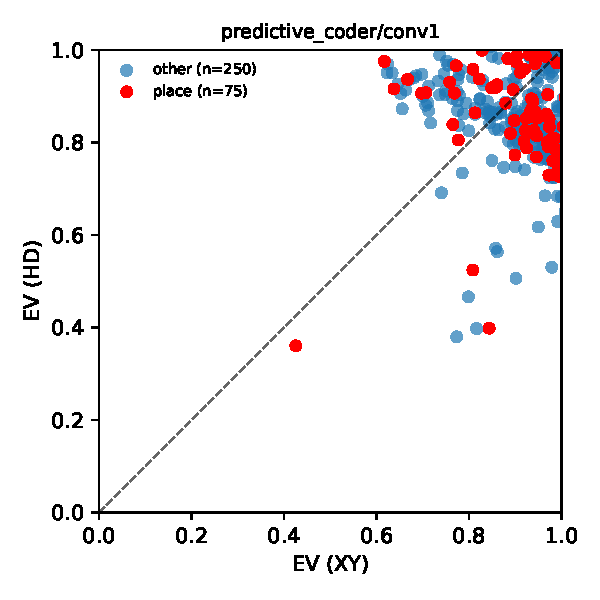
\includegraphics[width=0.23\textwidth]{figs/predictive_coder_conv1_ev_pitch.pdf}}
    \subfigure[down1]{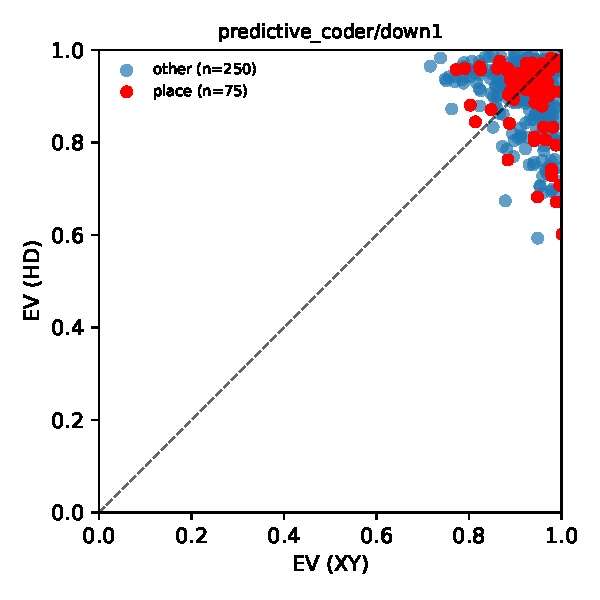
\includegraphics[width=0.23\textwidth]{figs/predictive_coder_down1_ev_pitch.pdf}}
    \subfigure[pre\_pred]{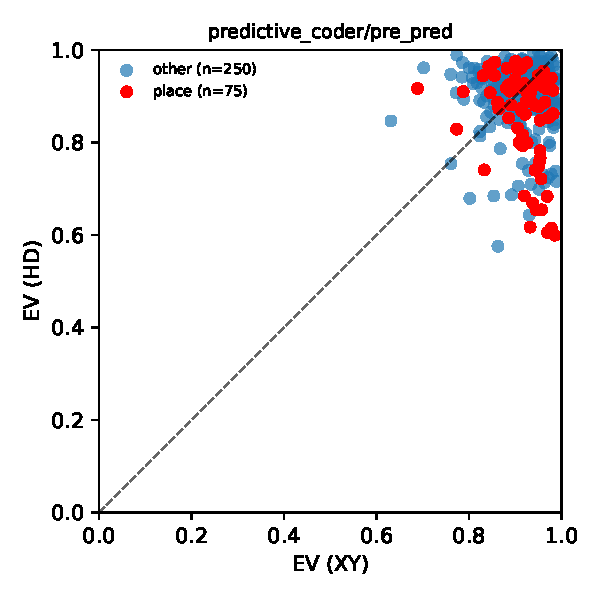
\includegraphics[width=0.23\textwidth]{figs/predictive_coder_pre_pred_ev_pitch.pdf}}
    \subfigure[post\_pred]{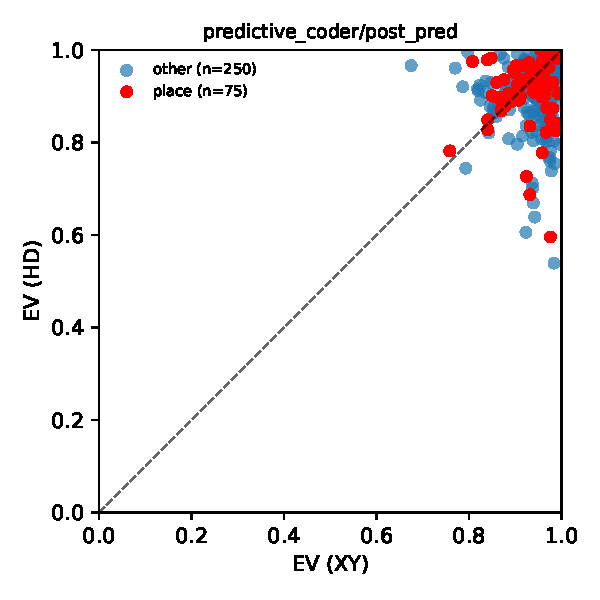
\includegraphics[width=0.23\textwidth]{figs/predictive_coder_post_pred_ev_pitch.pdf}}
    \caption{\textbf{Location and head direction explain comparable variance across all layers of the predictive-coding network.} Each panel shows the variance explained by 2-D location ($\mathrm{EV}_{xy}$, horizontal axis) versus by head direction ($\mathrm{EV}_{hd}$, vertical axis) for individual model units in one layer; the diagonal marks $\mathrm{EV}_{xy}=\mathrm{EV}_{hd}$. In every layer the population clusters near this diagonal, indicating that location and HD tuning are entangled throughout the network, consistent with the layers shown in Fig.~\ref{fig:pred} (bottom row).}
    \label{fig:si_pred_ev}
\end{figure}

\begin{figure}[h!]
    \centering
    \subfigure[VGG-16 \texttt{features.9}]{\includegraphics[width=0.36\textwidth]{{figs/vgg16_features.9_ev_pitch}.pdf}}
    \subfigure[untrained ResNet-50 \texttt{avgpool}]{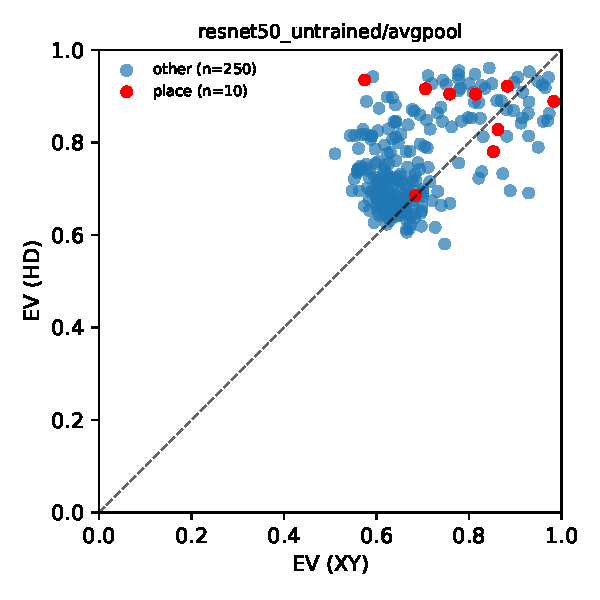
\includegraphics[width=0.36\textwidth]{figs/resnet50_untrained_avgpool_ev_pitch.pdf}}
    \caption{\textbf{Location and head direction explain comparable variance in other CNNs.} As in Fig.~\ref{fig:si_pred_ev}, for (a) an early layer of an ImageNet-pretrained VGG-16 and (b) the \texttt{avgpool} layer of a randomly initialized ResNet-50 (Fig.~\ref{fig:CNN} shows four layers of the pretrained ResNet-50). The trained VGG-16 layer lies on the $\mathrm{EV}_{xy}=\mathrm{EV}_{hd}$ diagonal like every trained layer we examined. The untrained network is the one exception: its units explain less variance overall and lean slightly towards head direction, and only 10 of its units pass the place-cell criteria.}
    \label{fig:si_cnn_ev}
\end{figure}

\subsection*{Scattered 3-D place$\times$HD firing fields in the CNN}

To visualize the tuning that underlies this entanglement, we plot the full 3-D ratemap over 2-D location and head direction for example CNN units that pass a standard 2-D place-cell classification. Unlike biological place cells, whose firing fields occupy the same location across head directions (Fig.~\ref{fig:PlaceCell}a,b), these units fire only for particular combinations of location and head direction, so their fields appear fragmented and scattered when the joint location$\times$HD volume is viewed slice-by-slice. This is the model-unit analogue of the joint-tuning breakdown shown for the predictive-coding network in Fig.~\ref{fig:pred}c.

\begin{figure}[h!]
    \centering
    \subfigure[]{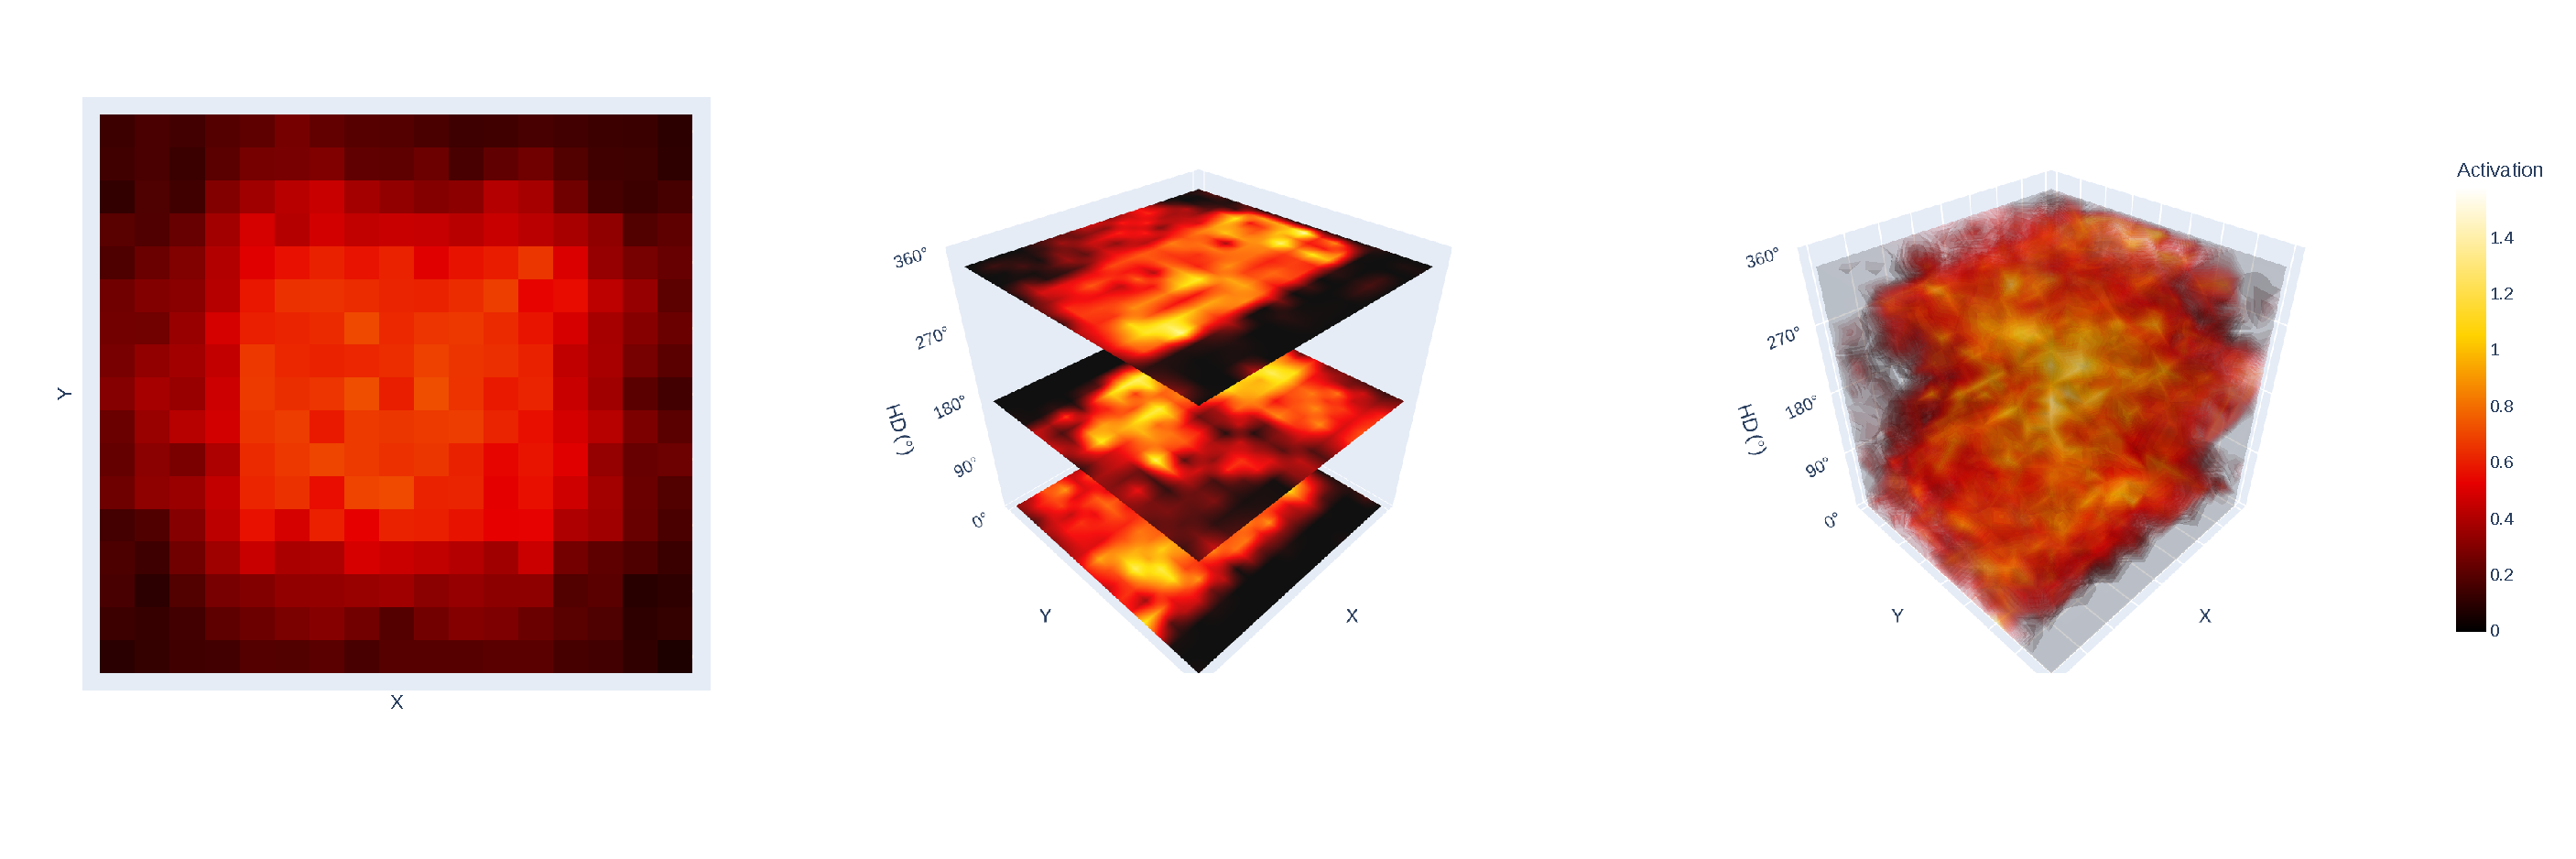
\includegraphics[width=0.85\textwidth]{figs/resnet50_layer3_N94.pdf}}\\
    \subfigure[]{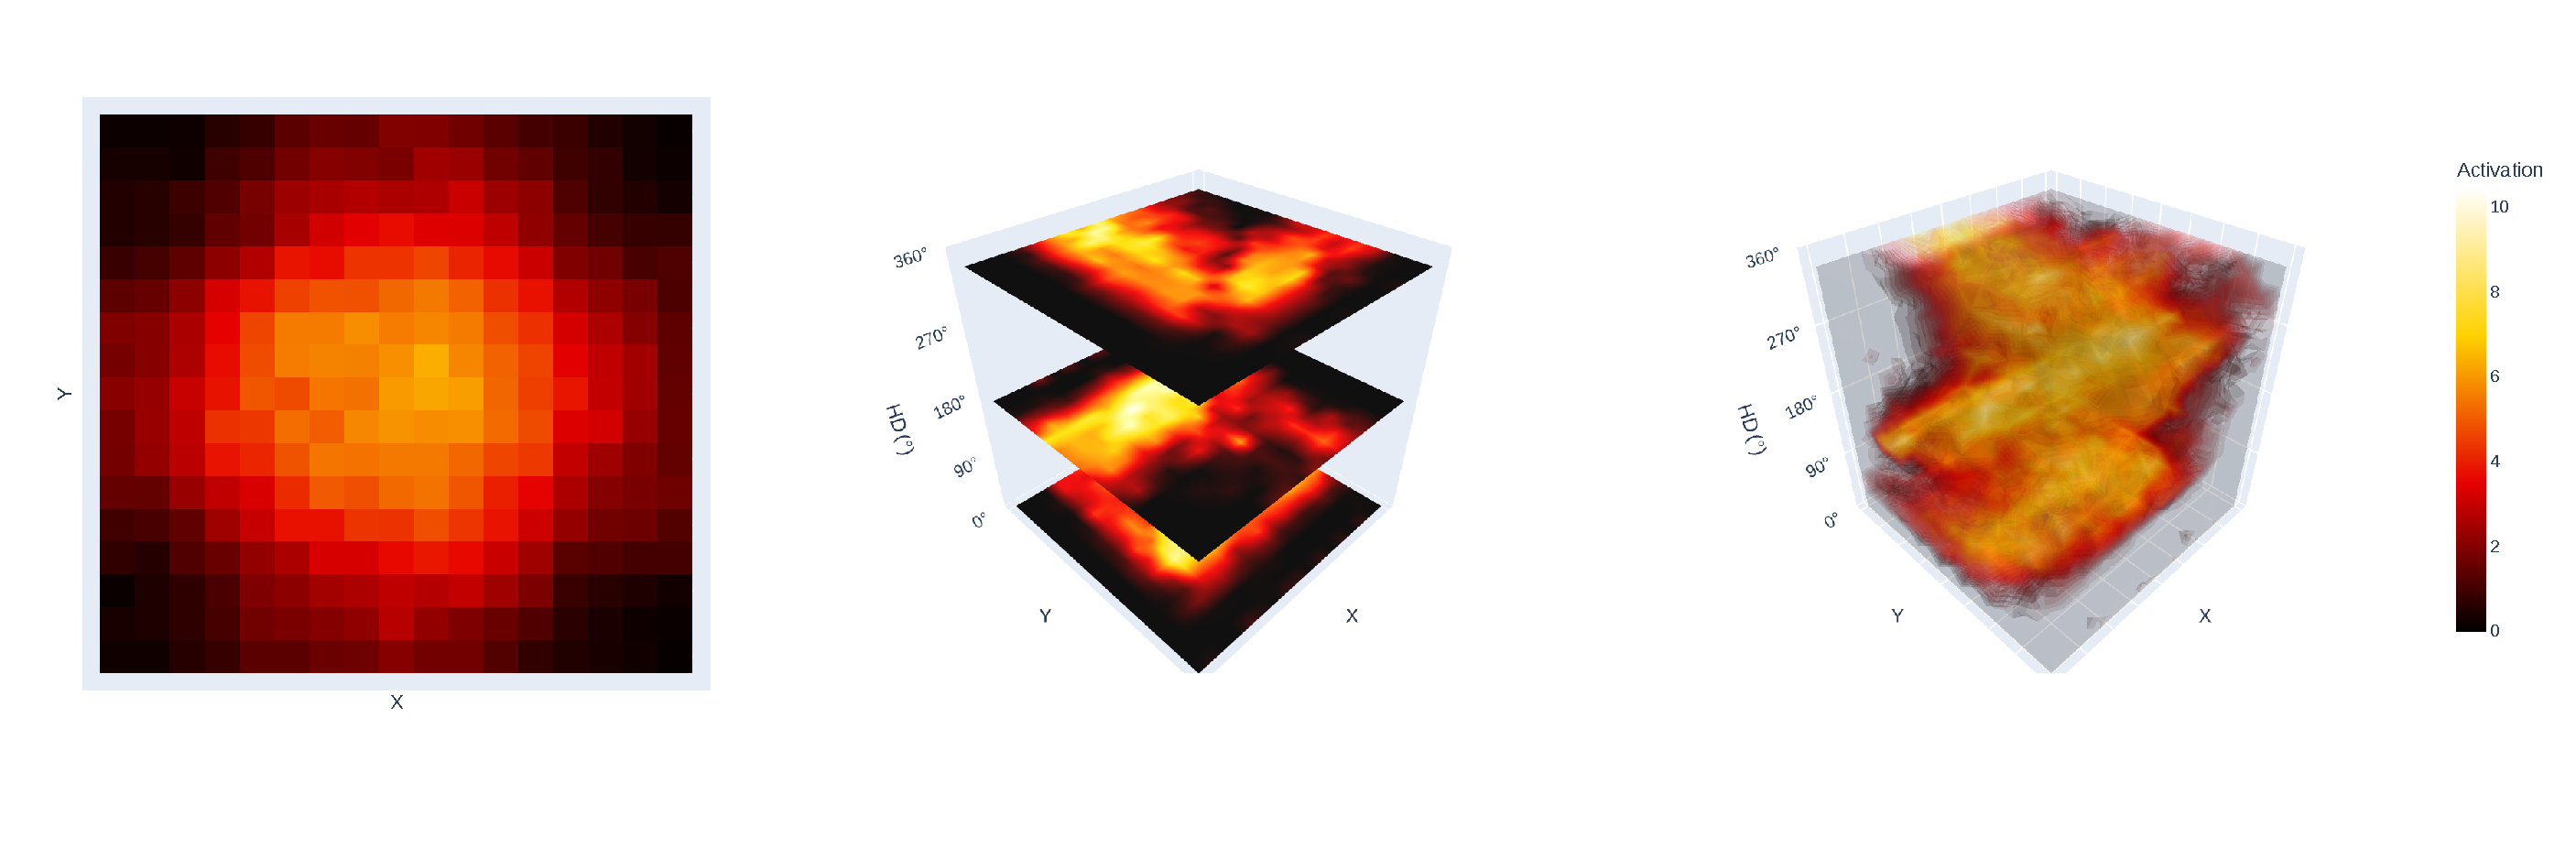
\includegraphics[width=0.85\textwidth]{figs/resnet50_layer3_N5619.pdf}}\\
    \subfigure[]{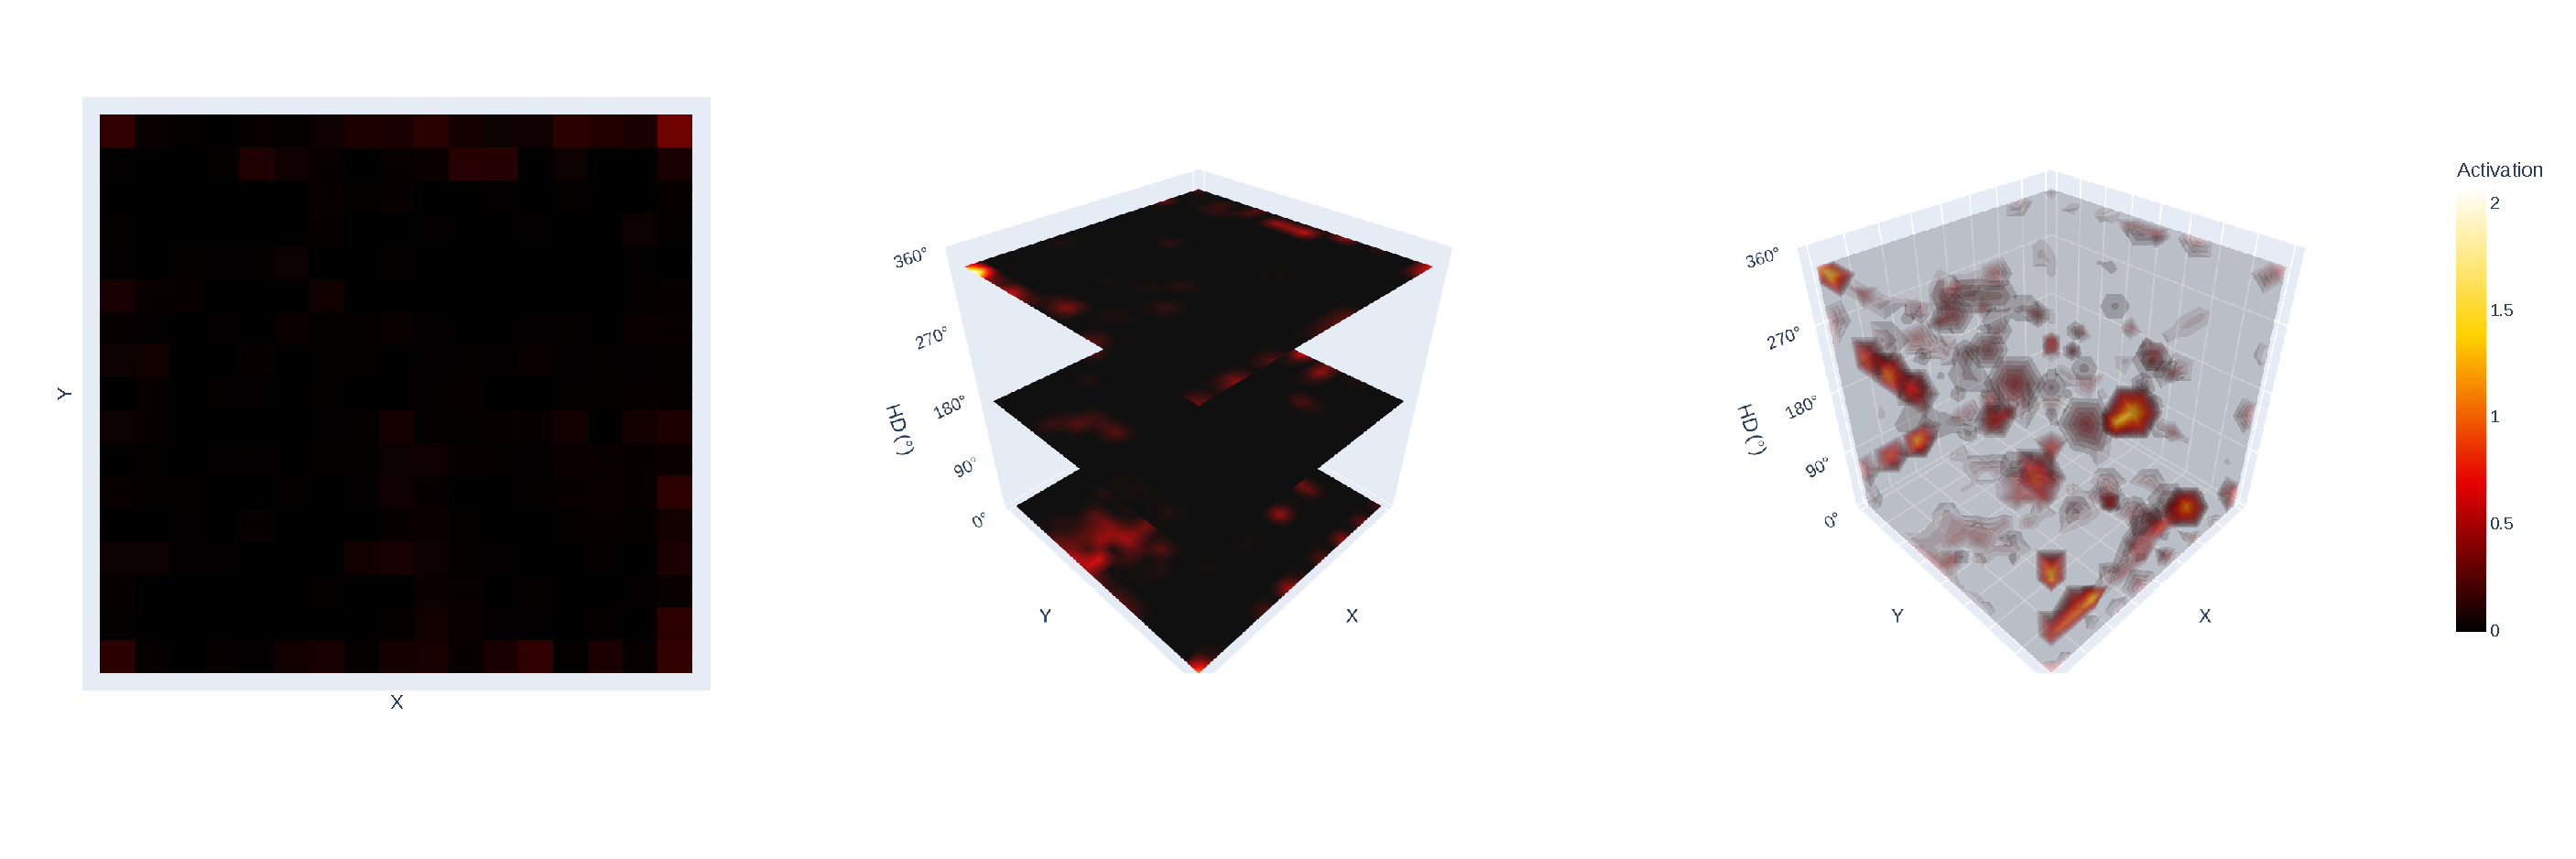
\includegraphics[width=0.85\textwidth]{figs/resnet50_layer4_N805.pdf}}
    \caption{\textbf{Firing fields of putative place-cell-like CNN units are scattered across the joint location--head-direction space.} Each panel shows the 3-D ratemap of one example ResNet-50 unit classified as a putative place cell, as a function of 2-D location and head direction (HD slices). High activity is confined to particular location--HD combinations rather than to a single HD-invariant location, so the place field breaks up across HD. This is the same phenomenon quantified by the near-diagonal variance partition in Figs.~\ref{fig:CNN} and \ref{fig:si_cnn_ev}.}
    \label{fig:si_scattered_maps}
\end{figure}

\subsection*{The finite-sampling floor of the split-half estimator}

A natural question is how the estimate depends on binning. With the cross-fold correlation estimator, binning itself introduces no bias: continuous and discretized (look-up-table) tuning functions give indistinguishable estimates. What binning does control is how many samples fall in each bin, and therefore the reliability $\langle C_{ii}\rangle_i$ of the two folds. On an axis the neuron is invariant to, the true $\mathrm{EV}$ is 0 but the estimate cannot fall below $1-\langle C_{ii}\rangle_i$, because even identical tuning curves estimated from two finite halves of the data correlate imperfectly. Fig.~\ref{fig:si_floor} shows this floor for the $\theta=0\degree$ simulation of Fig.~\ref{fig:estimation} as a function of the number of bins per axis and the number of samples. With $\gtrsim 4$ samples per bin the floor is a few hundredths and the raw $\mathrm{EV}(y)$ sits exactly on it; as the map becomes sparse (fewer than $\sim 1$ sample per bin, i.e., $\geq 30$ bins per axis at $N=1{,}000$, or $N\leq 500$ at $15\times15$ bins) the floor rises above 0.2 and a further positive bias appears that the normalization does not fully remove. The tuned axis is unaffected throughout ($\mathrm{EV}(x)\approx1$). In practice we therefore report raw $\mathrm{EV}$ together with the reliability, and treat values on an untuned axis that are comparable to $1-\langle C_{ii}\rangle_i$ as consistent with invariance (this is the situation for the place cells' $\mathrm{EV}_{hd}$ in Fig.~\ref{fig:PlaceCell}c, where the location$\times$HD map has $400\times60$ bins).

\begin{figure}[h!]
    \centering
    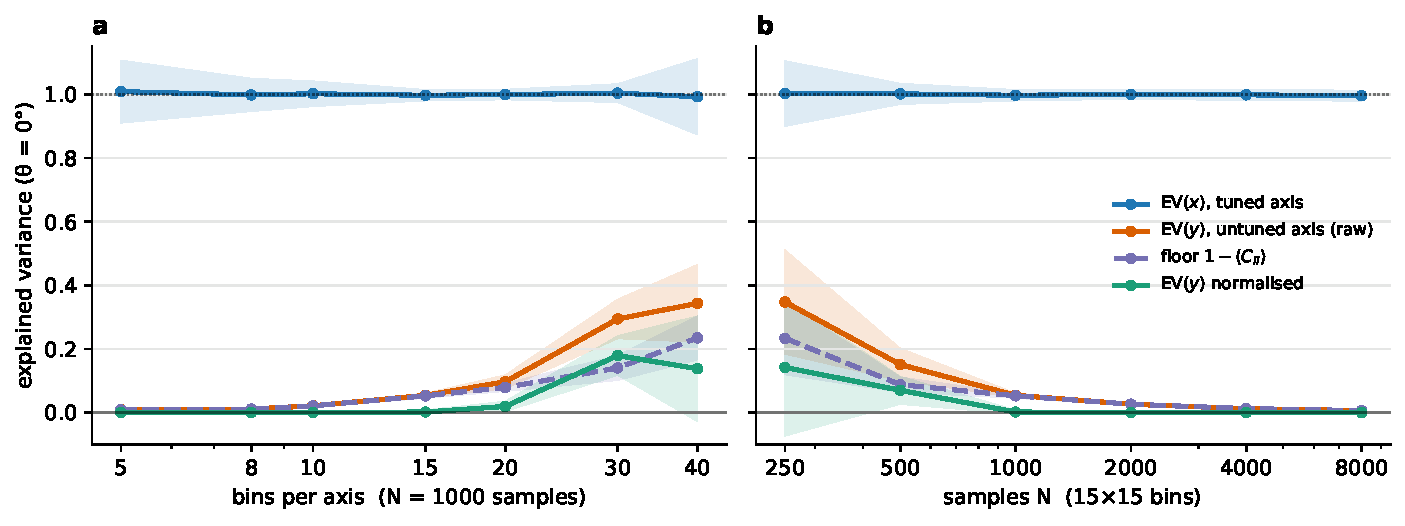
\includegraphics[width=0.95\textwidth]{figs/binning_noise_floor_sweep.pdf}
    \caption{\textbf{The split-half estimator's only bias is a finite-sampling floor set by the reliability of the two folds.} Simulated neuron tuned to $x$ only ($\theta=0\degree$), so the true $\mathrm{EV}(y)=0$ and $\mathrm{EV}(x)=1$. Lines are means and shaded bands $\pm1$~s.d. over 100 random split-half partitions. (a) Varying the number of bins per axis at $N=1{,}000$ samples. (b) Varying the number of samples at $15\times15$ bins. Blue: $\mathrm{EV}(x)$ on the tuned axis. Orange: raw $\mathrm{EV}(y)=1-\langle C_{ij}\rangle_{i\neq j}$ on the untuned axis. Dashed purple: the floor $1-\langle C_{ii}\rangle_i$. Green: reliability-normalized $\mathrm{EV}_{\mathrm{norm}}(y)$. The raw untuned-axis estimate tracks the floor until the map becomes sparse (fewer than about one sample per bin), where an additional bias appears; the tuned axis is recovered accurately in every condition.}
    \label{fig:si_floor}
\end{figure}


\end{document}